% Options for packages loaded elsewhere
\PassOptionsToPackage{unicode}{hyperref}
\PassOptionsToPackage{hyphens}{url}
%
\documentclass[
]{book}
\usepackage{amsmath,amssymb}
\usepackage{lmodern}
\usepackage{iftex}
\ifPDFTeX
  \usepackage[T1]{fontenc}
  \usepackage[utf8]{inputenc}
  \usepackage{textcomp} % provide euro and other symbols
\else % if luatex or xetex
  \usepackage{unicode-math}
  \defaultfontfeatures{Scale=MatchLowercase}
  \defaultfontfeatures[\rmfamily]{Ligatures=TeX,Scale=1}
\fi
% Use upquote if available, for straight quotes in verbatim environments
\IfFileExists{upquote.sty}{\usepackage{upquote}}{}
\IfFileExists{microtype.sty}{% use microtype if available
  \usepackage[]{microtype}
  \UseMicrotypeSet[protrusion]{basicmath} % disable protrusion for tt fonts
}{}
\makeatletter
\@ifundefined{KOMAClassName}{% if non-KOMA class
  \IfFileExists{parskip.sty}{%
    \usepackage{parskip}
  }{% else
    \setlength{\parindent}{0pt}
    \setlength{\parskip}{6pt plus 2pt minus 1pt}}
}{% if KOMA class
  \KOMAoptions{parskip=half}}
\makeatother
\usepackage{xcolor}
\usepackage{color}
\usepackage{fancyvrb}
\newcommand{\VerbBar}{|}
\newcommand{\VERB}{\Verb[commandchars=\\\{\}]}
\DefineVerbatimEnvironment{Highlighting}{Verbatim}{commandchars=\\\{\}}
% Add ',fontsize=\small' for more characters per line
\usepackage{framed}
\definecolor{shadecolor}{RGB}{248,248,248}
\newenvironment{Shaded}{\begin{snugshade}}{\end{snugshade}}
\newcommand{\AlertTok}[1]{\textcolor[rgb]{0.94,0.16,0.16}{#1}}
\newcommand{\AnnotationTok}[1]{\textcolor[rgb]{0.56,0.35,0.01}{\textbf{\textit{#1}}}}
\newcommand{\AttributeTok}[1]{\textcolor[rgb]{0.77,0.63,0.00}{#1}}
\newcommand{\BaseNTok}[1]{\textcolor[rgb]{0.00,0.00,0.81}{#1}}
\newcommand{\BuiltInTok}[1]{#1}
\newcommand{\CharTok}[1]{\textcolor[rgb]{0.31,0.60,0.02}{#1}}
\newcommand{\CommentTok}[1]{\textcolor[rgb]{0.56,0.35,0.01}{\textit{#1}}}
\newcommand{\CommentVarTok}[1]{\textcolor[rgb]{0.56,0.35,0.01}{\textbf{\textit{#1}}}}
\newcommand{\ConstantTok}[1]{\textcolor[rgb]{0.00,0.00,0.00}{#1}}
\newcommand{\ControlFlowTok}[1]{\textcolor[rgb]{0.13,0.29,0.53}{\textbf{#1}}}
\newcommand{\DataTypeTok}[1]{\textcolor[rgb]{0.13,0.29,0.53}{#1}}
\newcommand{\DecValTok}[1]{\textcolor[rgb]{0.00,0.00,0.81}{#1}}
\newcommand{\DocumentationTok}[1]{\textcolor[rgb]{0.56,0.35,0.01}{\textbf{\textit{#1}}}}
\newcommand{\ErrorTok}[1]{\textcolor[rgb]{0.64,0.00,0.00}{\textbf{#1}}}
\newcommand{\ExtensionTok}[1]{#1}
\newcommand{\FloatTok}[1]{\textcolor[rgb]{0.00,0.00,0.81}{#1}}
\newcommand{\FunctionTok}[1]{\textcolor[rgb]{0.00,0.00,0.00}{#1}}
\newcommand{\ImportTok}[1]{#1}
\newcommand{\InformationTok}[1]{\textcolor[rgb]{0.56,0.35,0.01}{\textbf{\textit{#1}}}}
\newcommand{\KeywordTok}[1]{\textcolor[rgb]{0.13,0.29,0.53}{\textbf{#1}}}
\newcommand{\NormalTok}[1]{#1}
\newcommand{\OperatorTok}[1]{\textcolor[rgb]{0.81,0.36,0.00}{\textbf{#1}}}
\newcommand{\OtherTok}[1]{\textcolor[rgb]{0.56,0.35,0.01}{#1}}
\newcommand{\PreprocessorTok}[1]{\textcolor[rgb]{0.56,0.35,0.01}{\textit{#1}}}
\newcommand{\RegionMarkerTok}[1]{#1}
\newcommand{\SpecialCharTok}[1]{\textcolor[rgb]{0.00,0.00,0.00}{#1}}
\newcommand{\SpecialStringTok}[1]{\textcolor[rgb]{0.31,0.60,0.02}{#1}}
\newcommand{\StringTok}[1]{\textcolor[rgb]{0.31,0.60,0.02}{#1}}
\newcommand{\VariableTok}[1]{\textcolor[rgb]{0.00,0.00,0.00}{#1}}
\newcommand{\VerbatimStringTok}[1]{\textcolor[rgb]{0.31,0.60,0.02}{#1}}
\newcommand{\WarningTok}[1]{\textcolor[rgb]{0.56,0.35,0.01}{\textbf{\textit{#1}}}}
\usepackage{longtable,booktabs,array}
\usepackage{calc} % for calculating minipage widths
% Correct order of tables after \paragraph or \subparagraph
\usepackage{etoolbox}
\makeatletter
\patchcmd\longtable{\par}{\if@noskipsec\mbox{}\fi\par}{}{}
\makeatother
% Allow footnotes in longtable head/foot
\IfFileExists{footnotehyper.sty}{\usepackage{footnotehyper}}{\usepackage{footnote}}
\makesavenoteenv{longtable}
\usepackage{graphicx}
\makeatletter
\def\maxwidth{\ifdim\Gin@nat@width>\linewidth\linewidth\else\Gin@nat@width\fi}
\def\maxheight{\ifdim\Gin@nat@height>\textheight\textheight\else\Gin@nat@height\fi}
\makeatother
% Scale images if necessary, so that they will not overflow the page
% margins by default, and it is still possible to overwrite the defaults
% using explicit options in \includegraphics[width, height, ...]{}
\setkeys{Gin}{width=\maxwidth,height=\maxheight,keepaspectratio}
% Set default figure placement to htbp
\makeatletter
\def\fps@figure{htbp}
\makeatother
\setlength{\emergencystretch}{3em} % prevent overfull lines
\providecommand{\tightlist}{%
  \setlength{\itemsep}{0pt}\setlength{\parskip}{0pt}}
\setcounter{secnumdepth}{5}
\usepackage{booktabs}
\usepackage{amsthm}
\makeatletter
\def\thm@space@setup{%
  \thm@preskip=8pt plus 2pt minus 4pt
  \thm@postskip=\thm@preskip
}
\makeatother
\ifLuaTeX
  \usepackage{selnolig}  % disable illegal ligatures
\fi
\IfFileExists{bookmark.sty}{\usepackage{bookmark}}{\usepackage{hyperref}}
\IfFileExists{xurl.sty}{\usepackage{xurl}}{} % add URL line breaks if available
\urlstyle{same} % disable monospaced font for URLs
\hypersetup{
  pdftitle={Analisis Resiko},
  pdfauthor={Bakti Siregar, M.Sc},
  hidelinks,
  pdfcreator={LaTeX via pandoc}}

\title{Analisis Resiko}
\author{Bakti Siregar, M.Sc}
\date{2023-05-22}

\begin{document}
\maketitle

{
\setcounter{tocdepth}{1}
\tableofcontents
}
\hypertarget{kata-pengantar}{%
\chapter*{Kata Pengantar}\label{kata-pengantar}}
\addcontentsline{toc}{chapter}{Kata Pengantar}

\hypertarget{deskripsi-buku}{%
\section*{Deskripsi Buku}\label{deskripsi-buku}}
\addcontentsline{toc}{section}{Deskripsi Buku}

\textbf{Analisa Resiko} adalah buku yang interaktif, online, dan tersedia secara gratis.

\begin{itemize}
\tightlist
\item
  Versi online berisi banyak objek interaktif (kuis, demonstrasi komputer, grafik interaktif, video, dan sejenisnya) yang dapat dipergunakan untuk menunjang \emph{pembelajaran lebih baik}.
\item
  Sebagian besar isi dari buku ini tersedia untuk \emph{dibaca offline} dalam format pdf dan EPUB.
\item
  Direncanakan akan tersedia dalam berbagai bahasa.
\end{itemize}

\hypertarget{petunjuk-penggunaan}{%
\subsection*{Petunjuk Penggunaan}\label{petunjuk-penggunaan}}
\addcontentsline{toc}{subsection}{Petunjuk Penggunaan}

Buku ini dapat dipergunakan dalam pembelajaran kurikulum aktuaria di seluruh dunia. Adapun cakupan pembelajarannya adalah analisa data kerugian dari berbagai organisasi aktuaria ternama didunia. Sehingga, buku ini cocok digunakan ditingkat universitas maupun pembelajar mandiri yang ingin lulus ujian aktuaria profesional. Selain itu, buku juga akan sangat berguna dalam pengembangan profesional berkelanjutan bagi para aktuaris maupun profesional lainnya di bidang asuransi dan industri terkait manajemen risiko keuangan.

\hypertarget{manfaat}{%
\subsection*{Manfaat}\label{manfaat}}
\addcontentsline{toc}{subsection}{Manfaat}

Salah satu manfaat penting dari buku online ini adalah pemerataan akses pengetahuan, sehingga memungkinkan masyarakat yang lebih luas untuk belajar tentang profesi aktuaria. Selain itu, setiap orang memiliki kapasitas untuk melibatkan banyak pihak melalui pembelajaran aktif yang memperdalam proses pembelajaran, menghasilkan analis terbaik dalam melakukan pekerjaan aktuaria yang solid.

Sekarang, pertanyaan besarnya adalah ``Mengapa buku ini baik untuk mahasiswa dan dosen serta orang lain yang terlibat dalam proses pembelajaran?'' Biaya adalah salah satu faktor yang sering disebut sebagai kendala utama bagi mahasiswa dan dosen dalam pemilihan buku teks. Selain itu, Mahasiswa sekarang ini lebih menyukai buku yang dapat dibawa secara secara elektronik (online).

\hypertarget{mengapa-analisa-resiko}{%
\subsection*{Mengapa Analisa Resiko?}\label{mengapa-analisa-resiko}}
\addcontentsline{toc}{subsection}{Mengapa Analisa Resiko?}

Tujuannya adalah agar buku ini pada akhirnya akan dapat dikembangkan secara serius kurikulum aktuaria. Mengingat perubahan era digital seperti sekarang ini akhirnya mendorong para aktuaris dalam melakukan analisa bergantung pada data yang dimiliki. Ide di balik nama \emph{Analisa Resiko} adalah untuk mengintegrasikan model data kerugian klasik dari probabilitas yang diterapkan dengan alat analitik modern. Secara khusus, penulis menyadari bahwa big data (termasuk media sosial dan asuransi berbasis penggunaan) akan terus berkembang dan komputasi berkecepatan tinggi sudah tersedia.

\hypertarget{ucapan-terima-kasih}{%
\section*{Ucapan Terima Kasih}\label{ucapan-terima-kasih}}
\addcontentsline{toc}{section}{Ucapan Terima Kasih}

Kami juga ingin mengucapkan terima kasih yang sebesar-sebesar pada semua pihak yang terlibat dalam pengembangan buku ini, yakni; mahasiswa-i, dosen, dan Universitas Matana atas dukungan dalam upaya bersama kami untuk menyediakan konten pendidikan dalam bidang aktuaria.


\includegraphics[width=0.5\textwidth,height=\textheight]{images/Logo.png}

\hypertarget{kontributor}{%
\section*{Kontributor}\label{kontributor}}
\addcontentsline{toc}{section}{Kontributor}

Sebagian besar dari isi buku ini diadopsi dari \textbf{\href{https://openacttexts.github.io/Loss-Data-Analytics/ChapIntro.html}{Loss Data Analytics}}. Berikut ini adalah nama-nama dan biografi singkat para penulis:

\begin{itemize}
\tightlist
\item
  \textbf{Bakti Siregar, M.Sc} adalah Kepala Program Studi dan Dosen di Jurusan Statistika Universitas Matana. Beliau juga seorang dosen yang juga bekerja sebagai ilmuwan data lepas yang memiliki antusiasme untuk analitik data besar, pembelajaran mesin, Pemodelan, dan pemecahan masalah. Orang menganggap saya programmer Matematika karena saya memiliki kemampuan yang kuat dalam program Statistik seperti R Studio, dan Python, dan juga akrab dengan alat basis data seperti MySQL dan sistem data besar baik Spark maupun Hadoop. Selain itu, saya dapat mengoperasikan salah satu perangkat lunak analitik bisnis yang paling kuat seperti Tableau.
\end{itemize}

\begin{itemize}
\tightlist
\item
  \textbf{Yosia} adalah salah satu mahasiwa terbaik di jurusan Statistika Universitas Matana. Dia juga memiliki minat dalam pembelajaran sains data dan akuturia khususnya melakukan komputasi dengan menggunakan R dan Python. Yosia bercita-cita suatu saat nanti akan menjadi seseorang yang ahli dibidang aktuaria maupun sain data. Yosia adalah mahasiswi jurusan Statistik di Universitas Matana. Dia memiliki minat teoretis yang luas serta minat dalam komputasi, ia juga sudah pernah terlibat dalam menerbitkan di jurnal Pengabdian Kepada Masyarakat \textbf{(PKM)}. Dia juga aktif dalam berbagai aktifitas organisasi kampus.
\end{itemize}

\begin{itemize}
\tightlist
\item
  \textbf{Clara Della} adalah mahasiswi jurusan Statistik di Universitas Matana. Dia memiliki minat teoretis yang luas serta minat dalam komputasi, ia juga sudah pernah terlibat dalam menerbitkan di jurnal Pengabdian Kepada Masyarakat \textbf{(PKM)}. Dia juga aktif dalam berbagai aktifitas organisasi kampus. adalah mahasiswi jurusan Statistik di Universitas Matana. Dia memiliki minat teoretis yang luas serta minat dalam komputasi, ia juga sudah pernah terlibat dalam menerbitkan di jurnal Pengabdian Kepada Masyarakat \textbf{(PKM)}. Dia juga aktif dalam berbagai aktifitas organisasi kampus.
\end{itemize}

\begin{itemize}
\tightlist
\item
  \textbf{Karen} adalah mahasiswi jurusan Statistik di Universitas Matana yang memiliki keahlian penelitiannya dengan menggunakan teori pemodelan, manajemen risiko, dan optimasi. adalah mahasiswi jurusan Statistik di Universitas Matana. Dia memiliki minat teoretis yang luas serta minat dalam komputasi, ia juga sudah pernah terlibat dalam menerbitkan di jurnal Pengabdian Kepada Masyarakat \textbf{(PKM)}. Dia juga aktif dalam berbagai aktifitas organisasi kampus.
\end{itemize}

\begin{itemize}
\tightlist
\item
  \textbf{Brigita} adalah dosen senior di Macquarie University di Australia, di mana ia menjabat sebagai direktur program sarjana aktuaria sejak 2018. Ia memperoleh gelar Ph.D.~pada tahun 2015 dari Nanyang Technological University di Singapura. Dia adalah seorang aktuaris yang berkualifikasi penuh, memegang kredensial dari US Society of Actuaries dan Australian Actuaries Institute. Minat penelitian utamanya adalah pemodelan kematian, manajemen risiko umur panjang, dan sistem bonus-malus.
\end{itemize}

\begin{itemize}
\tightlist
\item
  \textbf{Naufal} adalah seorang profesor di Universitas Matana. Dia memiliki gelar di bidang Matematika dan Ph.D.~dalam Sains: Matematika, diperoleh di University of Antwerp. Selama Ph.D., ia berhasil mengambil Magister Asuransi dan Magister Teknik Keuangan dan Aktuaria, keduanya di KU Leuven. Penelitiannya berfokus pada adaptasi dan penerapan metode statistik yang kuat untuk data asuransi dan keuangan. adalah mahasiswi jurusan Statistik di Universitas Matana. Dia memiliki minat teoretis yang luas serta minat dalam komputasi, ia juga sudah pernah terlibat dalam menerbitkan di jurnal Pengabdian Kepada Masyarakat \textbf{(PKM)}. Dia juga aktif dalam berbagai aktifitas organisasi kampus.
\end{itemize}

\begin{itemize}
\tightlist
\item
  \textbf{Garry} adalah Associate Professor di Departemen Manajemen Risiko, Asuransi, dan Kesehatan di Fox School of Business, Temple University? Dia adalah Associate dari Society of Actuaries. Dia mengajar mata kuliah Ilmu Aktuaria dan Manajemen Risiko di tingkat sarjana dan pascasarjana. Minat penelitiannya meliputi tata kelola perusahaan asuransi, manajemen modal, dan analisis sentimen. Dia menerima gelar Ph.D.~dari The Wharton School of the University of Pennsylvania.
\end{itemize}

\hypertarget{kritik-saran}{%
\section*{Kritik \& Saran}\label{kritik-saran}}
\addcontentsline{toc}{section}{Kritik \& Saran}

Buku teks interaktif yang tersedia secara gratis mewakili usaha baru dalam pendidikan aktuaria dan kami membutuhkan masukan Anda. Meskipun banyak upaya telah dilakukan untuk pengembangan, kami mengharapkan cegukan. Harap beri tahu instruktur Anda tentang peluang untuk peningkatan, hubungi kami melalui situs proyek kami, atau hubungi kontributor bab secara langsung dengan saran peningkatan.

Berikut ini dilampirkan beberapa peninjau atau pembaca yang telah memberikan saran dan pendapat mengenai pengembangan buku ini, adalah:

\begin{itemize}
\tightlist
\item
  mahasiswa 1
\item
  mahasiswa 2
\item
  mahasiswa 3
\item
  mahasiswa 4
\item
  mahasiswa 5
\item
  mahasiswa 6
\end{itemize}

<<<<<<< HEAD
\hypertarget{introduction-to-loss-data-analytics}{%
\chapter{Introduction to Loss Data Analytics}\label{introduction-to-loss-data-analytics}}

Chapter Preview. This book introduces readers to methods of analyzing insurance data. Section 1.1 begins with a discussion of why the use of data is important in the insurance industry. Section 1.2 gives a general overview of the purposes of analyzing insurance data which is reinforced in the Section 1.3 case study. Naturally, there is a huge gap between the broad goals summarized in the overview and a case study application; this gap is covered through the methods and techniques of data analysis covered in the rest of the text.
=======
\hypertarget{pengantar-analitika-data-kerugian}{%
\chapter{Pengantar Analitika Data Kerugian}\label{pengantar-analitika-data-kerugian}}

Preview Bab. Buku ini memperkenalkan pada metode analisis data asuransi. Bagian 1.1 dimulai dengan pembahasan mengapa penggunaan data itu penting dalam industri asuransi. Bagian 1.2 memberikan gambaran umum tentang tujuan analisis data asuransi yang diperkuat dalam studi kasus Bagian 1.3. Secara alami, ada kesenjangan besar antara tujuan umum yang dirangkum dalam gambaran dan aplikasi studi kasus. Kesenjangan ini dibahas melalui metode dan teknik analisis data yang tercakup dalam penjelasan berikutnya.

\hypertarget{relevansi-analitika-dalam-aktivitas-asuransi}{%
\section{Relevansi Analitika dalam Aktivitas Asuransi}\label{relevansi-analitika-dalam-aktivitas-asuransi}}

\begin{center}\rule{0.5\linewidth}{0.5pt}\end{center}

yang akan dipelajari dalam bab ini yaitu:

\begin{itemize}
\tightlist
\item
  Meringkas pentingnya asuransi bagi konsumen dan ekonomi
\item
  Menggambarkan analitika
\item
  Mengidentifikasi peristiwa penghasil data yang terkait dengan jangka waktu kontrak asuransi yang umum
\end{itemize}

\begin{center}\rule{0.5\linewidth}{0.5pt}\end{center}

\hypertarget{sifat-dan-relevansi-asuransi}{%
\subsection{Sifat dan Relevansi Asuransi}\label{sifat-dan-relevansi-asuransi}}

Buku ini memperkenalkan proses penggunaan data untuk mengambil keputusan dalam konteks asuransi. Buku ini tidak berasumsi bahwa pembaca sudah familiar dengan asuransi, tetapi memperkenalkan konsep-konsep asuransi sesuai kebutuhan. Jika baru mengenal asuransi, mungkin yang paling mudah adalah memikirkan sebuah polis asuransi yang mencakup isi apartemen atau rumah yang dapat di sewa (dikenal sebagai asuransi penyewa) atau isi dan properti dari bangunan yang dimiliki pribadi atau seorang teman (dikenal sebagai asuransi pemilik rumah). Contoh umum lainnya adalah asuransi mobil. Dalam kejadian kecelakaan, polis ini dapat mencakup kerusakan pada kendaraan pribadi, kerusakan pada kendaraan lain dalam kecelakaan tersebut, serta biaya medis bagi mereka yang terluka dalam kecelakaan.

Salah satu cara untuk memahami sifat asuransi adalah dengan melihat siapa yang membelinya. Asuransi penyewa, pemilik rumah, dan asuransi mobil adalah contoh asuransi personal, karena polis-polis ini diterbitkan untuk individu. Bisnis juga membeli asuransi, seperti perlindungan atas properti mereka, dan ini dikenal sebagai asuransi komersial. Penjualnya, perusahaan asuransi, juga dikenal sebagai penanggung. Bahkan perusahaan asuransi pun membutuhkan asuransi. Hal ini dikenal sebagai reasuransi.

Cara lain untuk memahami sifat asuransi adalah dengan jenis risiko yang dicakup. Di Amerika Serikat, kebijakan seperti asuransi penyewa dan pemilik rumah dikenal sebagai asuransi properti, sedangkan kebijakan seperti asuransi mobil yang mencakup kerusakan medis pada orang disebut asuransi kecelakaan. Di negara lain, keduanya dikenal sebagai asuransi non-hidup atau umum, untuk membedakannya dari asuransi jiwa.

Baik asuransi jiwa maupun asuransi non-hidup adalah komponen penting dalam ekonomi dunia. Institut Informasi Asuransi (2016) memperkirakan premi asuransi langsung di dunia untuk tahun 2014 sebesar 2.654.549 juta dolar AS untuk asuransi jiwa dan 2.123.699 juta dolar AS untuk asuransi non-hidup; angka-angka ini dalam jutaan dolar AS. Total tersebut mewakili 6,2\% dari produk domestik bruto (PDB) dunia. Dengan kata lain, asuransi jiwa menyumbang 55,5\% dari premi asuransi dan 3,4\% dari PDB dunia, sedangkan asuransi non-hidup menyumbang 44,5\% dari premi asuransi dan 2,8\% dari PDB dunia. Baik asuransi jiwa maupun asuransi non-hidup merupakan kegiatan ekonomi penting.

Asuransi mungkin tidak semenarik industri olahraga, tetapi asuransi memengaruhi kehidupan keuangan banyak orang. Dalam segala ukuran, asuransi merupakan kegiatan ekonomi yang besar. Seperti yang telah disebutkan sebelumnya, secara global, premi asuransi mencakup sekitar 6,2\% dari PDB dunia pada tahun 2014 (Institut Informasi Asuransi 2016). Sebagai contoh, premi asuransi menyumbang 18,9\% dari PDB di Taiwan (yang tertinggi dalam studi ini) dan mewakili 7,3\% dari PDB di Amerika Serikat. Pada tingkat pribadi, hampir setiap orang yang memiliki rumah memiliki asuransi untuk melindungi diri mereka dalam kejadian kebakaran, badai es, atau peristiwa bencana lainnya. Hampir setiap negara mengharuskan asuransi bagi mereka yang mengemudikan mobil. Secara keseluruhan, meskipun tidak terlalu menghibur, asuransi memainkan peran penting dalam perekonomian negara-negara dan kehidupan individu.

\hypertarget{apa-itu-analitika}{%
\subsection{Apa itu Analitika?}\label{apa-itu-analitika}}

Asuransi merupakan industri yang mengandalkan data. Seperti perusahaan-perusahaan besar dan organisasi lainnya, perusahaan asuransi menggunakan data ketika mencoba untuk menentukan berapa banyak yang harus dibayarkan kepada karyawan, berapa banyak karyawan yang harus dipertahankan, bagaimana cara memasarkan layanan dan produk mereka, bagaimana meramalkan tren keuangan, dan sebagainya. Hal ini mewakili bidang-bidang aktivitas umum yang tidak spesifik hanya untuk industri asuransi. Meskipun setiap industri memiliki nuansa dan kebutuhan data yang berbeda, pengumpulan, analisis, dan penggunaan data merupakan kegiatan yang dibagikan oleh semua, mulai dari raksasa internet hingga bisnis kecil, oleh organisasi publik dan pemerintah, dan tidak spesifik hanya untuk industri asuransi. Anda akan menemukan bahwa metode dan alat pengumpulan dan analisis data yang diperkenalkan dalam teks ini relevan untuk semua industri.

Dalam industri yang mengandalkan data, analitika merupakan kunci untuk mendapatkan dan mengekstraksi informasi dari data. Namun, apa itu analitika? Pengambilan keputusan bisnis yang didasarkan pada data telah dijelaskan sebagai analitika bisnis, inteligensi bisnis, dan ilmu data. Istilah-istilah ini, antara lain, kadang-kadang digunakan secara bergantian dan kadang-kadang mengacu pada aplikasi yang berbeda. Inteligensi bisnis mungkin fokus pada proses pengumpulan data, sering kali melalui basis data dan gudang data, sedangkan analitika bisnis menggunakan alat dan metode untuk analisis statistik data. Berbeda dengan dua istilah tersebut yang menekankan aplikasi bisnis, istilah ilmu data dapat mencakup aplikasi data yang lebih luas dalam berbagai domain ilmiah. Untuk tujuan kami, kami menggunakan istilah analitika untuk merujuk pada proses penggunaan data dalam pengambilan keputusan. Proses ini melibatkan pengumpulan data, pemahaman konsep dan model ketidakpastian, membuat inferensi umum, dan mengkomunikasikan hasil.

Ketika memperkenalkan metode data dalam teks ini, kami fokus pada kerugian yang timbul dari, atau terkait dengan, kewajiban dalam kontrak asuransi. Hal ini bisa berupa jumlah kerusakan pada apartemen seseorang dalam perjanjian asuransi penyewa, jumlah yang dibutuhkan untuk mengganti rugi seseorang yang Anda cedera dalam kecelakaan berkendara, dan sejenisnya. Kami menyebut jenis kewajiban ini sebagai klaim asuransi. Dengan fokus ini, kami dapat memperkenalkan dan langsung menggunakan alat dan teknik statistik yang umumnya berlaku.

\hypertarget{proses-asuransi}{%
\subsection{Proses Asuransi}\label{proses-asuransi}}

Cara lain untuk memahami sifat asuransi adalah melalui durasi kontrak asuransi, yang dikenal sebagai masa berlaku. Teks ini akan berfokus pada kontrak asuransi jangka pendek. Dalam konteks jangka pendek, kontrak asuransi umumnya memberikan perlindungan selama satu tahun atau enam bulan. Sebagian besar kontrak komersial dan personal berlaku selama satu tahun, sehingga itu adalah durasi default kami. Namun, terdapat pengecualian penting seperti kebijakan asuransi mobil di Amerika Serikat yang sering kali berlaku selama enam bulan.

Sebaliknya, biasanya kita menganggap asuransi jiwa sebagai kontrak jangka panjang di mana durasi default adalah beberapa tahun. Sebagai contoh, jika seseorang berusia 25 tahun membeli polis asuransi jiwa yang memberikan pembayaran saat meninggalnya tertanggung dan orang tersebut tidak meninggal sampai usia 100 tahun, maka kontrak tersebut berlaku selama 75 tahun.

Terdapat perbedaan penting lainnya antara produk asuransi jiwa dan non-jiwa. Dalam asuransi jiwa, jumlah manfaat sering ditetapkan dalam ketentuan kontrak. Sebaliknya, sebagian besar kontrak non-jiwa memberikan kompensasi atas kerugian tertanggung yang tidak diketahui sebelum terjadinya kecelakaan. (Biasanya terdapat batasan jumlah kompensasi yang ditetapkan.) Dalam kontrak asuransi jiwa yang berlaku selama bertahun-tahun, nilai waktu uang memainkan peran penting. Dalam kontrak non-jiwa, jumlah kompensasi yang acak menjadi prioritas.

Baik dalam asuransi jiwa maupun asuransi non-jiwa, frekuensi klaim sangat penting. Untuk banyak kontrak asuransi jiwa, peristiwa yang diasuransikan (seperti kematian) hanya terjadi sekali. Sebaliknya, dalam asuransi non-jiwa seperti asuransi mobil, umum bagi individu (terutama pengemudi pria muda) untuk mengalami lebih dari satu kecelakaan dalam setahun. Oleh karena itu, model-model kita perlu mencerminkan pengamatan ini; kami memperkenalkan berbagai model frekuensi yang juga mungkin Anda temui saat mempelajari asuransi jiwa.

Untuk asuransi jangka pendek, kerangka model probabilistiknya sederhana. Hanya mempertimbangkan model satu periode (panjang periode, misalnya satu tahun, akan ditentukan dalam situasi tersebut).

\begin{itemize}
\tightlist
\item
  Pada awal periode, tertanggung membayar premi yang diketahui kepada perusahaan asuransi sesuai kesepakatan antara kedua belah pihak dalam kontrak.
\item
  Pada akhir periode, perusahaan asuransi mengganti rugi tertanggung atas kerugian (mungkin multivariat) yang acak.
\end{itemize}

Kerangka kerja ini akan dikembangkan seiring berjalannya waktu, tetapi yang pertama fokus pada mengintegrasikan kerangka kerja ini dengan kekhawatiran tentang bagaimana data dapat muncul. Dari sudut pandang perusahaan asuransi, kontrak mungkin hanya berlaku selama satu tahun tetapi cenderung diperpanjang. Selain itu, pembayaran yang timbul dari klaim selama setahun dapat meluas jauh melebihi satu tahun. Salah satu cara untuk menggambarkan data yang muncul dari operasional perusahaan asuransi adalah dengan menggunakan pendekatan granular dengan garis waktu. Pendekatan proses memberikan gambaran keseluruhan tentang peristiwa yang terjadi selama masa berlaku kontrak asuransi, dan sifatnya - acak atau direncanakan, peristiwa kerugian (klaim) dan peristiwa perubahan kontrak, dan sebagainya. Dalam pandangan mikro ini, kita dapat memikirkan apa yang terjadi pada suatu kontrak pada berbagai tahap keberadaannya.

Gambar 1.1 menggambarkan garis waktu dari suatu kontrak asuransi yang khas. Sepanjang masa berlakunya kontrak, perusahaan secara rutin memproses peristiwa seperti pengumpulan premi dan penilaian, yang dijelaskan dalam Bagian 1.2; peristiwa-peristiwa ini ditandai dengan tanda \emph{x} pada garis waktu. Peristiwa-peristiwa yang tidak teratur dan tak terduga juga terjadi. Sebagai contoh, \(t_2\) dan \(t_4\) menandai peristiwa klaim asuransi (beberapa kontrak, seperti asuransi jiwa, mungkin hanya memiliki satu klaim). Waktu \(t_3\) dan \(t_5\) menandai peristiwa ketika pemegang polis ingin mengubah fitur-fitur tertentu dalam kontrak, seperti pilihan klaim dan jumlah perlindungan. Dari perspektif perusahaan, kita bahkan dapat mempertimbangkan inisiasi kontrak (kedatangan, waktu \(t_1\)) dan terminasi kontrak (kepergian, waktu \(t_6\)) sebagai peristiwa yang tidak pasti. (Sebagai alternatif, untuk beberapa tujuan, Anda dapat mengkondisikan peristiwa-peristiwa ini dan memperlakukannya sebagai pasti.)

( Gambar 1)

\hypertarget{operasi-perusahaan-asuransi}{%
\section{Operasi Perusahaan Asuransi}\label{operasi-perusahaan-asuransi}}

\begin{center}\rule{0.5\linewidth}{0.5pt}\end{center}

pada bab ini yang akan dipelajari adalah:

\begin{itemize}
\tightlist
\item
  Menggambarkan lima area operasional utama perusahaan asuransi.
\item
  Mengidentifikasi peran data dan peluang analitik dalam setiap area operasional.
\end{itemize}

\begin{center}\rule{0.5\linewidth}{0.5pt}\end{center}

Berdasarkan data asuransi, tujuan akhirnya adalah menggunakan data untuk mengambil keputusan. Kita akan mempelajari lebih lanjut tentang metode analisis dan ekstrapolasi data di bab-bab berikutnya. Untuk memulainya, mari kita pikirkan mengapa kita ingin melakukan analisis. Kita mengambil sudut pandang perusahaan asuransi (bukan orang yang diasuransikan) dan memperkenalkan cara untuk mendapatkan uang, membayarnya, mengelola biaya, dan memastikan bahwa kita memiliki cukup uang untuk memenuhi kewajiban. Penekanannya adalah pada operasi khusus asuransi daripada pada kegiatan bisnis umum seperti periklanan, pemasaran, dan manajemen sumber daya manusia.

Secara khusus, dalam banyak perusahaan asuransi, umumnya praktik untuk menggabungkan proses asuransi yang terperinci ke dalam unit operasional yang lebih besar; banyak perusahaan menggunakan area fungsional ini untuk memisahkan aktivitas karyawan dan tanggung jawab area tertentu. Aktuaris, analis keuangan lainnya, dan regulator asuransi bekerja dalam unit-unit ini dan menggunakan data untuk kegiatan-kegiatan berikut ini:

\emph{1. Memulai Asuransi}. Pada tahap ini, perusahaan membuat keputusan untuk menerima atau menolak risiko (tahap underwriting) dan menentukan premi yang sesuai (atau tarif). Analitik asuransi memiliki akar aktuaria dalam pembuatan tarif, di mana para analis berusaha untuk menentukan harga yang tepat untuk risiko yang tepat.

\emph{2. Memperbaharui Asuransi}. Banyak kontrak, terutama dalam asuransi umum, memiliki durasi yang relatif pendek seperti 6 bulan atau 1 tahun. Meskipun ada harapan implisit bahwa kontrak-kontrak tersebut akan diperbaharui, perusahaan asuransi memiliki kesempatan untuk menolak jaminan dan menyesuaikan premi. Analitik juga digunakan pada tahap perpanjangan polis ini di mana tujuannya adalah untuk mempertahankan pelanggan yang menguntungkan.

\emph{3. Manajemen Klaim}. Analitik telah lama digunakan dalam (1) mendeteksi dan mencegah penipuan klaim, (2) mengelola biaya klaim, termasuk mengidentifikasi dukungan yang tepat untuk biaya penanganan klaim, serta (3) memahami lapisan kelebihan untuk reasuransi dan retensi.

\emph{4. Reserving Kerugian}. Alat analitik digunakan untuk memberikan perkiraan yang tepat kepada manajemen mengenai kewajiban di masa depan dan untuk mengkuantifikasi ketidakpastian perkiraan tersebut.

\emph{5. Kesolvenan dan Alokasi Modal}. Menentukan jumlah modal yang diperlukan dan cara mengalokasikan modal di antara investasi-alternatif juga merupakan kegiatan analitik penting. Perusahaan harus memahami berapa banyak modal yang dibutuhkan agar mereka memiliki aliran kas yang cukup tersedia untuk memenuhi kewajiban mereka pada saat yang diharapkan (kesolvenan). Ini adalah pertanyaan penting yang tidak hanya menyangkut manajer perusahaan tetapi juga pelanggan, pemegang saham perusahaan, otoritas pengawas, serta masyarakat secara umum. Terkait dengan isu berapa banyak modal adalah pertanyaan tentang bagaimana mengalokasikan modal ke proyek keuangan yang berbeda, biasanya untuk memaksimalkan pengembalian investor. Meskipun pertanyaan ini dapat muncul pada beberapa tingkat, perusahaan asuransi umumnya tertarik dengan cara mengalokasikan modal ke berbagai lini bisnis dalam perusahaan dan ke anak perusahaan dari perusahaan induk.

Meskipun data merupakan komponen penting dari kesolvenan dan alokasi modal, komponen lain termasuk kerangka ekonomi lokal dan global, lingkungan investasi keuangan, dan persyaratan yang sangat spesifik sesuai dengan lingkungan regulasi saat ini, juga penting. Karena latar belakang yang diperlukan untuk mengatasi komponen-komponen ini, kami tidak membahas isu-isu kesolvenan, alokasi modal, dan regulasi dalam teks ini.

Namun demikian, untuk semua fungsi operasional, kami menekankan bahwa analitik dalam industri asuransi bukanlah latihan yang dapat dilakukan oleh sekelompok kecil analis sendiri. Hal ini membutuhkan perusahaan asuransi untuk melakukan investasi yang signifikan dalam teknologi informasi, pemasaran, underwriting, dan aktuaria. Karena area-area ini merupakan tujuan akhir utama dari analisis data, penjelasan tambahan tentang masing-masing unit operasional diberikan dalam subseksi berikutnya.

\hypertarget{memulai-asuransi}{%
\subsection{Memulai Asuransi}\label{memulai-asuransi}}

Menentukan harga produk asuransi bisa menjadi masalah yang membingungkan. Hal ini berbeda dengan industri lain seperti manufaktur di mana biaya suatu produk (relatif) diketahui dan menjadi acuan untuk menilai harga permintaan pasar. Demikian pula, dalam bidang layanan keuangan lainnya, harga pasar tersedia dan menjadi dasar untuk struktur penetapan harga yang sesuai dengan pasar produk. Namun, untuk banyak jenis asuransi, biaya suatu produk tidak pasti dan harga pasar tidak tersedia. Harapan atas biaya acak adalah tempat yang wajar untuk memulai penetapan harga. (Jika Anda telah mempelajari keuangan, maka Anda akan mengingat bahwa harapan adalah harga optimal untuk perusahaan asuransi yang netral terhadap risiko.) Dalam penetapan harga asuransi, sudah menjadi tradisi untuk memulai dengan biaya yang diharapkan. Perusahaan asuransi kemudian menambahkan margin untuk memperhitungkan tingkat risiko produk, biaya yang dikeluarkan dalam pelayanan produk, dan alokasi keuntungan/surplus perusahaan.

Penggunaan biaya yang diharapkan sebagai dasar penetapan harga umum terjadi dalam beberapa jenis bisnis asuransi. Ini termasuk asuransi mobil dan asuransi pemilik rumah. Dalam jenis asuransi ini, analitik telah membantu meningkatkan ketepatan perhitungan biaya yang diharapkan dari produk. Ketersediaan internet yang semakin luas bagi konsumen juga mendorong transparansi dalam penetapan harga; di pasar saat ini, konsumen memiliki akses mudah ke kutipan kompetitif dari sejumlah perusahaan asuransi. Perusahaan asuransi berusaha meningkatkan pangsa pasarnya dengan menyempurnakan sistem klasifikasi risiko mereka, sehingga mencapai perkiraan yang lebih baik mengenai harga produk dan memungkinkan strategi underwriting yang selektif (``cream-skimming'' adalah istilah yang digunakan ketika perusahaan asuransi hanya mengasuransikan risiko terbaik). Survei (misalnya, Earnix (2013)) menunjukkan bahwa penetapan harga adalah penggunaan analitik yang paling umum di kalangan perusahaan asuransi.

Underwriting, yaitu proses mengklasifikasikan risiko ke dalam kategori homogen dan mengalokasikan pemegang polis ke dalam kategori-kategori tersebut, merupakan inti dari penetapan tarif. Pemegang polis dalam satu kelas (kategori) memiliki profil risiko yang serupa sehingga dikenakan tarif asuransi yang sama. Ini adalah konsep premi yang adil secara aktuaria; adil untuk mengenakan tarif yang berbeda kepada pemegang polis hanya jika mereka dapat dibedakan berdasarkan faktor risiko yang dapat diidentifikasi. Sebuah artikel awal, Two Studies in Automobile Insurance Ratemaking (Bailey dan LeRoy 1960), memberikan dorongan bagi penerimaan metode analitik dalam industri asuransi. Makalah ini membahas masalah klasifikasi penetapan tarif asuransi mobil. Artikel tersebut menggambarkan contoh asuransi mobil yang memiliki lima kelas penggunaan yang saling berkaitan dengan empat kelas rating prestasi. Pada saat itu, kontribusi premi untuk kelas penggunaan dan rating prestasi ditentukan secara independen satu sama lain. Memikirkan efek interaksi dari variabel klasifikasi yang berbeda merupakan masalah yang lebih rumit.

Saat risiko pertama kali diperoleh, kewajiban perusahaan asuransi dapat dikelola dengan menerapkan parameter kontrak yang mengubah pembayaran kontrak. Bab 3 menjelaskan modifikasi umum termasuk co-insurance, deduktibel, dan batas atas kebijakan.

\hypertarget{memperbarui-asuransi}{%
\subsection{Memperbarui Asuransi}\label{memperbarui-asuransi}}

Asuransi merupakan jenis layanan keuangan dan, seperti banyak kontrak layanan lainnya, cakupan asuransi sering kali disepakati untuk jangka waktu terbatas di mana komitmen cakupan diselesaikan. Terutama untuk asuransi umum, kebutuhan akan cakupan terus berlanjut, dan oleh karena itu upaya dilakukan untuk mengeluarkan kontrak baru yang memberikan cakupan serupa ketika kontrak yang ada mencapai akhir masa berlakunya. Ini disebut perpanjangan polis. Isu perpanjangan juga dapat muncul dalam asuransi jiwa, misalnya, asuransi jiwa berjangka (sementara). Pada saat yang sama, kontrak lain seperti pensiun dini berakhir pada saat kematian tertanggung, sehingga masalah perpanjangan tidak relevan.

Dalam ketiadaan pembatasan hukum, saat perpanjangan polis, perusahaan asuransi memiliki kesempatan untuk:

\begin{itemize}
\tightlist
\item
  menerima atau menolak menerbitkan risiko tersebut; dan
\item
  menentukan premi baru, mungkin dengan melakukan klasifikasi ulang terhadap risiko tersebut.
\end{itemize}

Klasifikasi risiko dan penilaian saat perpanjangan didasarkan pada dua jenis informasi. Pertama, pada tahap awal, perusahaan asuransi memiliki banyak variabel penilaian yang dapat digunakan untuk pengambilan keputusan. Banyak variabel yang kemungkinan tidak akan berubah, misalnya jenis kelamin, sedangkan yang lain kemungkinan akan berubah, misalnya usia, dan yang lainnya mungkin berubah atau tidak, misalnya skor kredit. Kedua, berbeda dengan tahap awal, saat perpanjangan, perusahaan asuransi memiliki riwayat pengalaman kerugian dari pemegang polis, dan riwayat ini dapat memberikan wawasan tentang pemegang polis yang tidak tersedia dari variabel penilaian. Modifikasi premi berdasarkan riwayat klaim dikenal sebagai penilaian berdasarkan pengalaman, juga kadang-kadang disebut sebagai penilaian berdasarkan prestasi.

Metode penilaian berdasarkan pengalaman dapat diterapkan secara retrospektif atau prospektif. Dengan metode retrospektif, sebagian premi dikembalikan kepada pemegang polis dalam kejadian pengalaman yang menguntungkan bagi perusahaan asuransi. Premi retrospektif umum dalam perjanjian asuransi jiwa (di mana pemegang polis memperoleh dividen di Amerika Serikat, bonus di Inggris, dan pembagian keuntungan dalam cakupan asuransi jiwa sementara di Israel). Pada umumnya, metode prospektif lebih umum digunakan dalam asuransi umum, di mana pengalaman yang menguntungkan bagi pemegang polis akan dihargai melalui premi perpanjangan yang lebih rendah.

Riwayat klaim dapat memberikan informasi tentang minat risiko pemegang polis. Sebagai contoh, dalam asuransi personal, umumnya digunakan variabel untuk menunjukkan apakah klaim telah terjadi dalam tiga tahun terakhir atau tidak. Sebagai contoh lain, dalam asuransi komersial seperti asuransi kecelakaan kerja, dapat dilihat frekuensi atau tingkat keparahan klaim rata-rata pemegang polis selama tiga tahun terakhir. Riwayat klaim dapat mengungkapkan informasi yang sebaliknya tersembunyi (bagi perusahaan asuransi) tentang pemegang polis.

\hypertarget{pengelolaan-klaim-dan-produk}{%
\subsection{Pengelolaan Klaim dan Produk}\label{pengelolaan-klaim-dan-produk}}

Dalam beberapa jenis asuransi, proses pembayaran klaim untuk peristiwa yang diasuransikan relatif sederhana. Misalnya, dalam asuransi jiwa, sertifikat kematian sederhana sudah cukup untuk membayarkan jumlah manfaat sesuai dengan kontrak. Namun, dalam bidang asuransi properti dan kecelakaan, prosesnya bisa jauh lebih kompleks. Bayangkan peristiwa yang diasuransikan yang relatif sederhana seperti kecelakaan mobil. Di sini, seringkali diperlukan untuk menentukan pihak yang bertanggung jawab dan kemudian perlu mengevaluasi kerusakan pada semua kendaraan dan orang yang terlibat dalam insiden, baik yang diasuransikan maupun yang tidak diasuransikan. Selain itu, biaya yang dikeluarkan dalam mengevaluasi kerusakan juga harus dinilai, dan sebagainya. Proses menentukan cakupan, tanggung jawab hukum, dan penyelesaian klaim dikenal sebagai penyesuaian klaim.

Manajer asuransi terkadang menggunakan istilah ``kebocoran klaim'' untuk merujuk pada dolar yang hilang melalui ketidakefisienan pengelolaan klaim. Ada banyak cara di mana analitik dapat membantu mengelola proses klaim, lihat Gorman dan Swenson (2013). Secara historis, yang paling penting adalah pendeteksian penipuan. Proses penyesuaian klaim melibatkan mengurangi asimetri informasi (klaiman mengetahui apa yang terjadi; perusahaan mengetahui sebagian dari apa yang terjadi). Mengurangi penipuan adalah bagian penting dari proses pengelolaan klaim.

Deteksi penipuan hanyalah satu aspek dari pengelolaan klaim. Lebih luas lagi, kita dapat mempertimbangkan pengelolaan klaim terdiri dari komponen-komponen berikut:

\emph{- Pemilahan klaim.} Seperti dalam dunia medis, identifikasi dini dan penanganan yang tepat terhadap klaim dengan biaya tinggi (pasien, dalam dunia medis) dapat menghasilkan penghematan yang dramatis. Misalnya, dalam asuransi kecelakaan kerja, perusahaan asuransi berupaya untuk mengidentifikasi secara dini klaim-klaim yang berisiko mengakibatkan biaya medis tinggi dan periode pembayaran yang lama. Intervensi dini dalam kasus-kasus ini dapat memberikan perusahaan asuransi lebih banyak kendali atas penanganan klaim, perawatan medis, dan biaya secara keseluruhan dengan kembalinya pekerja lebih awal.

\emph{- Pengolahan klaim.} Tujuannya adalah menggunakan analitik untuk mengidentifikasi situasi rutin yang diperkirakan memiliki pembayaran kecil. Situasi yang lebih kompleks mungkin memerlukan penyesuaian oleh penyelesaian klaim yang berpengalaman dan bantuan hukum untuk menangani klaim dengan potensi pembayaran besar.

\emph{- Keputusan penyesuaian.} Setelah klaim kompleks diidentifikasi dan ditugaskan kepada penyelesaian klaim, rutinitas yang didorong oleh analitik dapat dibentuk untuk membantu proses pengambilan keputusan berikutnya. Proses tersebut juga dapat membantu penyelesaian klaim dalam mengembangkan cadangan kasus, perkiraan kewajiban finansial perusahaan asuransi di masa depan. Ini adalah masukan penting untuk cadangan kerugian perusahaan asuransi, yang dijelaskan dalam Bagian 1.2.4.

Selain penggantian kerugian kepada tertanggung, perusahaan asuransi juga perlu memperhatikan sumber lain yang mengalirkan pendapatan, yaitu biaya. Biaya penyesuaian kerugian merupakan bagian dari biaya pengelolaan klaim oleh perusahaan asuransi. Analitik dapat digunakan untuk mengurangi biaya yang terkait langsung dengan penanganan klaim (dialokasikan) serta waktu staf umum untuk mengawasi proses klaim (tidak dialokasikan). Industri asuransi memiliki biaya operasional yang tinggi dibandingkan dengan sektor jasa keuangan lainnya.

Selain pembayaran klaim, terdapat banyak cara lain di mana perusahaan asuransi menggunakan data untuk mengelola produk mereka. Kami telah membahas kebutuhan analitik dalam penjaminan, yaitu klasifikasi risiko pada tahap akuisisi awal dan tahap perpanjangan. Perusahaan asuransi juga tertarik untuk mengetahui pemegang polis mana yang memilih untuk memperpanjang kontrak mereka dan, seperti halnya dengan produk lainnya, memantau loyalitas pelanggan.

Analitik juga dapat digunakan untuk mengelola portofolio atau kumpulan risiko yang telah diperoleh oleh perusahaan asuransi. Seperti yang dijelaskan dalam Bab 10, setelah kontrak disepakati dengan tertanggung, perusahaan asuransi masih dapat mengubah kewajibannya bersih dengan melakukan perjanjian reasuransi. Jenis perjanjian ini melibatkan perusahaan reasuransi, yaitu perusahaan asuransi bagi perusahaan asuransi lainnya. Umum bagi perusahaan asuransi untuk membeli asuransi atas portofolio risiko mereka guna mendapatkan perlindungan dari peristiwa yang tidak biasa, sama seperti individu dan perusahaan lainnya.

\hypertarget{penyisihan-klaim}{%
\subsection{Penyisihan Klaim}\label{penyisihan-klaim}}

Fitur penting yang membedakan asuransi dari sektor lain dalam ekonomi adalah waktu pertukaran pertimbangan. Dalam industri manufaktur, pembayaran untuk barang umumnya dilakukan pada saat transaksi. Sebaliknya, dalam asuransi, uang yang diterima dari pelanggan terjadi sebelum manfaat atau layanan diberikan; ini diberikan pada tanggal yang lebih kemudian jika terjadi peristiwa tertanggung. Hal ini mengakibatkan kebutuhan untuk memiliki cadangan kekayaan guna memenuhi kewajiban di masa depan sehubungan dengan kewajiban yang dibuat, dan untuk memperoleh kepercayaan dari tertanggung bahwa perusahaan akan mampu memenuhi komitmennya. Besarannya cadangan kekayaan ini, dan pentingnya memastikan kecukupannya, merupakan perhatian utama bagi industri asuransi.

Mengalokasikan uang untuk klaim yang belum dibayar dikenal sebagai penyisihan kerugian; di beberapa yurisdiksi, cadangan ini juga dikenal sebagai ketentuan teknis. Seperti yang terlihat pada Gambar 1.1 beberapa kali di mana perusahaan merangkum posisi keuangannya; waktu-waktu ini dikenal sebagai tanggal penilaian. Klaim yang muncul sebelum tanggal penilaian telah dibayarkan, sedang dalam proses pembayaran, atau akan segera dibayarkan; klaim di masa depan setelah tanggal penilaian ini tidak diketahui. Perusahaan harus memperkirakan kewajiban yang belum diselesaikan ini ketika menentukan kekuatan keuangannya. Menentukan dengan tepat penyisihan kerugian penting bagi perusahaan asuransi atas banyak alasan.

\begin{enumerate}
\def\labelenumi{\arabic{enumi}.}
\item
  Penyisihan kerugian merupakan klaim yang diantisipasi yang perusahaan asuransi harus bayarkan kepada pelanggannya. Ketidakcukupan penyisihan dapat mengakibatkan ketidakmampuan untuk memenuhi kewajiban klaim. Sebaliknya, perusahaan asuransi dengan penyisihan berlebihan dapat menunjukkan perkiraan kelebihan cadangan yang konservatif dan dengan demikian menggambarkan posisi keuangan yang lebih lemah daripada yang sebenarnya.
\item
  Penyisihan memberikan perkiraan untuk biaya asuransi yang belum dibayar yang dapat digunakan untuk penetapan harga kontrak.
\item
  Penyisihan kerugian ini diperlukan oleh hukum dan peraturan. Masyarakat memiliki kepentingan yang kuat terhadap kekuatan keuangan dan solvabilitas perusahaan asuransi.
\item
  Selain regulator, pemangku kepentingan lain seperti manajemen perusahaan asuransi, investor, dan pelanggan membuat keputusan yang bergantung pada penyisihan kerugian perusahaan. Sementara regulator dan pelanggan menghargai perkiraan yang konservatif terkait klaim yang belum dibayar, manajer dan investor mencari perkiraan yang lebih objektif untuk mewakili kesehatan keuangan yang sebenarnya dari perusahaan.
\end{enumerate}

Penyisihan kerugian adalah topik di mana terdapat perbedaan yang signifikan antara asuransi jiwa dan asuransi umum (juga dikenal sebagai asuransi harta benda dan kecelakaan, atau asuransi non-jiwa). Dalam asuransi jiwa, tingkat keparahan (besaran kerugian) seringkali bukan sumber ketidakpastian karena pembayaran telah ditentukan dalam kontrak. Tingkat kejadian, yang dipengaruhi oleh kematian tertanggung, menjadi perhatian. Namun, karena waktu yang lama untuk penyelesaian kontrak asuransi jiwa, ketidakpastian nilai waktu uang yang diukur dari penerbitan hingga tanggal pembayaran dapat mendominasi perhatian tingkat kejadian. Sebagai contoh, bagi seorang tertanggung yang membeli kontrak asuransi jiwa pada usia 20 tahun, tidak jarang kontrak masih berlaku setelah 60 tahun, ketika tertanggung merayakan ulang tahun ke-80. Lihat, misalnya, Bowers et al.~(1986) atau Dickson, Hardy, dan Waters (2013) untuk pengenalan terhadap penyisihan kerugian dalam asuransi jiwa. Sebaliknya, untuk sebagian besar jenis bisnis asuransi non-jiwa, tingkat keparahan adalah sumber ketidakpastian utama dan durasi kontrak cenderung lebih singkat.
>>>>>>> 8262f607f9dc7e5f0fc37260e399a3d9592a7925

\hypertarget{frequency-modeling}{%
\chapter{Frequency Modeling}\label{frequency-modeling}}

\hypertarget{goodness-of-fit}{%
\section{Goodness of Fit}\label{goodness-of-fit}}

\hypertarget{modeling-loss-severity}{%
\chapter{Modeling Loss Severity}\label{modeling-loss-severity}}

<<<<<<< HEAD
=======
<<<<<<< HEAD
=======
<<<<<<< HEAD
=======
\hypertarget{basic-distributional-quantities}{%
\section{Basic Distributional Quantities}\label{basic-distributional-quantities}}

>>>>>>> 8262f607f9dc7e5f0fc37260e399a3d9592a7925
>>>>>>> 1507448987ea466b9753eba8674625da5f907a7f
>>>>>>> f9a746c5b24126443ff5b71c4335db228507f5bc
\hypertarget{modifikasi-pertanggungan}{%
\section{modifikasi pertanggungan}\label{modifikasi-pertanggungan}}

Coverage modifications atau modifikasi pertanggungan adalah perubahan yang dibuat pada syarat dan ketentuan polis asuransi. Perubahan ini dapat diprakarsai oleh pemegang polis atau perusahaan asuransi, dan dirancang untuk mengubah pertanggungan yang diberikan oleh polis.

Modifikasi pertanggungan dapat dilakukan karena berbagai alasan. Sebagai contoh, pemegang polis mungkin ingin meningkatkan batas pertanggungan pada polis mereka untuk melindungi diri mereka sendiri dari potensi kerugian. Atau, mereka mungkin ingin menambah atau menghapus jenis pertanggungan tertentu, seperti menambahkan asuransi banjir pada polis pemilik rumah atau menghapus pertanggungan tabrakan dari polis mobil.

pada bagian ini membahas mengenai

\hypertarget{policy-deductibles}{%
\subsection{policy deductibles}\label{policy-deductibles}}

pada polis deductible biasa, pemegang polis setuju untuk menanggung sejumlah klaim asuransi sebelum perusahaan asuransi membayarkan klaim. Sehingga bagian kerugian yang ditanggung dan menjadi tanggung jawab pemegang polis untuk membayar deductible dengan uang mereka sendiri.

sebagai contoh jika sebuah polis memiliki daductible sebesar Rp.500 dan pemegang polis mengalami kerugian dengan biaya sebesar Rp.2500, maka perusahaan asuransi hanya akan membayar Rp.2000 (yaitu total biaya perbaikan dikurangi deductible Rp.500)

deductible sendiri di notasikan dengan \(d\), maka

\begin{itemize}
\item
  jika kerugian melebihi \(d\) atau nilai deductible, maka perusahaan asuransi bertanggung jawab untuk menanggung total kerugian dikurangin dengan deductible atau \(d\)
\item
  tergantung dengan perjanjiannya, deductible dapat berlaku untuk setiap kerugian atau total dari seluruh kerugian.
\end{itemize}

jumlah dari deductible biasanya dipilih pada saat pemegang polis membeli polis dan disesuaikan dengan kebutuhannya selama masa berlaku polis. deductible yang lebih tinggi akan menghasilkan pembayaran premi yang lebih rendah, dikarenakan pemegang polis menanggung lebih banyak saat terjadinya kerugian.

lalu jika \(X\) di notasikan sebagai kerugian yang diterima oleh pemegang polis dan \(Y\) dinotasikan sebagai jumlah klaim yang dibayarkan oleh perusahaan asuransi, maka ada dua variabel berdasarkan pembayarannya kepada pemegang polis.
a. pembayaran per kerugian
b. pembayaran per pembayaran

pada variabel perbayaran per kerugian, dinotasikan sebagai \(Y^L\) atau \((X-d)_+\) atau left censor, atau ketika jumlah atau total kerugian yang dialami kurang dari deductible, maka dinilai sama dengan 0 atau tidak dilakukan pembayaran. maka variabel ini didefinisikan sebagai

<<<<<<< HEAD
\begin{align*}
=======
<<<<<<< HEAD
\begin{align*}
=======
<<<<<<< HEAD
\[
=======
\begin{align*}
>>>>>>> 8262f607f9dc7e5f0fc37260e399a3d9592a7925
>>>>>>> 1507448987ea466b9753eba8674625da5f907a7f
>>>>>>> f9a746c5b24126443ff5b71c4335db228507f5bc
Y^{L} = \left( X - d \right)_{+} 
= \left\{ \begin{array}{cc}
0 & X \le d, \\
X - d & X > d  
\end{array} \right. .
<<<<<<< HEAD
=======
<<<<<<< HEAD
=======
<<<<<<< HEAD
\]

disisi lain, variabel pembayaran per pembayaran dinotasikan sebagai \(Y^P\) didefinisikan ketika hanya terjadinya pembayaran, terutama \(Y^P\) sama dengan \(X-d\) dengan syarat \([X>d]\), atau dinotasikan sebagai \(Y^P=X-d||X>d\) atau dituliskan sebagai

\[
=======
>>>>>>> 1507448987ea466b9753eba8674625da5f907a7f
>>>>>>> f9a746c5b24126443ff5b71c4335db228507f5bc
\end{align*}

disisi lain, variabel pembayaran per pembayaran dinotasikan sebagai \(Y^P\) didefinisikan ketika hanya terjadinya pembayaran, terutama \(Y^P\) sama dengan \(X-d\) dengan syarat \([X>d]\), atau dinotasikan sebagai \(Y^P=X-d||X>d\) atau dituliskan sebagai

\begin{align*}
<<<<<<< HEAD
=======
<<<<<<< HEAD
=======
>>>>>>> 8262f607f9dc7e5f0fc37260e399a3d9592a7925
>>>>>>> 1507448987ea466b9753eba8674625da5f907a7f
>>>>>>> f9a746c5b24126443ff5b71c4335db228507f5bc
Y^{P} = \left\{ \begin{matrix}
\text{Undefined} & X \le d \\
X - d & X > d .
\end{matrix}  \right.
<<<<<<< HEAD
\end{align*}
=======
<<<<<<< HEAD
\end{align*}
=======
<<<<<<< HEAD
\]
=======
\end{align*}
>>>>>>> 8262f607f9dc7e5f0fc37260e399a3d9592a7925
>>>>>>> 1507448987ea466b9753eba8674625da5f907a7f
>>>>>>> f9a746c5b24126443ff5b71c4335db228507f5bc

disini \(Y^P\) disebut juga sebagai left truncated atau variabel kerugian berlebih, karena klaim yang lebih kecil dari \(d\) tidak dilaporkan dan nilai dari \(d\) berubah sebesar \(d\)

ketika nilai distribusi dari nilai kerugian bersifat kontinu, namun distribusi dari \(Y^L\) adalah gabungan kombinasi dari komponen nilai diskrit dan kontinu. bagian diskrit terletak pada \(Y=0\) atau saat \((X \leq d)\) dan komponen nilai kontinu terletak pada interval \(Y>0\) atau saat \(X>d\)

\hypertarget{policy-limit}{%
\subsection{2. Policy Limit}\label{policy-limit}}

policy limit atau batas polis adalah bentuk jumlah maksimum yang dibayarkan oleh perusahaan asuransi untuk pertanggungan tertentu berdasarkan polis asuransinya. sehingga kerugian yang ditanggung dinotasikan sebagai \(X\), dan batas pertanggunannya atau batas polisnya dinotasikan sebagai \(u\), jika kerugian melebihi batas polis \(X-u\) harus dibayar oleh pemegang polis sendiri. batas polis yang lebih tinggi berarti premi yang dibayar oleh pemegang polis semakin besar.

sebagai contoh sebuah polis mungkin memiliki batas pertanggungan sebesar Rp100.000 per kejadian, yang berarti bahwa perusahaan asuransi tidak akan membayar lebih dari Rp100.000 untuk setiap klaim atau tanggung jawab yang menjadi bagian dari polis.
dimana biaya kerugian pemegang polis dinotasikan sebagai \(X\) dan klaim yang dibayarkan oleh perusahaan asuransi dinotasikan sebagai \(Y\), dan variabel policy limit dinotasikan sebagai \(X \land u\). atau disebut sebagai right censored variable dikarenakan nilai dari \(u\) di set sama dengan \(u\). maka variabel \(Y\) didefinisikan sebagai

<<<<<<< HEAD
\begin{align*}
=======
<<<<<<< HEAD
\begin{align*}
=======
<<<<<<< HEAD
\[
=======
\begin{align*}
>>>>>>> 8262f607f9dc7e5f0fc37260e399a3d9592a7925
>>>>>>> 1507448987ea466b9753eba8674625da5f907a7f
>>>>>>> f9a746c5b24126443ff5b71c4335db228507f5bc
Y = X \land u = \left\{ \begin{matrix}
X & X \leq u \\
u & X > u. \\
\end{matrix} \right.\
<<<<<<< HEAD
\end{align*}\textbackslash end\{align*\}
=======
<<<<<<< HEAD
\end{align*}\textbackslash end\{align*\}
=======
<<<<<<< HEAD
\]
=======
\end{align*}\textbackslash end\{align*\}
>>>>>>> 8262f607f9dc7e5f0fc37260e399a3d9592a7925
>>>>>>> 1507448987ea466b9753eba8674625da5f907a7f
>>>>>>> f9a746c5b24126443ff5b71c4335db228507f5bc

pada batas polis, perbedaan antara \(Y^L\) dan \(Y^P\) tidak dibutuhkan dikarenakan perusahaan asuransi akan selalu melakukan pembayaran.

dengan \((X-u)\) dan \((X \land u)\) maka expektasi dari pembayaran terjadi tanpa modifikasi pertangguangan \(X\). jumlah ekspektasi pembayaran dari deductible \(u\) dan limit \(u\) maka, \(X=(X-u)_++(X\land u)\)

jika kerugian merupakan subjek dari deductible \(d\) dan limit \(u\), maka didefinisikan sebagai

<<<<<<< HEAD
\begin{align*}
=======
<<<<<<< HEAD
\begin{align*}
=======
<<<<<<< HEAD
\[
=======
\begin{align*}
>>>>>>> 8262f607f9dc7e5f0fc37260e399a3d9592a7925
>>>>>>> 1507448987ea466b9753eba8674625da5f907a7f
>>>>>>> f9a746c5b24126443ff5b71c4335db228507f5bc
Y^{L} = \left\{ \begin{matrix}
0 & X \leq d \\
X - d  & d <  X \leq u \\
 u - d  & X > u. \\
\end{matrix} \right.\
<<<<<<< HEAD
\end{align*}\textbackslash end\{align*\}
=======
<<<<<<< HEAD
\end{align*}\textbackslash end\{align*\}
=======
<<<<<<< HEAD
\]
=======
\end{align*}\textbackslash end\{align*\}
>>>>>>> 8262f607f9dc7e5f0fc37260e399a3d9592a7925
>>>>>>> 1507448987ea466b9753eba8674625da5f907a7f
>>>>>>> f9a746c5b24126443ff5b71c4335db228507f5bc

maka, \(Y^L\) dapat dinyatakan sebagai \(Y^L=(X\land u)-(X\land u)\).

\hypertarget{policy-deductible-and-policy-limit}{%
\subsection{policy deductible and policy limit}\label{policy-deductible-and-policy-limit}}

\begin{itemize}
\item
  pada policy deductible atau pengurangan polis, jika kerugian yang dialami oleh pemegang polis kurang dari nilai deductible maka perusahaan asuransi tidak akan membayarkan kerugian tersebut, dan jika lebih besar dari nilai deductible maka klaim yang dibayarkan merupakan total dari kerugian dikurangi dengan nilai deductible, sehingga sisa biaya kerugian ditanggung pemegang polis.
  semakin besar nilai deductible maka besar premi yang perlu dibayarkan oleh pemegang polis semakin rendah
\item
  pada policy limit atau pembatasaan polis, jika kerugian yang dialami oleh pemegang polis lebih besar dari nilai limit maka perusahaan asuransi tidak akan membayarkan kerugian tersebut, dan jika masih dibawah dari batas limit maka perusahaan asuransi akan selalu membayarkan total kerugian tersebut. akan tetapi jika lebih besar dari limit sisa biaya kerugian ditanggung pemegang polis.
  semakin besar nilai limit maka besar premi yang dibayarkan oleh pemegang polis semakin besar
\end{itemize}

\hypertarget{coinsurance-and-inflation}{%
\subsection{Coinsurance and inflation}\label{coinsurance-and-inflation}}

coinsurance atau koasuransi adalah jenis pengaturan asuransi di mana dua atau lebih perusahaan asuransi berbagi risiko yang terkait dengan satu polis. Dalam pengaturan koasuransi, setiap perusahaan asuransi mengasumsikan sebagian risiko yang terkait dengan polis dan bertanggung jawab untuk membayar bagian proporsional dari setiap klaim yang muncul. Coinsurance sering digunakan pada asuransi properti dan asuransi kecelakaan, di mana besarnya risiko dapat melebihi kapasitas penanggung tunggal untuk menanggungnya.

pada Policy Deductibles jumlah kerugian yang ditanggung oleh pemegang polis sampai dengan nilai dari deductible \(d\). kerugian yang dapat ditanggung juga dapat berupa presentase dari klaim. presentase \(\alpha\) sering disebut sebagai faktor koasuransi. jika polis merupakan subjek dari deductible dan limit polis, maka koasuransi mengacu pada presentase klaim yang harus ditanggung oleh perusahaan asuransi.

setelah dilakukan deductible dan limit pada polis maka, variabel pembayaran per kerugiaan atau \(Y^L\) didefinisikan sebagai:

<<<<<<< HEAD
\begin{align*}
=======
<<<<<<< HEAD
\begin{align*}
=======
<<<<<<< HEAD
\[
=======
\begin{align*}
>>>>>>> 8262f607f9dc7e5f0fc37260e399a3d9592a7925
>>>>>>> 1507448987ea466b9753eba8674625da5f907a7f
>>>>>>> f9a746c5b24126443ff5b71c4335db228507f5bc
Y^{L} = \left\{ \begin{matrix}
0 & X \leq d, \\
\alpha\left( X - d \right) & d <  X \leq u, \\
\alpha\left( u - d \right) & X > u. \\
\end{matrix} \right.\
<<<<<<< HEAD
\end{align*}\textbackslash end\{align*\}
=======
<<<<<<< HEAD
\end{align*}\textbackslash end\{align*\}
=======
<<<<<<< HEAD
\]
=======
\end{align*}\textbackslash end\{align*\}
>>>>>>> 8262f607f9dc7e5f0fc37260e399a3d9592a7925
>>>>>>> 1507448987ea466b9753eba8674625da5f907a7f
>>>>>>> f9a746c5b24126443ff5b71c4335db228507f5bc

jumlah maksimum yang dapat dibayarkan oleh perusahaan asuransi adalah \(\alpha (u-d)\), dimana u adalah maksimum klaim yang dibayarkan dan pada Policy limit ketika kerugian merupakan subjek pada deductible \(d\) dan limit \(u\) untuk variabel per kerugian atau \(Y^L\), maka dapat dinyatakan sebagai \(Y^L=(X\land u)-(X\land d)\), maka pada koasuransi \(Y^L\) dapat dinyatakan sebagai\(Y^L=\alpha[(X\land u)-(X\land d)]\).

\hypertarget{reinsurance}{%
\subsection{Reinsurance}\label{reinsurance}}

Reinsurance atau Reasuransi adalah jenis asuransi yang digunakan perusahaan asuransi untuk mengalihkan sebagian risiko yang telah mereka tanggung dalam menjamin polis asuransi kepada perusahaan asuransi lain. Dalam pengaturan reasuransi, perusahaan asuransi menyerahkan sebagian risiko yang terkait dengan polis atau portofolio polis kepada perusahaan reasuransi, yang mengasumsikan risiko tersebut dengan imbalan sebagian premi yang dibayarkan oleh pemegang polis. Reasuransi biasanya digunakan oleh perusahaan asuransi untuk melindungi diri mereka sendiri dari kerugian akibat bencana atau untuk mengelola eksposur mereka terhadap risiko di lini bisnis tertentu.

pada Policy deductible berdasarkan polis tersebut, pemegang polis harus membayar semua kerugian hingga batas nilai deductible, dan perusahaan asuransi hanya membayar jumlah (jika ada) di atas batas nilai deductible. terdapat peraturan dimana di mana perusahaan asuransi mengalihkan sebagian risiko polis dengan mendapatkan pertanggungan dari perusahaan asuransi lain dengan membayarkan juga premi asuransi.

Reasuransi adalah pengaturan kontrak di mana perusahaan asuransi mengalihkan sebagian dari risiko yang diasuransikan dengan mendapatkan pertanggungan dari perusahaan asuransi lain dengan imbalan premi reasuransi. Dalam kontrak tersebut, penanggung utama atau perusahaan asuransi awal harus melakukan semua pembayaran yang diperlukan kepada pemegang polis hingga total pembayaran penanggung utama mencapai deductible reasuransi yang telah ditetapkan. lalu Perusahaan asuransi lainnya kemudian hanya bertanggung jawab untuk membayar kerugian di atas deductible reasuransi. Jumlah maksimum yang dipertahankan oleh penanggung utama dalam perjanjian reasuransi disebut retensi.

\hypertarget{coinsurance-and-reinsurance}{%
\subsection{Coinsurance and Reinsurance}\label{coinsurance-and-reinsurance}}

Perbedaan utama antara reasuransi dan koasuransi adalah arah pengalihan risiko. Dalam pengaturan reasuransi, perusahaan asuransi mengalihkan risiko kepada perusahaan asuransi lain, sedangkan dalam pengaturan koasuransi, beberapa perusahaan asuransi berbagi risiko yang terkait dengan satu polis. Selain itu, reasuransi biasanya digunakan untuk melindungi penanggung dari kerugian akibat bencana atau untuk mengelola eksposur risiko mereka, sementara koasuransi sering digunakan untuk memungkinkan penanggung menanggung polis yang lebih besar daripada yang dapat mereka tangani sendiri.

\hypertarget{model-selection-and-estimation}{%
\chapter{Model Selection and Estimation}\label{model-selection-and-estimation}}

test

\hypertarget{aggregate-loss-models}{%
\chapter{Aggregate Loss Models}\label{aggregate-loss-models}}

Sub bab ini membahas mengenai pembangunan model probabilitas untuk menggambarkan klaim agregat oleh sistem asuransi yang terjadi dalam periode waktu tertentu. Sistem asuransi dapat berupa polis tunggal, kontrak asuransi kelompok, lini bisnis , atau seluruh buku bisnis perusahaan asuransi. Dalam bab ini, klaim agregat mengacu pada jumlah klaim dari portofolio kontrak asuransi.

Pertimbangkan portofolio asuransi dari \(N\) kontrak individu, dan \(S\) menunjukkan kerugian agregat portofolio dalam jangka waktu tertentu. Ada dua pendekatan untuk memodelkan kerugian agregat \(S\) , model risiko individu dan model risiko kolektif. Model risiko individu menekankan kerugian dari masing-masing kontrak individu dan mewakili kerugian agregat sebagai:

\[S_n=X_1 +X_2 +\cdots+X_n,\]

Di mana \(X_i~(i=1,\ldots,n)\) diinterpretasikan sebagai jumlah kerugian dari \(X_i\) kontrak. \(N\) menunjukkan jumlah kontrak dalam portofolio dan dengan demikian merupakan angka tetap daripada variabel acak. Untuk model risiko individu, biasanya diasumsikan \(X_i\) ini independen. Karena fitur kontrak yang berbeda seperti cakupan dan paparan , \(X_i\) belum tentu terdistribusi secara identik. Fitur penting dari distribusi masing-masing \(X_i\) adalah massa probabilitas pada nol yang sesuai dengan peristiwa tidak adanya klai

Model risiko kolektif mewakili kerugian agregat dalam hal distribusi frekuensi dan distribusi keparahan:

\[S_N=X_1 +X_2 + \cdots + X_N .\]

Sejumlah klaim acak \(N\) yang dapat mewakili baik jumlah kerugian atau jumlah pembayaran. Sebaliknya, dalam model risiko individual biasanya menggunakan sejumlah kontrak tetap \(N\).\(X_1, X_2, \ldots, X_N\) sebagai representasi dari jumlah masing-masing kerugian. Setiap kerugian mungkin atau mungkin tidak sesuai dengan kontrak unik.

Misalnya, mungkin ada banyak klaim yang timbul dari satu kontrak. Itu wajar untuk dipikirkan \(X_i>0\) karena jika \(X_i=0\) maka tidak ada klaim yang terjadi. Biasanya kita menganggap bahwa kondisional pada \(X_{1},X_{2},\ldots ,X_{n}\) adalah iid variabel acak. Distribusi dari N dikenal sebagai distribusi frekuensi , dan distribusi umum dari \(X\) dikenal sebagai distribusi keparahan . Dengan berasumsi \(N\) Dan \(X\) sendiri. Dengan model risiko kolektif, sehingga dapat menguraikan kerugian agregat menjadi frekuensi \(( N )\) proses dan tingkat keparahan \(( X )\) model. Fleksibilitas ini memungkinkan analis untuk mengomentari dua komponen terpisah ini. Misalnya, pertumbuhan penjualan karena standar penjaminan emisi yang lebih rendah dapat menyebabkan frekuensi kerugian yang lebih tinggi tetapi mungkin tidak memengaruhi keparahan. Demikian pula, inflasi atau kekuatan ekonomi lainnya dapat berdampak pada keparahan tetapi tidak pada frekuensi.

\hypertarget{menghitung-distribusi-klaim-agregat}{%
\chapter{5.4 Menghitung Distribusi Klaim Agregat}\label{menghitung-distribusi-klaim-agregat}}

Bagian ini membahas dua pendekatan praktis untuk menghitung distribusi kerugian agregat, yaitu metode rekursif dan simulasi.

\hypertarget{metode-rekursif}{%
\section{metode rekursif}\label{metode-rekursif}}

penggunaan metode rekursif untuk membangun model majemuk dengan komponen frekuensi \(N\) yang termasuk dalam kelas \((a,b,0)\) atau \((a,b,1)\), dan komponen tingkat keparahan \(X\) yang memiliki distribusi diskrit.

Namun, jika distribusi tingkat keparahan \(X\) kontinu, praktik yang umum dilakukan adalah mendiskritkan distribusinya terlebih dahulu agar metode rekursif dapat diterapkan.

Dalam hal ini, diasumsikan bahwa N termasuk dalam kelas \((a,b,1)\), sehingga nilai probabilitas \(N\) pada waktu \(k\) dinyatakan sebagai \(pk = (a + bk) pk-1\). Selanjutnya, diasumsikan bahwa support (nilai yang mungkin) dari \(X\) terbatas pada \({0,1,...,m}\), dan distribusinya diskrit. Oleh karena itu, fungsi probabilitas dari \(S_N\) dapat dinyatakan dalam

\begin{aligned}
f_{S_N}(s)&=\Pr (S_N=s) \\
&=\frac{1}{1-af_{X}(0)}\left\{ \left[ p_1 -(a+b)p_{0}\right]
f_X (s)+\sum_{x=1}^{s\wedge m}\left( a+\frac{bx}{s} \right) f_X (x)f_{S_N}(s-x)\right\}.
\end{aligned}

Jika \(N\) berada dalam kelas \((a,b,0)\) maka \(p1 = (a + b)p0\) dan seterusnya

\begin{align*}
f_{S_N}(s)=\frac{1}{1-af_X (0)}\left\{ \sum_{x=1}^{s\wedge m}\left( a+\frac{bx
}{s}\right) f_X (x)f_{S_N}(s-x)\right\}.
\end{align*}

karena model ARIMA yang digunakan berbeda. Persamaan tersebut hanya memperhitungkan faktor skala \(a\) dan \(b\) dan mengakumulasi probabilitas dari setiap nilai \(x\) dari \(X\) hingga mencapai nilai \(s\) yang diinginkan

\hypertarget{contoh}{%
\subsection{contoh}\label{contoh}}

Jumlah klaim dalam suatu periode \(N\) memiliki distribusi geometrik dengan mean 4. Besarnya setiap klaim \(X\) mengikuti \(Pr(X=x)=0.25\), untuk \(x=1,2,3,4\). Jumlah klaim dan jumlah klaim bersifat independen. \(S_N\) adalah jumlah klaim keseluruhan pada periode tersebut.

Hitunglah \(F_{S_N}(3)\).

Solusi Distribusi tingkat keparahan \(X\) adalah sebagai berikut
\(f_X(x)=\frac14\), \(x=1,2,3,4\). Distribusi frekuensi \(N\) adalah geometris dengan rata-rata 4, yang merupakan anggota dari kelas \((a,b,0)\) dengan \(b=0\), \(a=\frac\beta{1+\beta}=\frac45\), dan \(p0=\frac1{1+\beta}=\frac15\). nilai dari komponen tingkat keparahan \(X\) adalah \({1,…,m=4}\), yang bersifat diskrit dan terbatas. Dengan demikian, kita dapat menggunakan metode rekursif

\begin{aligned}
f_{S_N} (x) &= 1 \sum_{y=1}^{x\wedge m} (a+0) f_X (y) f_{S_N} (x-y) \\
&= \frac{4}{5} \sum_{y=1}^{x\wedge m} f_X (y) f_{S_N} (x-y) .
\end{aligned}

Solusi ditemukan dengan menggunakan metode rekursif, di mana fungsi probabilitas \(f_{S_N}(x)\) untuk setiap nilai \(x\) dihitung menggunakan rumus \(f_{S_N}(x) = \sum_{y=1}^{x\wedge m} (a+0) f_X(y) f_{S_N}(x-y)\), di mana \(m=4\) adalah nilai maksimum dari distribusi nilai klaim \(X\), dan \(a=\frac{\beta}{1+\beta}=\frac{4}{5}\) dan \(p_0=\frac{1}{1+\beta}=\frac{1}{5}\) adalah parameter dari distribusi frekuensi geometri yang diberikan.

khususnya kita memiliki

\begin{aligned}
f_{S_N} (0) &= \Pr(N=0) = p_0=\frac{1}{5}\\
f_{S_N} (1) &= \frac{4}{5}\sum_{y=1}^{1} f_X (y) f_{S_N} (1-y) = \frac{4}{5} f_X(1) f_{S_N}(0)\\
&= \frac{4}{5}\left( \frac{1}{4}\right)\left(\frac{1}{5} \right) = \frac{1}{25}\\
f_{S_N} (2) &=  \frac{4}{5}\sum_{y=1}^{2} f_X (y) f_{S_N} (2-y) = \frac{4}{5} \left[ f_X(1)f_{S_N}(1) + f_X(2) f_{S_N}(0) \right] \\
&= \frac{4}{5}\left[ \frac{1}{4} \left( \frac{1}{25} + \frac{1}{5}\right) \right] =
\frac{4}{5}\left( \frac{6}{100}\right) = \frac{6}{125}\\
f_{S_N} (3) &= \frac{4}{5} \left[ f_X(1) f_{S_N}(2) + f_X(2)f_{S_N}(1) + f_X(3) f_{S_N}(0) \right]\\
&= \frac{4}{5}\left[ \frac{1}{4} \left( \frac{1}{25} + \frac{1}{5} +
\frac{6}{125}\right) \right] = \frac{1}{5}\left( \frac{5+25+6}{125}\right) = 0.0576\\
\Rightarrow \ F_{S_N} (3) &= f_{S_N} (0)+f_{S_N} (1)+f_{S_N} (2) +f_{S_N} (3) = 0.3456 .
\end{aligned}

Setelah menghitung nilai \(f_{S_N}(0)\), \(f_{S_N}(1)\), \(f_{S_N}(2)\), dan \(f_{S_N}(3)\), fungsi distribusi kumulatif \(F_{S_N}(3)\) diperoleh dengan menjumlahkan nilai-nilai tersebut. Hasil akhirnya adalah \(F_{S_N}(3) = 0.3456\).

\hypertarget{simulasi}{%
\section{simulasi}\label{simulasi}}

Distribusi kerugian agregat dapat dievaluasi dengan menggunakan simulasi Monte Carlo. Untuk kerugian agregat, Simulasi Monte Carlo digunakan untuk menghasilkan sampel acak dari kerugian keseluruhan berdasarkan distribusi probabilitas yang dianggap sesuai untuk distribusi frekuensi dan tingkat keparahan klaim.

gunanya adalah seseorang dapat menghitung distribusi empiris dari \(S_N\) dengan menggunakan sampel acak. Nilai ekspektasi dan varians dari kerugian agregat juga dapat diperkirakan dengan menggunakan rata-rata sampel dan varians sampel dari nilai simulasi.

Sekarang kita rangkum prosedur simulasi untuk model kerugian agregat. Misalkan \(m\) adalah ukuran sampel acak yang dihasilkan dari kerugian agregat.

Individual Risk Model: \$S\_n = X\_1 + ⋯ + X\_n \$

\begin{itemize}
\tightlist
\item
  misalkan \(j=1,...,m\) menjadi penghitung, dimulai dari \(j = 1\)
\item
  Hitung setiap realisasi kerugian individu \(x_{ij}\) untuk \(i=1,...,n\) . Sebagai contoh, hal ini dapat dilakukan dengan menggunakan metode transformasi invers
\item
  Hitung kerugian keseluruhan \(s_j = x_{1j} + ⋯ + x_{nj}\).
\item
  terkahir Ulangi dua langkah di atas untuk \(j=2,...,m\) untuk mendapatkan sampel berukuran \(m\) dari \(S_n\), dengan kata lain \({s_1,...,s_m}\).
\end{itemize}

Collective Risk Model : \(S_n = X_1 + ... + X_n\)

\begin{itemize}
\tightlist
\item
  misalkan \(j=1,...,m\) menjadi penghitung, dimulai dari \(j = 1\)
\item
  Hitung jumlah klaim \(n_j\) dari distribusi frekuensi \(N\).
\item
  Diberikan \(n_j\), hasilkan jumlah setiap klaim secara independen dari distribusi tingkat keparahan \(X\), dilambangkan dengan \(x_{1j},...,x_{{n_j}j}\).
\item
  Hitung kerugian keseluruhan \(s_j = x_{1j} + ⋯ + x_{{n_j}j}\).
\item
  Ulangi tiga langkah di atas untuk \(j=2,...,m\) untuk mendapatkan sampel berukuran \(m\) dari \(S_N\), dengan kata lain \({s_1,...,s_m}\)
\end{itemize}

Dengan sampel acak \(S\), distribusi empiris dapat dihitung sebagai

\begin{aligned}
\hat{F}_S(s)=\frac{1}{m}\sum_{i=1}^{m}I(s_i\leq s),
\end{aligned}

Untuk individual risk model, kerugian keseluruhan dihitung sebagai jumlah kerugian individu yang acak,

sedangkan untuk collective Risk Model, kerugian keseluruhan dihitung sebagai jumlah kerugian dari sejumlah klaim.

Dalam kedua kasus, sampel acak dihasilkan dari distribusi probabilitas yang dianggap sesuai, dan kemudian distribusi empiris dari sampel tersebut dihitung untuk memperkirakan distribusi probabilitas dari kerugian agregat.

dimana \(I(\cdot)\) adalah fungsi indikator. distribusi empiris \(\hat{F}_S(s)\) akan dikonvergen ke \({F}_S(s)\), dikarenakan ukuran sampel \(m\rightarrow \infty\)

Dalam perhitungannya, asumsi-asumsi awal dibuat tentang distribusi probabilitas dan parameter-parameternya, kemudian model-model ini diestimasi menggunakan data yang tersedia dan kualitas kecocokan model dievaluasi menggunakan alat validasi model. Proses ini memberikan cara yang berguna untuk memperkirakan risiko yang terkait dengan kerugian agregat, dan dapat membantu perusahaan atau organisasi dalam merencanakan dan mengelola risiko mereka.

Prosedur di atas mengasumsikan bahwa distribusi probabilitas, termasuk nilai parameter, dari distribusi frekuensi dan tingkat keparahan telah diketahui. Dalam praktiknya, kita perlu mengasumsikan distribusi-distribusi ini terlebih dahulu, mengestimasi parameter-parameternya dari data, dan kemudian menilai kualitas kecocokan model dengan menggunakan berbagai alat validasi model. Sebagai contoh, asumsi-asumsi dalam model risiko kolektif menyarankan estimasi dua tahap di mana satu model dikembangkan untuk jumlah klaim \(N\) dari data jumlah klaim, dan model lainnya dikembangkan untuk tingkat keparahan klaim \(X\) dari data jumlah klaim.

(edit sendiri kalo ga pas, kalimatnya di ganti juga gapapa)
tertanda -Garry

<<<<<<< HEAD
=======
<<<<<<< HEAD
\hypertarget{simulasi-dan-pengambilan-sampel-ulang}{%
\chapter{SIMULASI DAN PENGAMBILAN SAMPEL ULANG}\label{simulasi-dan-pengambilan-sampel-ulang}}

\begin{itemize}
\item
  Bagian 6.1 memperkenalkan simulasi, alat komputasi luar biasa yang sangat berguna dalam pengaturan multivariat yang kompleks.
\item
  Bagian 6.2 memperkenalkan resampling dalam konteks bootstrap untuk menentukan ketepatan estimator. Resampling merupakan proses simulasi untuk menggambar dari distribusi empiris.
\end{itemize}

\hypertarget{dasar-dasar-simulasi}{%
\section{(6.1) Dasar-Dasar Simulasi}\label{dasar-dasar-simulasi}}

\begin{enumerate}
\def\labelenumi{\arabic{enumi}.}
\item
  Menghasilkan sekitar realisasi independen yang terdistribusi secara merata
\item
  Ubah realisasi yang terdistribusi secara seragam menjadi pengamatan dari distribusi probabilitas yang menarik
\item
  Hitung jumlah bunga dan tentukan ketepatan jumlah yang dihitung
\end{enumerate}

\hypertarget{menghasilkan-pengamatan-seragam-independen}{%
\subsection{(6.1.1) Menghasilkan Pengamatan Seragam Independen}\label{menghasilkan-pengamatan-seragam-independen}}

\texttt{Generator\ Kongruensi\ Linier.}

Linear Congruential Generators (LCG) adalah sebuah metode yang membangkitkan bilangan acak yang banyak dipergunakan dalam program komputer. Pada metode ini, dilakukan perulangan pada periode waktu tertentu atau setelah sekian kali pembangkitan.Untuk menghasilkan urutan angka acak, mulailah dengan \(B_0\) , nilai awal yang dikenal sebagai `seed' . Nilai ini diperbarui menggunakan hubungan rekursif

\[B_{n+1} = (a B_n + c)  \text{ modulo }m, ~~ n=0, 1, 2, \ldots .\]

Algoritma ini disebut \(a\). Kasus \(c = 0\) disebut generator kongruensial perkalian

Untuk nilai ilustrasi dari \(a\) Dan \$m4 , menggunakan Microsoft Visual Basic \(m=2^{24}\) , \(a = 1 , 140 , 671 , 485\) , Dan \(c = 12 , 820 , 163\). Ini adalah mesin yang mendasari pembuatan angka acak dalam program Microsoft Excel.

Urutan yang digunakan oleh analis didefinisikan sebagai \(U_n=B_n/m.\). Analis dapat menginterpretasikan urutan \(U_{i}\) menjadi (kira-kira) identik dan independen terdistribusi secara seragam pada interval (0,1). Untuk mengilustrasikan algoritme, maka pertimbangkan hal berikut.

\begin{figure}

{\centering 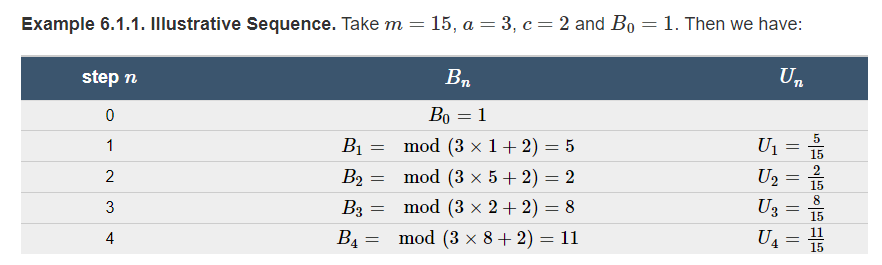
\includegraphics[width=1\linewidth]{images/enamsatu} 

}

\end{figure}

\texttt{Contoh\ 6.1.2.} Menghasilkan Nomor Acak Seragam di \emph{R}. Kode berikut menunjukkan cara menghasilkan tiga angka seragam (0,1) dalam R menggunakan perintah \emph{runif}. Fungsi \emph{set.seed()} di R digunakan untuk membuat hasil yang dapat direproduksi saat menulis kode yang melibatkan pembuatan variabel yang mengambil nilai acak.

\begin{Shaded}
\begin{Highlighting}[]
\FunctionTok{set.seed}\NormalTok{(}\DecValTok{2017}\NormalTok{)}
\NormalTok{U }\OtherTok{\textless{}{-}} \FunctionTok{runif}\NormalTok{(}\DecValTok{3}\NormalTok{)}
\NormalTok{knitr}\SpecialCharTok{::}\FunctionTok{kable}\NormalTok{(U, }\AttributeTok{digits=}\DecValTok{5}\NormalTok{, }\AttributeTok{align =} \StringTok{"c"}\NormalTok{, }\AttributeTok{col.names =} \StringTok{"Uniform"}\NormalTok{)}
\end{Highlighting}
\end{Shaded}

\begin{tabular}{c}
\hline
Uniform\\
\hline
0.92424\\
\hline
0.53718\\
\hline
0.46920\\
\hline
\end{tabular}

\hypertarget{metode-transformasi-invers}{%
\subsection{(6.1.2) Metode Transformasi Invers}\label{metode-transformasi-invers}}

Metode transformasi invers digunakan untuk membangkitkan data acak dari distribusi peluang kontinu yang diketahui bentuk fungsinya.

Dengan urutan bilangan acak seragam, kemudian diubah menjadi distribution of interest (\(F\)).

\[X_i=F^{-1}\left( U_i \right) .\]

\[F^{-1}(y) = \inf_x ~ \{ F(x) \ge y \}\]

\emph{inf} singkatan dari *infimum atau batas bawah terbesar. Ini pada dasarnya adalah nilai \(x\) terkecil yang memenuhi pertidaksamaan \(\{F(x) \ge y\}\). Hasilnya adalah urutan \(X_{i}\) kira-kira iid dengan fungsi distribusi \(F\) jika \(U_{i}\) adalah iid dengan fungsi distribusi seragam ( 0 , 1 ).

\texttt{Contoh\ 6.1.3.} Menghasilkan Bilangan Acak Eksponensial. Misalkan ingin menghasilkan pengamatan dari distribusi eksponensial dengan parameter skala \(θ\) sehingga \(F(x) = 1 - e^{-x/\theta}\). Untuk menghitung transformasi invers, maka dapat menggunakan langkah-langkah berikut:

\[\begin{aligned}
 y = F(x) &\Leftrightarrow  y = 1-e^{-x/\theta} \\
  &\Leftrightarrow -\theta \ln(1-y) = x = F^{-1}(y) .
\end{aligned}\]

Jadi, jika \(U\) memiliki distribusi seragam (0,1), maka \(X = -\theta \ln(1-U)\) memiliki distribusi eksponensial dengan parameter \(θ\).

Seperti pada Contoh 6.1.2 kemudian mengubahnya menjadi variabel acak terdistribusi eksponensial independen dengan rata-rata \(10\). Sebagai alternatif, menggunakan fungsi \emph{rexp} pada R digunakan untuk mensimulasikan sekumpulan bilangan acak yang diambil dari distribusi eksponensial.

\begin{Shaded}
\begin{Highlighting}[]
\FunctionTok{set.seed}\NormalTok{(}\DecValTok{2017}\NormalTok{)}
\NormalTok{U }\OtherTok{\textless{}{-}} \FunctionTok{runif}\NormalTok{(}\DecValTok{3}\NormalTok{)}
\NormalTok{X1 }\OtherTok{\textless{}{-}} \SpecialCharTok{{-}}\DecValTok{10}\SpecialCharTok{*}\FunctionTok{log}\NormalTok{(}\DecValTok{1}\SpecialCharTok{{-}}\NormalTok{U)}
\FunctionTok{set.seed}\NormalTok{(}\DecValTok{2017}\NormalTok{)}
\NormalTok{X2 }\OtherTok{\textless{}{-}} \FunctionTok{rexp}\NormalTok{(}\DecValTok{3}\NormalTok{, }\AttributeTok{rate =} \DecValTok{1}\SpecialCharTok{/}\DecValTok{10}\NormalTok{)}
\end{Highlighting}
\end{Shaded}

\begin{figure}

{\centering 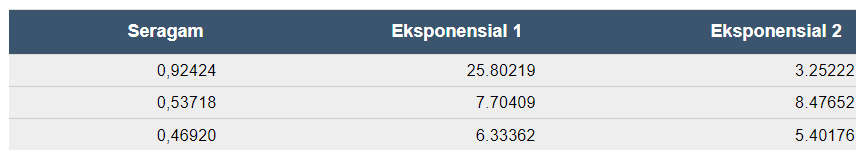
\includegraphics[width=1\linewidth]{images/6.1.2-1} 

}

\end{figure}

\texttt{Contoh\ 6.1.4.} Menghasilkan Angka Acak Pareto. Misalkan ingin menghasilkan pengamatan dari distribusi Pareto dengan parameter \(α\) dan \(θ\) sehingga \(F(x) = 1 - \left(\frac{\theta}{x+\theta} \right)^{\alpha}\). Untuk menghitung transformasi invers, maka dapat menggunakan langkah-langkah berikut:

\[\begin{aligned}
 y = F(x) &\Leftrightarrow 1-y = \left(\frac{\theta}{x+\theta} \right)^{\alpha} \\
  &\Leftrightarrow \left(1-y\right)^{-1/\alpha} = \frac{x+\theta}{\theta} = \frac{x}{\theta} +1 \\
    &\Leftrightarrow \theta \left((1-y)^{-1/\alpha} - 1\right) = x = F^{-1}(y) .\end{aligned}\]

Dengan demikian, \(X = \theta \left((1-U)^{-1/\alpha} - 1\right)\) memiliki distribusi Pareto dengan parameter \(α\) dan \(θ\) .

\texttt{Contoh\ 6.1.5.} Menghasilkan Bilangan Acak Bernoulli. Misalkan ingin mensimulasikan variabel acak dari distribusi Bernoulli dengan parameter \(Q= 0,85\).

\begin{figure}

{\centering 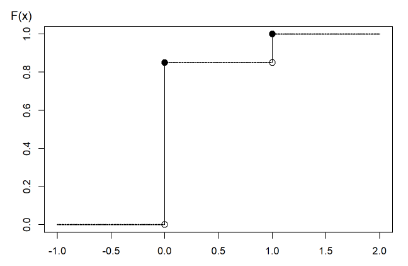
\includegraphics[width=1\linewidth]{images/6.1.2-2} 

}

\end{figure}

Grafik fungsi distribusi kumulatif pada Gambar diatas menunjukkan bahwa fungsi kuantil dapat ditulis sebagai berikut.

\[\begin{aligned}
F^{-1}(y) = \left\{ \begin{array}{cc}
              0 & 0<y \leq 0.85 \\
              1 & 0.85 < y  \leq  1.0 .
            \end{array} \right.
\end{aligned}\]

Jadi, dengan transformasi invers kita dapat mendefinisikan

\[\begin{aligned}
X = \left\{ \begin{array}{cc}
              0 & 0<U \leq 0.85  \\
              1 &  0.85 < U  \leq  1.0
            \end{array} \right.
\end{aligned}\]

Misalnya, ingin menghasilkan tiga angka acak untuk diperoleh

\begin{Shaded}
\begin{Highlighting}[]
\FunctionTok{set.seed}\NormalTok{(}\DecValTok{2017}\NormalTok{)}
\NormalTok{U }\OtherTok{\textless{}{-}} \FunctionTok{runif}\NormalTok{(}\DecValTok{3}\NormalTok{)}
\NormalTok{X }\OtherTok{\textless{}{-}} \DecValTok{1}\SpecialCharTok{*}\NormalTok{(U }\SpecialCharTok{\textgreater{}} \FloatTok{0.85}\NormalTok{)}
\end{Highlighting}
\end{Shaded}

\begin{figure}

{\centering 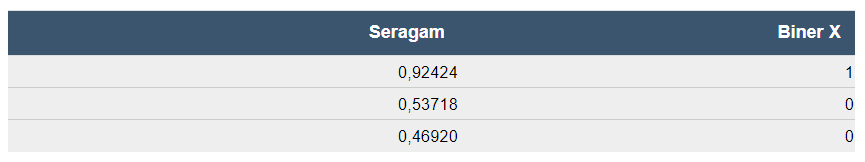
\includegraphics[width=1\linewidth]{images/6.1.2-3} 

}

\end{figure}

\texttt{Contoh\ 6.1.6.} Menghasilkan Angka Acak dari Distribusi Diskrit. Pertimbangkan waktu kegagalan mesin dalam lima tahun pertama. Distribusi waktu kegagalan diberikan sebagai:

\begin{figure}

{\centering 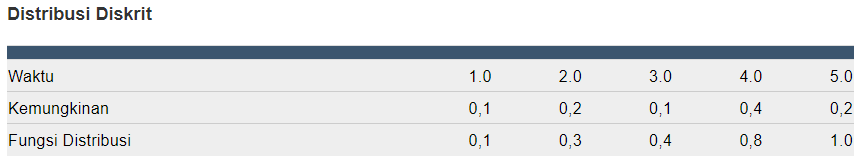
\includegraphics[width=1\linewidth]{images/6.1.2-4} 

}

\end{figure}

\begin{figure}

{\centering 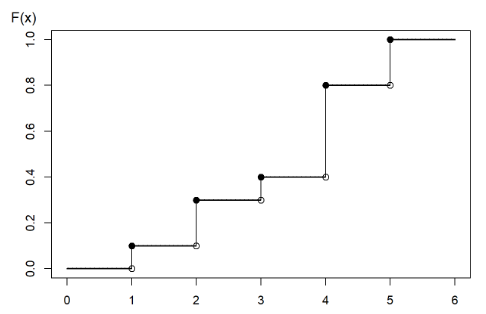
\includegraphics[width=1\linewidth]{images/6.1.2-5} 

}

\end{figure}

Dengan menggunakan grafik fungsi distribusi pada gambar diatas , dengan transformasi invers dapat definisikan

\[\small{
\begin{aligned}
X = \left\{ \begin{array}{cc}
              1 &   0<U  \leq 0.1  \\
              2 &  0.1 < U  \leq  0.3\\
              3 &  0.3 < U  \leq  0.4\\
              4 &  0.4 < U  \leq  0.8  \\
              5 &  0.8 < U  \leq  1.0     .
            \end{array} \right.
\end{aligned}
}\]

Untuk variabel acak diskrit umum mungkin tidak ada urutan hasil. Misalnya, seseorang dapat memiliki salah satu dari lima jenis produk asuransi jiwa dan dapat menggunakan algoritme berikut untuk menghasilkan hasil acak:

\[{\small
\begin{aligned}
X = \left\{ \begin{array}{cc}
  \textrm{whole life} &   0<U  \leq 0.1  \\
 \textrm{endowment} &  0.1 < U  \leq  0.3\\
\textrm{term life} &  0.3 < U  \leq  0.4\\
  \textrm{universal life} &  0.4 < U  \leq  0.8  \\
  \textrm{variable life} &  0.8 < U  \leq  1.0 .
            \end{array} \right.
\end{aligned}
}\]

Analis lain dapat menggunakan prosedur alternatif seperti:

\[{\small
\begin{aligned}
X = \left\{ \begin{array}{cc}
  \textrm{whole life} &   0.9<U<1.0  \\
 \textrm{endowment} &  0.7 \leq U < 0.9\\
\textrm{term life} &  0.6 \leq U < 0.7\\
  \textrm{universal life} &  0.2 \leq U < 0.6  \\
  \textrm{variable life} &  0 \leq U < 0.2 .
            \end{array} \right.
\end{aligned}
}\]

Kedua algoritma menghasilkan (dalam jangka panjang) probabilitas yang sama, misalnya, \(\Pr(\textrm{whole life})=0.1\) , Dan seterusnya. Jadi, tidak ada yang salah ini menunjukkan bahwa ada lebih dari satu cara untuk mencapai suatu tujuan. Demikian pula, dapat menggunakan algoritme alternatif untuk hasil yang diurutkan (seperti waktu kegagalan 1, 2, 3, 4, atau 5, di atas).

\texttt{Contoh\ 6.1.7.} Menghasilkan Angka Acak dari Distribusi Hybrid. Pertimbangkan variabel acak yaitu 0 dengan probabilitas 70\% dan terdistribusi secara eksponensial dengan parameter \(\theta= 10,000\) dengan probabilitas 30\%. Dalam aplikasi asuransi, ini mungkin sesuai dengan peluang 70\% tidak memiliki klaim asuransi dan peluang klaim 30\% - jika klaim terjadi, maka itu didistribusikan secara eksponensial. Fungsi distribusi, digambarkan pada gambar dibawah ini , diberikan sebagai

\[\begin{aligned}
F(y) = \left\{ \begin{array}{cc}
              0 &  x<0  \\
              1 - 0.3 \exp(-x/10000) & x \ge 0 .
            \end{array} \right.
\end{aligned}\]

\begin{figure}

{\centering 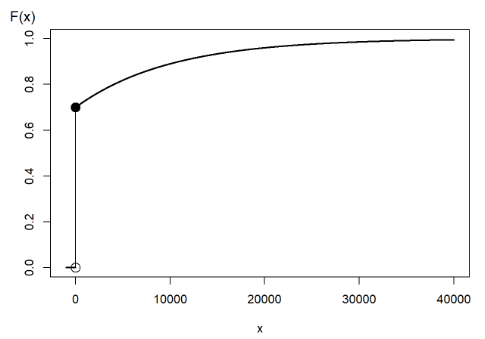
\includegraphics[width=1\linewidth]{images/6.1.2-6} 

}

\end{figure}

Dari Gambar diatas dapat dilihat bahwa transformasi invers untuk membangkitkan variabel acak dengan fungsi distribusi ini adalah

\[\begin{aligned}
X = F^{-1}(U) = \left\{ \begin{array}{cc}
              0 &  0< U  \leq  0.7  \\
              -1000 \ln (\frac{1-U}{0.3}) & 0.7 < U < 1 .
            \end{array} \right.
\end{aligned}\]

\hypertarget{presisi-simulasi}{%
\subsection{(6.1.3) Presisi Simulasi}\label{presisi-simulasi}}

Setelah mengetahui cara menghasilkan realisasi simulasi independen dari distribusi bunga, maka dapat menyusun distribusi empiris (distribusi empiris mengelompokkan data ke dalam suatu interval, di mana frekuensi data dalam setiap interval dapat digunakan untuk menentukan frekuensi relatifnya) dan memperkirakan distribusi yang diperlukan.

Banyak dari aplikasi ini dapat direduksi menjadi masalah perkiraan \(\mathrm{E~}[h(X)]\) , Di mana \(h(\cdot)\) adalah beberapa fungsi yang diketahui. Berdasarkan simulasi R (replikasi), sehingga didapatkan \(X_1,\ldots,X_R\). Dari sampel yang disimulasikan ini, dapat menghitung rata-rata sebagai berikut.

\[\overline{h}_R=\frac{1}{R}\sum_{i=1}^{R} h(X_i)\]

sebagai perkiraan simulasi dari \(\mathrm{E~}[h(X)]\). Untuk memperkirakan ketepatan perkiraan tersebut, maka menggunakan varians simulasi

\[s_{h,R}^2 = \frac{1}{R-1} \sum_{i=1}^{R}\left( h(X_i) -\overline{h}_R
\right) ^2.\]

Dari independensi, kesalahan standar estimasi adalah \(s_{h,R}/\sqrt{R}\). Kesalahan standar estimasi dapat dibuat sekecil dengan meningkatkan jumlah replikasi \(R\).

\texttt{Contoh\ 6.1.8.} Manajemen portofolio. Pada Bagian 3.4 telah mempelajari cara menghitung nilai ekspektasi polis dengan deductible. Sebagai contoh dari sesuatu yang tidak dapat dilakukan dengan ekspresi bentuk tertutup, kemudian akan mempertimbangkan dua risiko. (Ini adalah variasi dari contoh yang lebih kompleks yang akan dibahas sebagai Contoh 10.3.6).

Dengan mempertimbangkan dua risiko properti dari perusahaan telekomunikasi:

\begin{itemize}
\item
  \(X_1\) - bangunan, dimodelkan menggunakan distribusi gamma dengan rata-rata 200 dan parameter skala 100.
\item
  \(X_2\) - kendaraan bermotor, dimodelkan menggunakan distribusi gamma dengan mean 400 dan parameter skala 200.
\end{itemize}

Nyatakan risiko total sebagai \(X = X_1 + X_2\). Untuk penyederhanaan, dapat diasumsikan bahwa risiko ini tidak bergantung.

Untuk mengelola risiko maka diperlukan perlindungan atau penjamin asuransi dan bersedia mempertahankan jumlah bangunan dan kendaraan bermotor kecil secara internal, hingga \(M\). Jumlah acak lebih dari \(M\) akan memiliki pengaruh yang tidak terduga pada anggaran dan karenanya untuk jumlah ini dapat mencari perlindungan asuransi. Dinyatakan secara matematis, risiko yang dipertahankan adalah \(Y_{retained}=\min(X_1 + X_2,M)\) dan bagian penanggung adalah \(Y_{insurer} = X- Y_{retained}\).

Misalnya \(M= 400\) serta \(R = 1000000\).

\texttt{A.} Dengan pengaturan tersebut, ingin menentukan perkiraan jumlah klaim dan standar deviasi terkait dari (i) yang ditahan, (ii) yang diterima oleh perusahaan asuransi, dan (iii) total jumlah keseluruhan.

\begin{Shaded}
\begin{Highlighting}[]
\CommentTok{\# Simulate the risks}
\NormalTok{nSim }\OtherTok{\textless{}{-}} \FloatTok{1e6}  \CommentTok{\#number of simulations}
\FunctionTok{set.seed}\NormalTok{(}\DecValTok{2017}\NormalTok{) }\CommentTok{\#set seed to reproduce work }
\NormalTok{X1 }\OtherTok{\textless{}{-}} \FunctionTok{rgamma}\NormalTok{(nSim ,alpha1,}\AttributeTok{scale =}\NormalTok{ theta1)  }
\NormalTok{X2 }\OtherTok{\textless{}{-}} \FunctionTok{rgamma}\NormalTok{(nSim ,alpha2,}\AttributeTok{scale =}\NormalTok{ theta2) }

\CommentTok{\# Portfolio Risks}
\NormalTok{X         }\OtherTok{\textless{}{-}}\NormalTok{ X1 }\SpecialCharTok{+}\NormalTok{ X2 }
\NormalTok{Yretained }\OtherTok{\textless{}{-}} \FunctionTok{pmin}\NormalTok{(X, M)}
\NormalTok{Yinsurer  }\OtherTok{\textless{}{-}}\NormalTok{ X }\SpecialCharTok{{-}}\NormalTok{ Yretained}
\end{Highlighting}
\end{Shaded}

Kemudian jumlah klaim yang diharapkan adalah

\begin{Shaded}
\begin{Highlighting}[]
\CommentTok{\# Expected Claim Amounts}
\NormalTok{ExpVec }\OtherTok{\textless{}{-}} \FunctionTok{t}\NormalTok{(}\FunctionTok{as.matrix}\NormalTok{(}\FunctionTok{c}\NormalTok{(}\FunctionTok{mean}\NormalTok{(Yretained),}\FunctionTok{mean}\NormalTok{(Yinsurer),}\FunctionTok{mean}\NormalTok{(X))))}
\NormalTok{sdVec }\OtherTok{\textless{}{-}} \FunctionTok{t}\NormalTok{(}\FunctionTok{as.matrix}\NormalTok{(}\FunctionTok{c}\NormalTok{(}\FunctionTok{sd}\NormalTok{(Yretained),}\FunctionTok{sd}\NormalTok{(Yinsurer),}\FunctionTok{sd}\NormalTok{(X))))}
\NormalTok{outMat }\OtherTok{\textless{}{-}} \FunctionTok{rbind}\NormalTok{(ExpVec, sdVec)}
\FunctionTok{colnames}\NormalTok{(outMat) }\OtherTok{\textless{}{-}} \FunctionTok{c}\NormalTok{(}\StringTok{"Retained"}\NormalTok{, }\StringTok{"Insurer"}\NormalTok{,}\StringTok{"Total"}\NormalTok{)}
\FunctionTok{row.names}\NormalTok{(outMat) }\OtherTok{\textless{}{-}} \FunctionTok{c}\NormalTok{(}\StringTok{"Mean"}\NormalTok{,}\StringTok{"Standard Deviation"}\NormalTok{)}
\FunctionTok{round}\NormalTok{(outMat,}\AttributeTok{digits=}\DecValTok{2}\NormalTok{)}
\end{Highlighting}
\end{Shaded}

\begin{figure}

{\centering 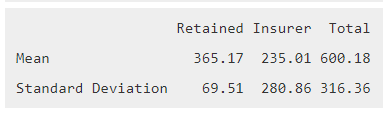
\includegraphics[width=1\linewidth]{images/6.1.3-1} 

}

\end{figure}

\texttt{B.} Untuk klaim yang diasuransikan, kesalahan standar perkiraan simulasi adalah \(s_{h,R}/\sqrt{1000000} =/\sqrt{1000000} =0.281\). Untuk contoh ini, simulasi cepat dan nilai yang besar seperti 1000000 adalah pilihan yang mudah. Namun, untuk masalah yang lebih kompleks, ukuran simulasi mungkin menjadi masalah.

\begin{Shaded}
\begin{Highlighting}[]
\NormalTok{Yinsurefct }\OtherTok{\textless{}{-}} \ControlFlowTok{function}\NormalTok{(numSim)\{}
\NormalTok{X1 }\OtherTok{\textless{}{-}} \FunctionTok{rgamma}\NormalTok{(numSim,alpha1,}\AttributeTok{scale =}\NormalTok{ theta1)  }
\NormalTok{X2 }\OtherTok{\textless{}{-}} \FunctionTok{rgamma}\NormalTok{(numSim,alpha2,}\AttributeTok{scale =}\NormalTok{ theta2)  }
\CommentTok{\# Portfolio Risks}
\NormalTok{X         }\OtherTok{\textless{}{-}}\NormalTok{ X1 }\SpecialCharTok{+}\NormalTok{ X2 }
\NormalTok{Yinsurer }\OtherTok{\textless{}{-}}\NormalTok{ X }\SpecialCharTok{{-}} \FunctionTok{pmin}\NormalTok{(X, M)}
\FunctionTok{return}\NormalTok{(Yinsurer)}
\NormalTok{\}}
\NormalTok{R }\OtherTok{\textless{}{-}} \FloatTok{1e3}
\NormalTok{nPath }\OtherTok{\textless{}{-}} \DecValTok{20}
\FunctionTok{set.seed}\NormalTok{(}\DecValTok{2017}\NormalTok{)}
\NormalTok{simU }\OtherTok{\textless{}{-}} \FunctionTok{matrix}\NormalTok{(}\FunctionTok{Yinsurefct}\NormalTok{(R}\SpecialCharTok{*}\NormalTok{nPath),R,nPath)}
\NormalTok{sumP2 }\OtherTok{\textless{}{-}} \FunctionTok{apply}\NormalTok{(simU, }\DecValTok{2}\NormalTok{, cumsum)}\SpecialCharTok{/}\NormalTok{(}\DecValTok{1}\SpecialCharTok{:}\NormalTok{R)}
\end{Highlighting}
\end{Shaded}

\begin{Shaded}
\begin{Highlighting}[]
\FunctionTok{matplot}\NormalTok{(}\DecValTok{1}\SpecialCharTok{:}\NormalTok{R,sumP2[,}\DecValTok{1}\SpecialCharTok{:}\DecValTok{20}\NormalTok{],}\AttributeTok{type=}\StringTok{"l"}\NormalTok{,}\AttributeTok{col=}\FunctionTok{rgb}\NormalTok{(}\DecValTok{1}\NormalTok{,}\DecValTok{0}\NormalTok{,}\DecValTok{0}\NormalTok{,.}\DecValTok{2}\NormalTok{), }\AttributeTok{ylim=}\FunctionTok{c}\NormalTok{(}\DecValTok{100}\NormalTok{, }\DecValTok{400}\NormalTok{),}
        \AttributeTok{xlab=}\FunctionTok{expression}\NormalTok{(}\FunctionTok{paste}\NormalTok{(}\StringTok{"Number of Simulations ("}\NormalTok{, }\FunctionTok{italic}\NormalTok{(}\StringTok{\textquotesingle{}R\textquotesingle{}}\NormalTok{), }\StringTok{")"}\NormalTok{)), }
        \AttributeTok{ylab=}\StringTok{"Expected Insurer Claims"}\NormalTok{)}
\FunctionTok{abline}\NormalTok{(}\AttributeTok{h=}\FunctionTok{mean}\NormalTok{(Yinsurer),}\AttributeTok{lty=}\DecValTok{2}\NormalTok{)}
\NormalTok{bonds }\OtherTok{\textless{}{-}} \FunctionTok{cbind}\NormalTok{(}\FloatTok{1.96}\SpecialCharTok{*}\FunctionTok{sd}\NormalTok{(Yinsurer)}\SpecialCharTok{*}\FunctionTok{sqrt}\NormalTok{(}\DecValTok{1}\SpecialCharTok{/}\NormalTok{(}\DecValTok{1}\SpecialCharTok{:}\NormalTok{R)),}\SpecialCharTok{{-}}\FloatTok{1.96}\SpecialCharTok{*}\FunctionTok{sd}\NormalTok{(Yinsurer)}\SpecialCharTok{*}\FunctionTok{sqrt}\NormalTok{(}\DecValTok{1}\SpecialCharTok{/}\NormalTok{(}\DecValTok{1}\SpecialCharTok{:}\NormalTok{R)))}
\FunctionTok{matlines}\NormalTok{(}\DecValTok{1}\SpecialCharTok{:}\NormalTok{R,bonds}\SpecialCharTok{+}\FunctionTok{mean}\NormalTok{(Yinsurer),}\AttributeTok{col=}\StringTok{"red"}\NormalTok{,}\AttributeTok{lty=}\DecValTok{1}\NormalTok{)}
\end{Highlighting}
\end{Shaded}

\begin{figure}

{\centering 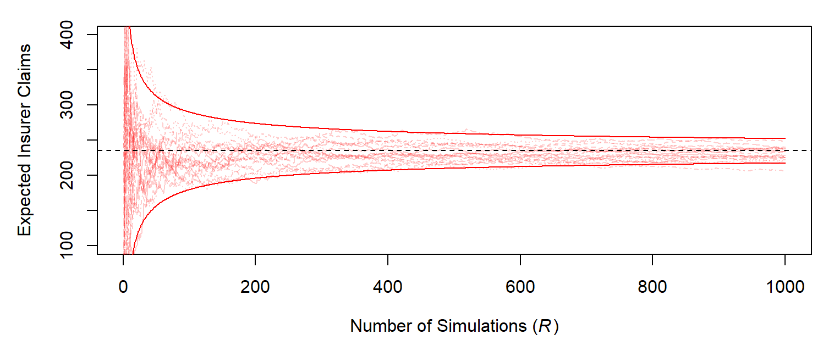
\includegraphics[width=1\linewidth]{images/6.1.3-2} 

}

\end{figure}

Dari grafik diatas dapat dilihat, semakin banyak jumlah simulasi R maka semakin sedikit jumlah klaim yang diharapkan.

\texttt{Penentuan\ Jumlah\ Simulasi}

Misalkan ingin berada dalam 1\% dari rata-rata dengan kepastian 95\%. Artinya, \(\Pr \left( |\overline{h}_R - \mathrm{E~}[h(X)]| \le 0.01 \mathrm{E~}[h(X)] \right) \ge 0.95\). Menurut teorema limit pusat, perkiraan harus terdistribusi secara normal dan mengharapkan R cukup besar untuk \(0.01 \mathrm{E~}[h(X)]/\sqrt{\mathrm{Var~}[h(X)]/R}) \ge 1.96\) . (Ingat bahwa 1,96 adalah persentil ke-97,5 dari distribusi normal standar.) Mengganti \(\mathrm{E~}[h(X)]\) Dan \(\mathrm{Var~}[h(X)]\) dengan estimasi,sehingga

\[\frac{.01\overline{h}_R}{s_{h,R}/\sqrt{R}}\geq 1.96\]

\[\begin{equation}
R \geq 38,416\frac{s_{h,R}^2}{\overline{h}_R^2}.
\tag{6.1}
\end{equation}\]

\texttt{Contoh\ 6.1.9.} Pilihan Perkiraan.

Sebuah aplikasi penting dari simulasi adalah pendekatan dari \(\mathrm{E~}[h(X)]\). Dalam contoh ini, kami menunjukkan bahwa pilihan dari \(h(\cdot)\) fungsi dan distribusi \(X\) dapat berperan.

Pertimbangkan pertanyaan berikut: apa itu \(\Pr[X>2]\). Kapan \(X\) mempunyai sebuah distribusi Cauchy (distribusi probabilitas kontinu), dengan fungsi kepadatan \(f(x) =\left(\pi(1+x^2)\right)^{-1}\), pada garis sebenarnya? Nilai sebenarnya adalah

\[\Pr\left[X>2\right] = \int_2^\infty \frac{dx}{\pi(1+x^2)} .\]

\begin{Shaded}
\begin{Highlighting}[]
\NormalTok{true\_value }\OtherTok{\textless{}{-}} \FunctionTok{integrate}\NormalTok{(}\ControlFlowTok{function}\NormalTok{(x) }\DecValTok{1}\SpecialCharTok{/}\NormalTok{(pi}\SpecialCharTok{*}\NormalTok{(}\DecValTok{1}\SpecialCharTok{+}\NormalTok{x}\SpecialCharTok{\^{}}\DecValTok{2}\NormalTok{)),}\AttributeTok{lower=}\DecValTok{2}\NormalTok{,}\AttributeTok{upper=}\ConstantTok{Inf}\NormalTok{)}\SpecialCharTok{$}\NormalTok{value}
\NormalTok{true\_value }
\end{Highlighting}
\end{Shaded}

\begin{verbatim}
## [1] 0.1475836
\end{verbatim}

\texttt{Perkiraan\ 1.} Sebagai alternatif, seseorang dapat menggunakan teknik simulasi untuk memperkirakan besaran tersebut. Dari kalkulus, dapat memeriksa bahwa fungsi kuantil dari distribusi Cauchy adalah \(F^{-1}(y) = \tan \left( \pi(y-0.5) \right)\) . Kemudian, dengan variasi seragam (0,1) yang disimulasikan, \(U_1, \ldots, U_R\), sehingga dapat membangun estimator

\begin{Shaded}
\begin{Highlighting}[]
\NormalTok{Q }\OtherTok{\textless{}{-}} \ControlFlowTok{function}\NormalTok{(u) }\FunctionTok{tan}\NormalTok{(pi}\SpecialCharTok{*}\NormalTok{(u}\FloatTok{{-}.5}\NormalTok{))}
\NormalTok{R }\OtherTok{\textless{}{-}} \FloatTok{1e6}
\FunctionTok{set.seed}\NormalTok{(}\DecValTok{1}\NormalTok{)}
\NormalTok{X }\OtherTok{\textless{}{-}} \FunctionTok{Q}\NormalTok{(}\FunctionTok{runif}\NormalTok{(R))}
\NormalTok{p1 }\OtherTok{\textless{}{-}} \FunctionTok{mean}\NormalTok{(X}\SpecialCharTok{\textgreater{}}\DecValTok{2}\NormalTok{)}
\NormalTok{se.p1 }\OtherTok{\textless{}{-}} \FunctionTok{sd}\NormalTok{(X}\SpecialCharTok{\textgreater{}}\DecValTok{2}\NormalTok{)}\SpecialCharTok{/}\FunctionTok{sqrt}\NormalTok{(R)}
\NormalTok{p1}
\end{Highlighting}
\end{Shaded}

\begin{verbatim}
## [1] 0.147439
\end{verbatim}

\begin{Shaded}
\begin{Highlighting}[]
\NormalTok{se.p1}
\end{Highlighting}
\end{Shaded}

\begin{verbatim}
## [1] 0.0003545432
\end{verbatim}

Dengan satu juta simulasi, diperoleh estimasi sebesar 0,14744 dengan standard error 0,355 (dibagi 1000). Dapat dibuktikan bahwa varian dari \(P_1\) teratur \(0.127/R\).

\texttt{Perkiraan\ 2.} Dengan pilihan lain dari \(h(\cdot)\) Dan \(f(\cdot)\) adalah mungkin untuk mengurangi ketidakpastian bahkan dengan menggunakan jumlah simulasi yang sama \(R\) . Untuk memulai, seseorang dapat menggunakan simetri distribusi Cauchy untuk menulis \(\Pr[X>2]=0.5\cdot\Pr[|X|>2]\) . Dengan ini, dapat membuat estimator baru

\[p_2 = \frac{1}{2R}\sum_{i=1}^R \mathrm{I}(|F^{-1}(U_i)|>2) .\]

Dengan satu juta simulasi, diperoleh estimasi sebesar 0,14748 dengan standard error 0,228 (dibagi 1000). Dapat dibuktikan bahwa varian dari \(P_2\) teratur \(0.052/R\).

\texttt{Perkiraan\ 3.} Integral tak wajar dapat ditulis dengan sifat simetri sederhana (karena fungsinya simetris dan integral pada garis real sama dengan 1 ).

\[\int_2^\infty \frac{dx}{\pi(1+x^2)}=\frac{1}{2}-\int_0^2\frac{dx}{\pi(1+x^2)} .\]

\[p_3 = \frac{1}{2}-\frac{1}{R}\sum_{i=1}^R h_3(2U_i), ~~~~~~\text{where}~h_3(x)=\frac{2}{\pi(1+x^2)} .\]

Dengan satu juta simulasi, diperoleh estimasi sebesar 0,14756 dengan standard error 0,169 (dibagi 1000). Dapat dibuktikan bahwa varian dari \(P_3\) teratur \(0,0285 / R\).

\texttt{Perkiraan\ 4.} Akhirnya, seseorang juga dapat mempertimbangkan beberapa perubahan variabel dalam integral.

\[\int_2^\infty \frac{dx}{\pi(1+x^2)}=\int_0^{1/2}\frac{y^{-2}dy}{\pi(1-y^{-2})} .\]

\[p_4 = \frac{1}{R}\sum_{i=1}^R h_4(U_i/2),~~~~~\text{where}~h_4(x)=\frac{1}{2\pi(1+x^2)} .\]

Dengan satu juta simulasi, diperoleh estimasi sebesar 0,14759 dengan standard error 0,01 (dibagi 1000). Dapat dibuktikan bahwa varian dari \(P_4\) teratur \(0,00009 / R\) , yang jauh lebih kecil dari yang lainnya.

Tabel berikut merupakan rangkuman dari empat pilihan \(h(\cdot)\) Dan \(f(\cdot)\)) untuk memperkirakan \(\Pr[X>2] = 0,14758\). Kesalahan standar bervariasi. Jadi, jika memiliki tingkat akurasi yang diinginkan, maka jumlah simulasi sangat bergantung pada bagaimana menulis integral yang akan diaproksimasi.

\begin{figure}

{\centering 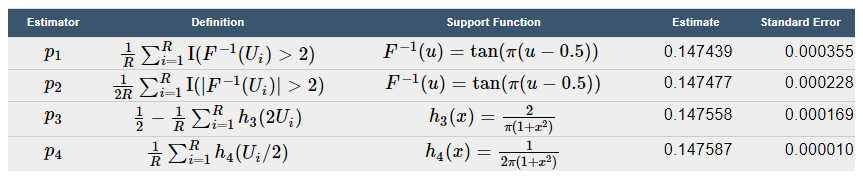
\includegraphics[width=1\linewidth]{images/6.1.3-3} 

}

\end{figure}

\hypertarget{imulasi-dan-inferensi-statistik}{%
\subsection{(6.1.4) imulasi dan Inferensi Statistik}\label{imulasi-dan-inferensi-statistik}}

Simulasi tidak hanya membantu dalam memperkirakan nilai yang diharapkan tetapi juga berguna dalam menghitung aspek lain dari fungsi distribusi. Secara khusus, ini sangat berguna ketika distribusi statistik uji terlalu rumit untuk diturunkan. Dalam hal ini, seseorang dapat menggunakan simulasi untuk memperkirakan distribusi referensi.

\texttt{Contoh\ 6.1.10.} Uji Distribusi Kolmogorov-Smirnov.

Misalkan terdapata \(n = 100\) observasi \(\{x_1,\cdots,x_n\}\) yang, tidak diketahui oleh analis, dihasilkan dari distribusi gamma dengan parameter \(\alpha = 6\) Dan \(\theta=2\) . Analis percaya bahwa data berasal dari distribusi lognormal dengan parameter 1 dan 0,4 dan ingin menguji asumsi ini.

\begin{Shaded}
\begin{Highlighting}[]
\FunctionTok{set.seed}\NormalTok{(}\DecValTok{1}\NormalTok{)}
\NormalTok{n }\OtherTok{\textless{}{-}} \DecValTok{100}
\NormalTok{x }\OtherTok{\textless{}{-}} \FunctionTok{rgamma}\NormalTok{(n, }\DecValTok{6}\NormalTok{, }\DecValTok{2}\NormalTok{)}

\NormalTok{u}\OtherTok{=}\FunctionTok{seq}\NormalTok{(}\DecValTok{0}\NormalTok{,}\DecValTok{7}\NormalTok{,}\AttributeTok{by=}\NormalTok{.}\DecValTok{01}\NormalTok{)}
\NormalTok{vx }\OtherTok{=} \FunctionTok{c}\NormalTok{(}\DecValTok{0}\NormalTok{,}\FunctionTok{sort}\NormalTok{(x))}
\NormalTok{vy }\OtherTok{=}\NormalTok{ (}\DecValTok{0}\SpecialCharTok{:}\NormalTok{n)}\SpecialCharTok{/}\NormalTok{n}
\end{Highlighting}
\end{Shaded}

\begin{Shaded}
\begin{Highlighting}[]
\FunctionTok{par}\NormalTok{(}\AttributeTok{mfrow=}\FunctionTok{c}\NormalTok{(}\DecValTok{1}\NormalTok{,}\DecValTok{2}\NormalTok{))}
\FunctionTok{hist}\NormalTok{(x,}\AttributeTok{probability =} \ConstantTok{TRUE}\NormalTok{,}\AttributeTok{main=}\StringTok{"Histogram"}\NormalTok{, }\AttributeTok{col=}\StringTok{"light blue"}\NormalTok{,}
     \AttributeTok{border=}\StringTok{"white"}\NormalTok{,}\AttributeTok{xlim=}\FunctionTok{c}\NormalTok{(}\DecValTok{0}\NormalTok{,}\DecValTok{7}\NormalTok{),}\AttributeTok{ylim=}\FunctionTok{c}\NormalTok{(}\DecValTok{0}\NormalTok{,.}\DecValTok{4}\NormalTok{))}
\FunctionTok{lines}\NormalTok{(u,}\FunctionTok{dlnorm}\NormalTok{(u,}\DecValTok{1}\NormalTok{,.}\DecValTok{4}\NormalTok{),}\AttributeTok{col=}\StringTok{"red"}\NormalTok{,}\AttributeTok{lty=}\DecValTok{2}\NormalTok{)}
\FunctionTok{plot}\NormalTok{(vx,vy,}\AttributeTok{type=}\StringTok{"l"}\NormalTok{,}\AttributeTok{xlab=}\StringTok{"x"}\NormalTok{,}\AttributeTok{ylab=}\StringTok{"Cumulative Distribution"}\NormalTok{,}\AttributeTok{main=}\StringTok{"Empirical cdf"}\NormalTok{)}
\FunctionTok{lines}\NormalTok{(u,}\FunctionTok{plnorm}\NormalTok{(u,}\DecValTok{1}\NormalTok{,.}\DecValTok{4}\NormalTok{),}\AttributeTok{col=}\StringTok{"red"}\NormalTok{,}\AttributeTok{lty=}\DecValTok{2}\NormalTok{)}
\end{Highlighting}
\end{Shaded}

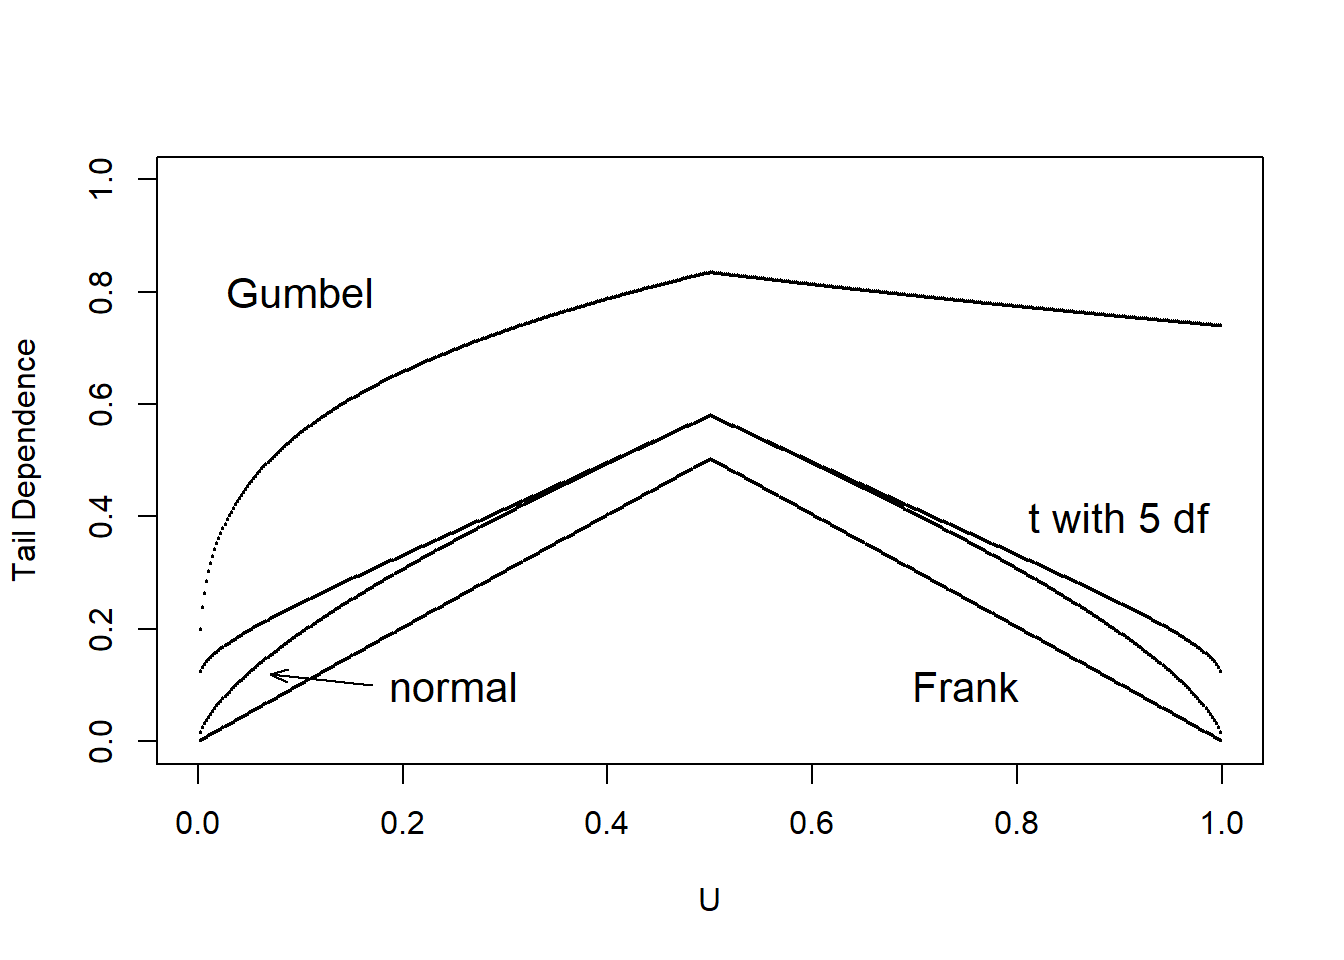
\includegraphics{Analisa_Resiko_files/figure-latex/unnamed-chunk-11-1.pdf}

Dari grafik diatas dapat dilihat bahwa garis putus-putus merah tersebut sesuai dengan distribusi lognormal yang dihipotesiskan.

Perlu digaris bawahi bahwa statistik Kolmogorov-Smirnov sama dengan perbedaan terbesar antara distribusi empiris dan hipotesis. Ini \(\max_x |F_n(x)-F_0(x)|\), Di mana \(F_0\) adalah distribusi lognormal yang dihipotesiskan, sehingga

\begin{Shaded}
\begin{Highlighting}[]
\CommentTok{\# test statistic}
\NormalTok{D }\OtherTok{\textless{}{-}} \ControlFlowTok{function}\NormalTok{(data, F0)\{}
\NormalTok{   F }\OtherTok{\textless{}{-}} \FunctionTok{Vectorize}\NormalTok{(}\ControlFlowTok{function}\NormalTok{(x) }\FunctionTok{mean}\NormalTok{((data}\SpecialCharTok{\textless{}=}\NormalTok{x)))}
\NormalTok{   n }\OtherTok{\textless{}{-}} \FunctionTok{length}\NormalTok{(data)}
\NormalTok{   x }\OtherTok{\textless{}{-}} \FunctionTok{sort}\NormalTok{(data)}
\NormalTok{   d1}\OtherTok{=}\FunctionTok{abs}\NormalTok{(}\FunctionTok{F}\NormalTok{(x}\FloatTok{+1e{-}6}\NormalTok{)}\SpecialCharTok{{-}}\FunctionTok{F0}\NormalTok{(x}\FloatTok{+1e{-}6}\NormalTok{))}
\NormalTok{   d2}\OtherTok{=}\FunctionTok{abs}\NormalTok{(}\FunctionTok{F}\NormalTok{(x}\FloatTok{{-}1e{-}6}\NormalTok{)}\SpecialCharTok{{-}}\FunctionTok{F0}\NormalTok{(x}\FloatTok{{-}1e{-}6}\NormalTok{))}
   \FunctionTok{return}\NormalTok{(}\FunctionTok{max}\NormalTok{(}\FunctionTok{c}\NormalTok{(d1,d2)))}
\NormalTok{\}}
\FunctionTok{D}\NormalTok{(x,}\ControlFlowTok{function}\NormalTok{(x) }\FunctionTok{plnorm}\NormalTok{(x,}\DecValTok{1}\NormalTok{,.}\DecValTok{4}\NormalTok{))}
\end{Highlighting}
\end{Shaded}

\begin{verbatim}
## [1] 0.09703627
\end{verbatim}

\begin{Shaded}
\begin{Highlighting}[]
\FunctionTok{ks.test}\NormalTok{(x, plnorm, }\AttributeTok{mean=}\DecValTok{1}\NormalTok{, }\AttributeTok{sd=}\FloatTok{0.4}\NormalTok{)}
\end{Highlighting}
\end{Shaded}

\begin{verbatim}
## 
##  Asymptotic one-sample Kolmogorov-Smirnov test
## 
## data:  x
## D = 0.097037, p-value = 0.3031
## alternative hypothesis: two-sided
\end{verbatim}

Secara khusus, untuk menghitung P-value, maka hasilkan ribuan sampel acak dari \(LN(1,0.4)\) distribusi (dengan ukuran yang sama), dan menghitung secara empiris distribusi statistik,

\begin{Shaded}
\begin{Highlighting}[]
\NormalTok{ns }\OtherTok{\textless{}{-}} \FloatTok{1e4}
\NormalTok{d\_KS }\OtherTok{\textless{}{-}} \FunctionTok{rep}\NormalTok{(}\ConstantTok{NA}\NormalTok{,ns)}
\CommentTok{\# compute the test statistics for a large (ns) number of simulated samples}
\ControlFlowTok{for}\NormalTok{(s }\ControlFlowTok{in} \DecValTok{1}\SpecialCharTok{:}\NormalTok{ns) d\_KS[s] }\OtherTok{\textless{}{-}} \FunctionTok{D}\NormalTok{(}\FunctionTok{rlnorm}\NormalTok{(n,}\DecValTok{1}\NormalTok{,.}\DecValTok{4}\NormalTok{),}\ControlFlowTok{function}\NormalTok{(x) }\FunctionTok{plnorm}\NormalTok{(x,}\DecValTok{1}\NormalTok{,.}\DecValTok{4}\NormalTok{))}

\FunctionTok{mean}\NormalTok{(d\_KS}\SpecialCharTok{\textgreater{}}\FunctionTok{D}\NormalTok{(x,}\ControlFlowTok{function}\NormalTok{(x) }\FunctionTok{plnorm}\NormalTok{(x,}\DecValTok{1}\NormalTok{,.}\DecValTok{4}\NormalTok{)))}
\end{Highlighting}
\end{Shaded}

\begin{verbatim}
## [1] 0.2843
\end{verbatim}

\begin{Shaded}
\begin{Highlighting}[]
\FunctionTok{hist}\NormalTok{(d\_KS,}\AttributeTok{probability =} \ConstantTok{TRUE}\NormalTok{,}\AttributeTok{col=}\StringTok{"light blue"}\NormalTok{,}\AttributeTok{border=}\StringTok{"white"}\NormalTok{,}\AttributeTok{xlab=}\StringTok{"Test Statistic"}\NormalTok{,}\AttributeTok{main=}\StringTok{""}\NormalTok{)}
\FunctionTok{lines}\NormalTok{(}\FunctionTok{density}\NormalTok{(d\_KS),}\AttributeTok{col=}\StringTok{"red"}\NormalTok{)}
\FunctionTok{abline}\NormalTok{(}\AttributeTok{v=}\FunctionTok{D}\NormalTok{(x,}\ControlFlowTok{function}\NormalTok{(x) }\FunctionTok{plnorm}\NormalTok{(x,}\DecValTok{1}\NormalTok{,.}\DecValTok{4}\NormalTok{)),}\AttributeTok{lty=}\DecValTok{2}\NormalTok{,}\AttributeTok{col=}\StringTok{"red"}\NormalTok{)}
\end{Highlighting}
\end{Shaded}

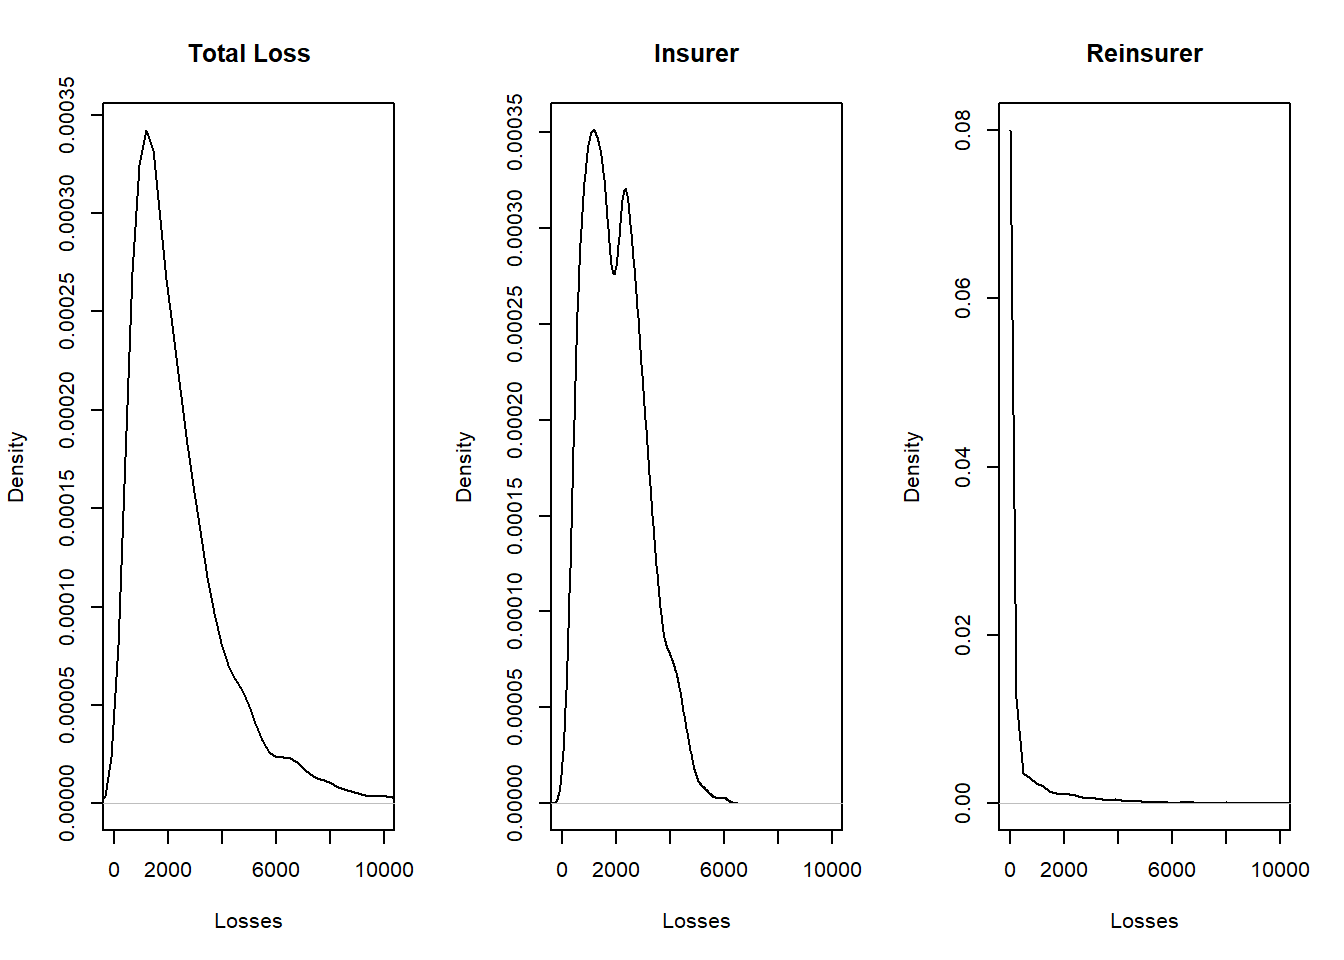
\includegraphics{Analisa_Resiko_files/figure-latex/unnamed-chunk-15-1.pdf}

Distribusi yang disimulasikan berdasarkan 10.000 sampel acak dirangkum grafik diatas. Di sini, statistik melebihi nilai empiris (0,09704) dalam 28,43\%, sedangkan P-value adalah 0,3031. Baik untuk simulasi maupun teoretis P-value, kesimpulannya adalah data tidak memberikan bukti yang cukup untuk menolak hipotesis distribusi lognormal.

Meskipun hanya perkiraan, pendekatan simulasi bekerja dalam berbagai distribusi dan uji statistik tanpa perlu mengembangkan nuansa teori yang mendasari untuk setiap situasi. Berikut ringkasan prosedur untuk mengembangkan distribusi simulasi dan p-value sebagai berikut:

\begin{enumerate}
\def\labelenumi{\arabic{enumi}.}
\item
  Gambarlah sampel berukuran n , katakanlah, \(X_1, \ldots, X_n\), dari fungsi distribusi yang diketahui \(F\). Hitung statistik minat, dilambangkan sebagai \(\hat{\theta}(X_1, \ldots, X_n)\). Panggil ini \(\hat{\theta}^r\) untuk replikasi ke -r .
\item
  Ulangi ini \(r=1, \ldots, R\) kali untuk mendapatkan sampel statistik, \(\hat{\theta}^1, \ldots,\hat{\theta}^R\).
\item
  Dari sampel statistik pada Langkah 2, \(\{\hat{\theta}^1, \ldots,\hat{\theta}^R\}\), hitung ukuran ringkasan minat, seperti p-value.
\end{enumerate}

\hypertarget{bootstrap-dan-resampling}{%
\section{(6.2) Bootstrap dan Resampling}\label{bootstrap-dan-resampling}}

Subbab ini akan mempelajari :

\begin{enumerate}
\def\labelenumi{\arabic{enumi}.}
\item
  Hasilkan distribusi bootstrap nonparametrik untuk statistik minat
\item
  Gunakan distribusi bootstrap untuk menghasilkan estimasi presisi untuk statistik yang diminati, termasuk bias, standar deviasi, dan interval kepercayaan
\item
  Lakukan analisis bootstrap untuk distribusi parametrik
\end{enumerate}

\hypertarget{dasar-dasar-bootstrap}{%
\subsection{(6.2.1) Dasar-dasar Bootstrap}\label{dasar-dasar-bootstrap}}

Metode bootstrap adalah metode berbasis resampling data sampel dengan syarat pengembalian pada datanya dalam menyelesaikan statistik ukuran suatu sampel dengan harapan sampel tersebut mewakili data populai sebenarnya, biasanya ukuran resampling diambil secara ribuan kali agar dapat mewakili data populasinya. Algoritma resamplign umum dengan \(\{X_1, \ldots, X_n\}\) untuk menunjukkan sampel asli dan \(\{X_1^*, \ldots, X_n^*\}\) menunjukkan undian yang disimulasikan.

Untuk setiap sampel, \(n\) merupakan undian simulasi, jumlah yang sama dengan ukuran sampel asli. Untuk membedakan prosedur ini dari simulasi, biasanya digunakan \(B\) (untuk bootstrap) sebagai jumlah sampel yang disimulasikan. Sehingga dapat dituliskan \(\{X_1^{(b)}, \ldots, X_n^{(b)}\}\).

Ada dua metode resampling dasar, model-free dan model-based , masing-masing sebagai nonparametrik dan parametrik . Pengundian yang disimulasikan berasal dari fungsi distribusi empiris \(F_n(\cdot)\) , jadi setiap undian berasal \(\{X_1, \ldots, X_n\}\) dengan probabilitas \(1/n\).

\texttt{Bootstrap\ Nonparametrik}

Gagasan bootstrap nonparametrik adalah menggunakan metode transformasi terbalik \(F_N\) , fungsi distribusi kumulatif empiris, digambarkan pada grafik dibawah ini.

\begin{figure}

{\centering 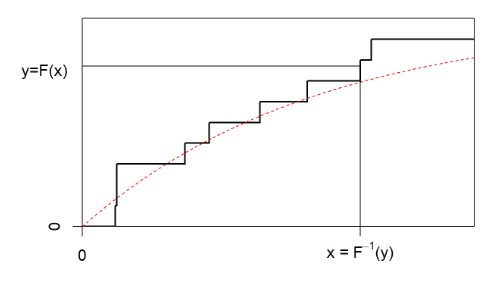
\includegraphics[width=1\linewidth]{images/6.2.1-1} 

}

\end{figure}

Karena \(F_N\) adalah step-function, \(F_n^{-1}\) subtitusi nilai-nilai \(\{x_1,\cdots,x_n\}\) sehingga

\begin{enumerate}
\def\labelenumi{\arabic{enumi}.}
\item
  jika \(y\in(0,1/n)\) (dengan probabilitas \(1 / n\) ) dengan menggambar nilai terkecil ( \(\min\{x_i\}\) )
\item
  jika \(y\in(1/n,2/n)\) (dengan probabilitas \(1 / n\) ) dengan menggambar nilai terkecil kedua,
\end{enumerate}

\ldots{}

\begin{enumerate}
\def\labelenumi{\arabic{enumi}.}
\setcounter{enumi}{2}
\tightlist
\item
  jika \(y\in((n-1)/n,1)\) (dengan probabilitas \(1 / n\) ) kami menggambar nilai terbesar ( \(\max\{x_i\}\) )
\end{enumerate}

\begin{figure}

{\centering 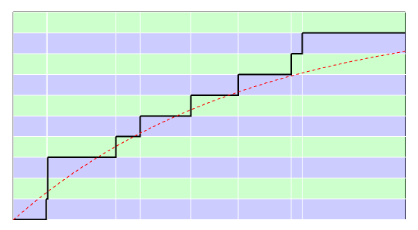
\includegraphics[width=1\linewidth]{images/6.2.1-2} 

}

\end{figure}

Menggunakan metode transformasi terbalik dengan \(F_N\) berarti pengambilan sampel dari \(\{x_1,\cdots,x_n\}\), dengan probabilitas \(1 / n\) . Menghasilkan sampel ukuran bootstrap \(B\) berarti pengambilan sampel dari \(\{x_1,\cdots,x_n\}\) , dengan probabilitas \(1 / n\) , dengan penggantian.

\begin{Shaded}
\begin{Highlighting}[]
\FunctionTok{set.seed}\NormalTok{(}\DecValTok{1}\NormalTok{)}
\NormalTok{n }\OtherTok{\textless{}{-}} \DecValTok{10}
\NormalTok{x }\OtherTok{\textless{}{-}} \FunctionTok{rexp}\NormalTok{(n, }\DecValTok{1}\SpecialCharTok{/}\DecValTok{6}\NormalTok{)}
\NormalTok{m }\OtherTok{\textless{}{-}} \DecValTok{8}
\NormalTok{bootvalues }\OtherTok{\textless{}{-}} \FunctionTok{sample}\NormalTok{(x, }\AttributeTok{size=}\NormalTok{m, }\AttributeTok{replace=}\ConstantTok{TRUE}\NormalTok{)}
\end{Highlighting}
\end{Shaded}

\hypertarget{presisi-bootstrap-bias-standar-deviasi-dan-mean-square-error}{%
\subsection{(6.2.2) Presisi Bootstrap: Bias, Standar Deviasi, dan Mean Square Error}\label{presisi-bootstrap-bias-standar-deviasi-dan-mean-square-error}}

Berikut adalah rangkuman prosedur bootstrap nonparametrik sebagai berikut:

\begin{enumerate}
\def\labelenumi{\arabic{enumi}.}
\item
  Dari sampel \(\{X_1, \ldots, X_n\}\), gambar sampel berukuran n (dengan penggantian), katakanlah, \(X_1^*, \ldots, X_n^*\) . Dari undian yang disimulasikan, hitung statistik minat, dilambangkan sebagai \(\hat{\theta}(X_1^*, \ldots, X_n^*)\) . Panggil ini \(\hat{\theta}_b^*\) untuk ulangan ke-b .
\item
  Ulangi ini \(b=1, \ldots, B\) kali untuk mendapatkan sampel statistik \(\hat{\theta}_1^*, \ldots,\hat{\theta}_B^*\).
\item
  Dari sampel statistik pada Langkah 2,\(\{\hat{\theta}_1^*, \ldots, \hat{\theta}_B^*\}\) hitung ukuran ringkasan minat.
\end{enumerate}

Pada bagian ini, ada tiga langkah ringkasan yaitu bias, standar deviasi, dan mean square error ( MSE ). Tabel dibawah ini merangkum ketiga ukuran. Di Sini, \(\overline{\hat{\theta^*}}\) adalah rata-rata dari \(\{\hat{\theta}_1^*, \ldots,\hat{\theta}_B^*\}\).

\begin{figure}

{\centering 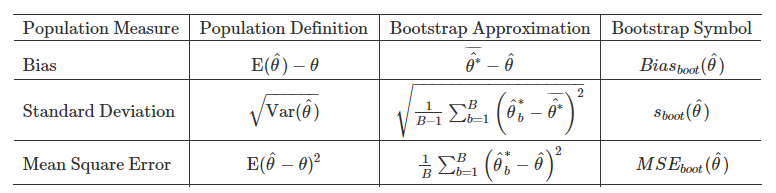
\includegraphics[width=1\linewidth]{images/6.2.1-3} 

}

\end{figure}

\begin{Shaded}
\begin{Highlighting}[]
\CommentTok{\# Example from Derrig et al}
\NormalTok{BIData }\OtherTok{\textless{}{-}} \FunctionTok{read.csv}\NormalTok{(}\StringTok{"Data/DerrigResampling.csv"}\NormalTok{, }\AttributeTok{header =}\NormalTok{T)}
\NormalTok{BIData}\SpecialCharTok{$}\NormalTok{Censored }\OtherTok{\textless{}{-}} \DecValTok{1}\SpecialCharTok{*}\NormalTok{(BIData}\SpecialCharTok{$}\NormalTok{AmountPaid }\SpecialCharTok{\textgreater{}=}\NormalTok{ BIData}\SpecialCharTok{$}\NormalTok{PolicyLimit)}
\NormalTok{BIDataUncensored }\OtherTok{\textless{}{-}} \FunctionTok{subset}\NormalTok{(BIData, Censored }\SpecialCharTok{==} \DecValTok{0}\NormalTok{)}
\NormalTok{LER.boot }\OtherTok{\textless{}{-}} \ControlFlowTok{function}\NormalTok{(ded, data, indices)\{}
\NormalTok{  resample.data }\OtherTok{\textless{}{-}}\NormalTok{ data[indices,]}
\NormalTok{  sumClaims }\OtherTok{\textless{}{-}} \FunctionTok{sum}\NormalTok{(resample.data}\SpecialCharTok{$}\NormalTok{AmountPaid)}
\NormalTok{  sumClaims\_d }\OtherTok{\textless{}{-}} \FunctionTok{sum}\NormalTok{(}\FunctionTok{pmin}\NormalTok{(resample.data}\SpecialCharTok{$}\NormalTok{AmountPaid,ded))}
\NormalTok{  LER }\OtherTok{\textless{}{-}}\NormalTok{   sumClaims\_d}\SpecialCharTok{/}\NormalTok{sumClaims}
  \FunctionTok{return}\NormalTok{(LER)  }
\NormalTok{\}}

\DocumentationTok{\#\#Derrig et al}
\FunctionTok{set.seed}\NormalTok{(}\DecValTok{2019}\NormalTok{)}
\NormalTok{dVec2 }\OtherTok{\textless{}{-}} \FunctionTok{c}\NormalTok{(}\DecValTok{4000}\NormalTok{, }\DecValTok{5000}\NormalTok{, }\DecValTok{10500}\NormalTok{, }\DecValTok{11500}\NormalTok{, }\DecValTok{14000}\NormalTok{, }\DecValTok{18500}\NormalTok{)}
\NormalTok{OutBoot }\OtherTok{\textless{}{-}} \FunctionTok{matrix}\NormalTok{(}\DecValTok{0}\NormalTok{,}\FunctionTok{length}\NormalTok{(dVec2),}\DecValTok{6}\NormalTok{)}
  \ControlFlowTok{for}\NormalTok{ (i }\ControlFlowTok{in} \DecValTok{1}\SpecialCharTok{:}\FunctionTok{length}\NormalTok{(dVec2)) \{}
\NormalTok{OutBoot[i,}\DecValTok{1}\NormalTok{] }\OtherTok{\textless{}{-}}\NormalTok{ dVec2[i]}
\NormalTok{results }\OtherTok{\textless{}{-}} \FunctionTok{boot}\NormalTok{(}\AttributeTok{data=}\NormalTok{BIDataUncensored, }\AttributeTok{statistic=}\NormalTok{LER.boot, }\AttributeTok{R=}\DecValTok{1000}\NormalTok{, }\AttributeTok{ded=}\NormalTok{dVec2[i])}
\NormalTok{OutBoot[i,}\DecValTok{2}\NormalTok{] }\OtherTok{\textless{}{-}}\NormalTok{ results}\SpecialCharTok{$}\NormalTok{t0}
\NormalTok{biasboot }\OtherTok{\textless{}{-}} \FunctionTok{mean}\NormalTok{(results}\SpecialCharTok{$}\NormalTok{t)}\SpecialCharTok{{-}}\NormalTok{results}\SpecialCharTok{$}\NormalTok{t0 }\OtherTok{{-}\textgreater{}}\NormalTok{ OutBoot[i,}\DecValTok{3}\NormalTok{]}
\NormalTok{sdboot }\OtherTok{\textless{}{-}} \FunctionTok{sd}\NormalTok{(results}\SpecialCharTok{$}\NormalTok{t) }\OtherTok{{-}\textgreater{}}\NormalTok{ OutBoot[i,}\DecValTok{4}\NormalTok{]}
\NormalTok{temp }\OtherTok{\textless{}{-}} \FunctionTok{boot.ci}\NormalTok{(results)}
\NormalTok{OutBoot[i,}\DecValTok{5}\NormalTok{] }\OtherTok{\textless{}{-}}\NormalTok{ temp}\SpecialCharTok{$}\NormalTok{normal[}\DecValTok{2}\NormalTok{]}
\NormalTok{OutBoot[i,}\DecValTok{6}\NormalTok{] }\OtherTok{\textless{}{-}}\NormalTok{ temp}\SpecialCharTok{$}\NormalTok{normal[}\DecValTok{3}\NormalTok{]}
\NormalTok{\}}
\end{Highlighting}
\end{Shaded}

\begin{figure}

{\centering 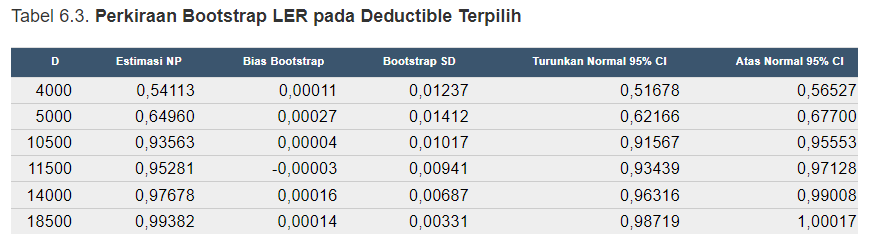
\includegraphics[width=1\linewidth]{images/6.2.1-4} 

}

\end{figure}

Berdasarkan tabel diatas hasil estimasi bootstrap. Misalnya, di D= 14000 , estimasi nonparametrik LER adalah 0,97678. Ini memiliki perkiraan bias 0,00018 dengan standar deviasi 0,00701. Untuk beberapa aplikasi, mungkin ingin menerapkan estimasi bias ke estimasi asli untuk memberikan estimator yang dikoreksi bias. Untuk ilustrasi ini, biasnya kecil sehingga koreksi semacam itu tidak relevan.

Standar deviasi bootstrap memberikan ukuran presisi. Untuk satu penerapan standar deviasi dapat menggunakan pendekatan normal untuk membuat selang kepercayaan. Misalnya, pada \emph{R} fungsi \emph{boot.ci} menghasilkan interval kepercayaan normal sebesar 95\%. Ini dihasilkan dengan membuat interval dua kali panjang standar deviasi bootstrap 1,95994, berpusat di sekitar estimator yang dikoreksi bias (1,95994 adalah kuantil ke-97,5 dari distribusi normal). Misalnya, CI 95\% normal yang lebih rendah di \(D= 14000\) adalah \((0.97678-0.00018)- 1.95994*0.00701\).

\texttt{Contoh\ 6.2.2.} Memperkirakan \(\exp(\mu)\) . Bootstrap dapat digunakan untuk mengukur bias estimator, misalnya. Pertimbangkan di sini sampel \(\mathbf{x}=\{x_1,\cdots,x_n\}\) adalah rata-rata μ .

\begin{Shaded}
\begin{Highlighting}[]
\NormalTok{sample\_x }\OtherTok{\textless{}{-}} \FunctionTok{c}\NormalTok{(}\FloatTok{2.46}\NormalTok{,}\FloatTok{2.80}\NormalTok{,}\FloatTok{3.28}\NormalTok{,}\FloatTok{3.86}\NormalTok{,}\FloatTok{2.85}\NormalTok{,}\FloatTok{3.67}\NormalTok{,}\FloatTok{3.37}\NormalTok{,}\FloatTok{3.40}\NormalTok{,}\FloatTok{5.22}\NormalTok{,}\FloatTok{2.55}\NormalTok{,}
              \FloatTok{2.79}\NormalTok{,}\FloatTok{4.50}\NormalTok{,}\FloatTok{3.37}\NormalTok{,}\FloatTok{2.88}\NormalTok{,}\FloatTok{1.44}\NormalTok{,}\FloatTok{2.56}\NormalTok{,}\FloatTok{2.00}\NormalTok{,}\FloatTok{2.07}\NormalTok{,}\FloatTok{2.19}\NormalTok{,}\FloatTok{1.77}\NormalTok{)}
\end{Highlighting}
\end{Shaded}

Misalkan kuantitas bunga adalah \(\theta=\exp(\mu)\). Penaksir alami akan menjadi \(\widehat{\theta}_1=\exp(\overline{x})\). Estimator ini bias (karena ketidaksetaraan Jensen) tetapi tidak bias secara asimtotik. Untuk sampel, perkiraannya adalah sebagai berikuT

\begin{Shaded}
\begin{Highlighting}[]
\NormalTok{(theta\_1 }\OtherTok{\textless{}{-}} \FunctionTok{exp}\NormalTok{(}\FunctionTok{mean}\NormalTok{(sample\_x)))}
\end{Highlighting}
\end{Shaded}

\begin{verbatim}
## [1] 19.13463
\end{verbatim}

Seseorang dapat menggunakan teorema limit pusat untuk mendapatkan koreksi menggunakan

\[\overline{X}\approx\mathcal{N}\left(\mu,\frac{\sigma^2}{n}\right)\text{ where }\sigma^2=\text{Var}[X_i] ,\]

sehingga dengan fungsi pembangkit momen normal didapatkan

\[\mathrm{E}~\left[\exp(\overline{X})\right] \approx \exp\left(\mu+\frac{\sigma^2}{2n}\right) .\]

Oleh karena itu, seseorang dapat mempertimbangkan secara alami

\[\widehat{\theta}_2=\exp\left(\overline{x}-\frac{\widehat{\sigma}^2}{2n}\right) .\]

\begin{Shaded}
\begin{Highlighting}[]
\NormalTok{n }\OtherTok{\textless{}{-}} \FunctionTok{length}\NormalTok{(sample\_x)}
\NormalTok{(theta\_2 }\OtherTok{\textless{}{-}} \FunctionTok{exp}\NormalTok{(}\FunctionTok{mean}\NormalTok{(sample\_x)}\SpecialCharTok{{-}}\FunctionTok{var}\NormalTok{(sample\_x)}\SpecialCharTok{/}\NormalTok{(}\DecValTok{2}\SpecialCharTok{*}\NormalTok{n)))}
\end{Highlighting}
\end{Shaded}

\begin{verbatim}
## [1] 18.73334
\end{verbatim}

Sebagai strategi lain, seseorang juga dapat menggunakan pendekatan Taylor untuk mendapatkan penaksir yang lebih akurat (seperti dalam metode delta)

\[g(\overline{x})=g(\mu)+(\overline{x}-\mu)g'(\mu)+(\overline{x}-\mu)^2\frac{g''(\mu)}{2}+\cdots\]

Alternatif selanjutnya adalah menggunakan strategi bootstrap dengan sampel bootstrap \(\mathbf{x}^{\ast}_{b}\) sehingga \(\overline{x}^{\ast}_{b}\).

\[\widehat{\theta}_3=\frac{1}{B}\sum_{b=1}^B\exp(\overline{x}^{\ast}_{b}) .\]

\begin{Shaded}
\begin{Highlighting}[]
\FunctionTok{library}\NormalTok{(boot)}
\NormalTok{results }\OtherTok{\textless{}{-}} \FunctionTok{boot}\NormalTok{(}\AttributeTok{data=}\NormalTok{sample\_x, }
                \AttributeTok{statistic=}\ControlFlowTok{function}\NormalTok{(y,indices) }\FunctionTok{exp}\NormalTok{(}\FunctionTok{mean}\NormalTok{(y[indices])), }
                \AttributeTok{R=}\DecValTok{1000}\NormalTok{)}
\NormalTok{theta\_3 }\OtherTok{\textless{}{-}} \FunctionTok{mean}\NormalTok{(results}\SpecialCharTok{$}\NormalTok{t)}
\end{Highlighting}
\end{Shaded}

\begin{figure}

{\centering 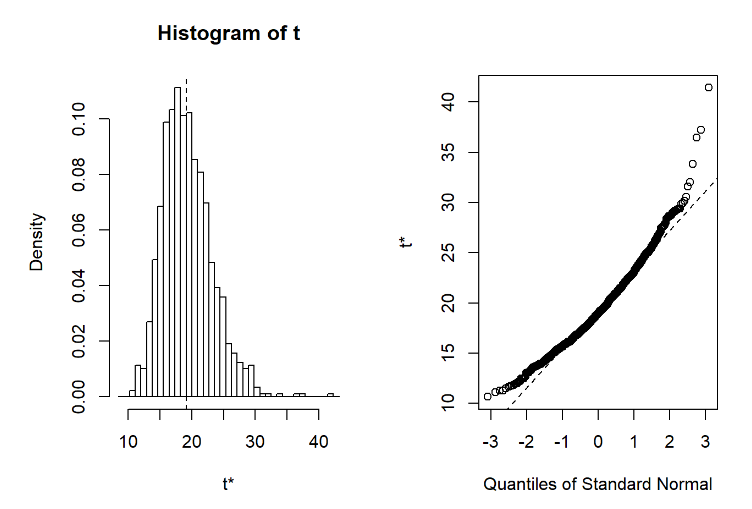
\includegraphics[width=1\linewidth]{images/6.2.2-1} 

}

\end{figure}

\begin{figure}

{\centering 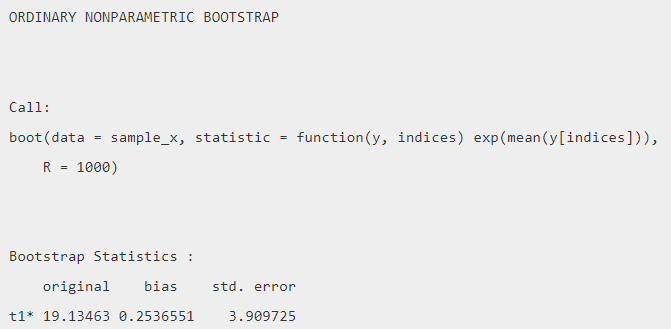
\includegraphics[width=1\linewidth]{images/6.2.2-2} 

}

\end{figure}

Ini menghasilkan tiga estimator, estimator mentah \(\widehat{\theta}_1=19.135\), koreksi urutan kedua \(\widehat{\theta}_2= 18.733\), dan estimator bootstrap \(\widehat{\theta}_3= 19.388\).

Bagaimana cara kerjanya dengan ukuran sampel yang berbeda? Diasumsikan bahwa \(X_i\) dihasilkan dari distribusi lognormal \(LN(0,1)\) , sehingga \(\mu = \exp(0 + 1/2) = 1.648721\) Dan \(\theta = \exp(1.648721)= 5,200326\). Dengan menggunakan simulasi untuk menggambar ukuran sampel.

\begin{Shaded}
\begin{Highlighting}[]
\NormalTok{param }\OtherTok{\textless{}{-}} \ControlFlowTok{function}\NormalTok{(x)\{}
\NormalTok{  n }\OtherTok{\textless{}{-}} \FunctionTok{length}\NormalTok{(x)}
\NormalTok{  theta\_1 }\OtherTok{\textless{}{-}} \FunctionTok{exp}\NormalTok{(}\FunctionTok{mean}\NormalTok{(x))}
\NormalTok{  theta\_2 }\OtherTok{\textless{}{-}} \FunctionTok{exp}\NormalTok{(}\FunctionTok{mean}\NormalTok{(x)}\SpecialCharTok{{-}}\FunctionTok{var}\NormalTok{(x)}\SpecialCharTok{/}\NormalTok{(}\DecValTok{2}\SpecialCharTok{*}\NormalTok{n))}
\NormalTok{  results }\OtherTok{\textless{}{-}} \FunctionTok{boot}\NormalTok{(}\AttributeTok{data=}\NormalTok{x, }
                \AttributeTok{statistic=}\ControlFlowTok{function}\NormalTok{(y,indices) }\FunctionTok{exp}\NormalTok{(}\FunctionTok{mean}\NormalTok{(y[indices])), }
                \AttributeTok{R=}\DecValTok{999}\NormalTok{)}
\NormalTok{  theta\_3 }\OtherTok{\textless{}{-}} \FunctionTok{mean}\NormalTok{(results}\SpecialCharTok{$}\NormalTok{t)}
  \FunctionTok{return}\NormalTok{(}\FunctionTok{c}\NormalTok{(theta\_1,theta\_2,theta\_3))}
\NormalTok{\}}
\FunctionTok{set.seed}\NormalTok{(}\DecValTok{2074}\NormalTok{)}
\NormalTok{ns}\OtherTok{\textless{}{-}} \DecValTok{200}
\NormalTok{est }\OtherTok{\textless{}{-}} \ControlFlowTok{function}\NormalTok{(n)\{}
\NormalTok{call\_param }\OtherTok{\textless{}{-}} \ControlFlowTok{function}\NormalTok{(i) }\FunctionTok{param}\NormalTok{(}\FunctionTok{rlnorm}\NormalTok{(n,}\DecValTok{0}\NormalTok{,}\DecValTok{1}\NormalTok{))}
\NormalTok{V }\OtherTok{\textless{}{-}} \FunctionTok{Vectorize}\NormalTok{(call\_param)(}\DecValTok{1}\SpecialCharTok{:}\NormalTok{ns)}
\FunctionTok{apply}\NormalTok{(V,}\DecValTok{1}\NormalTok{,median)}
\NormalTok{\}}
\NormalTok{VN}\OtherTok{=}\FunctionTok{seq}\NormalTok{(}\DecValTok{15}\NormalTok{,}\DecValTok{100}\NormalTok{,}\AttributeTok{by=}\DecValTok{5}\NormalTok{)}
\NormalTok{Est }\OtherTok{\textless{}{-}} \FunctionTok{Vectorize}\NormalTok{(est)(VN)}
\end{Highlighting}
\end{Shaded}

\begin{Shaded}
\begin{Highlighting}[]
\FunctionTok{matplot}\NormalTok{(VN,}\FunctionTok{t}\NormalTok{(Est),}\AttributeTok{type=}\StringTok{"l"}\NormalTok{, }\AttributeTok{col=}\DecValTok{2}\SpecialCharTok{:}\DecValTok{4}\NormalTok{, }\AttributeTok{lty=}\DecValTok{2}\SpecialCharTok{:}\DecValTok{4}\NormalTok{, }\AttributeTok{ylim=}\FunctionTok{exp}\NormalTok{(}\FunctionTok{exp}\NormalTok{(}\DecValTok{1}\SpecialCharTok{/}\DecValTok{2}\NormalTok{))}\SpecialCharTok{+}\FunctionTok{c}\NormalTok{(}\SpecialCharTok{{-}}\DecValTok{1}\NormalTok{,}\DecValTok{1}\NormalTok{),}
        \AttributeTok{xlab=}\StringTok{"sample size (n)"}\NormalTok{, }\AttributeTok{ylab=}\StringTok{"estimator"}\NormalTok{)}
\FunctionTok{abline}\NormalTok{(}\AttributeTok{h=}\FunctionTok{exp}\NormalTok{(}\FunctionTok{exp}\NormalTok{(}\DecValTok{1}\SpecialCharTok{/}\DecValTok{2}\NormalTok{)),}\AttributeTok{lty=}\DecValTok{1}\NormalTok{, }\AttributeTok{col=}\DecValTok{1}\NormalTok{)}
\FunctionTok{legend}\NormalTok{(}\StringTok{"topleft"}\NormalTok{, }\FunctionTok{c}\NormalTok{(}\StringTok{"raw estimator"}\NormalTok{, }\StringTok{"second order correction"}\NormalTok{, }\StringTok{"bootstrap"}\NormalTok{),}
       \AttributeTok{col=}\DecValTok{2}\SpecialCharTok{:}\DecValTok{4}\NormalTok{,}\AttributeTok{lty=}\DecValTok{2}\SpecialCharTok{:}\DecValTok{4}\NormalTok{, }\AttributeTok{bty=}\StringTok{"n"}\NormalTok{)}
\end{Highlighting}
\end{Shaded}

\begin{figure}

{\centering 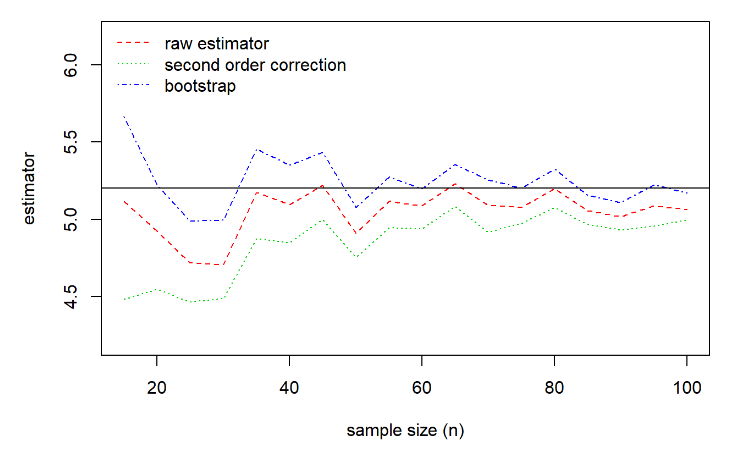
\includegraphics[width=1\linewidth]{images/6.2.2-3} 

}

\end{figure}

Hasil perbandingan dirangkum dalam gambar diatas menunjukkan bahwa estimator bootstrap mendekati nilai parameter sebenarnya untuk hampir semua ukuran sampel. Bias dari ketiga estimator berkurang dengan meningkatnya ukuran sampel.

\hypertarget{interval-keyakinan}{%
\subsection{(6.2.3) Interval Keyakinan}\label{interval-keyakinan}}

Prosedur bootstrap menghasilkan \(B\) bentuk ulang dari \(\hat{\theta}_1^*, \ldots,\hat{\theta}_B^*\) dari penaksir \(\hat{\theta}\) . Dalam Contoh 6.2.1, dapat dilihat bagaimana menggunakan pendekatan normal standar untuk membuat interval kepercayaan untuk parameter yang diinginkan. Namun, mengingat poin utamanya adalah menggunakan bootstrapping untuk menghindari ketergantungan pada asumsi perkiraan normalitas, tidak mengherankan jika tersedia interval kepercayaan alternatif.

Untuk estimator \(\hat{\theta}\) , interval kepercayaan bootstrap dasar adalah

\[\begin{equation} 
  \left(2 \hat{\theta} - q_U, 2 \hat{\theta} - q_L \right) ,
\tag{6.2}
\end{equation}\]

Di mana \(q_L\) Dan \(q_U\) adalah kuantil 2,5\% bawah dan atas dari sampel bootstrap \(\hat{\theta}_1^*, \ldots,\hat{\theta}_B^*\)

Untuk melihat dari mana asalnya, mula-mula \((q_L, q_U)\) menyediakan interval 95\% untuk \(\hat{\theta}_1^*, \ldots,\hat{\theta}_B^*\) . Jadi, untuk acak \(\hat{\theta}_b^*\), ada kemungkinan 95\% itu \(q_L \le \hat{\theta}_b^* \le q_U\). Membalikkan pertidaksamaan dan menjumlahkan \(\hat{\theta}\) ke setiap sisi memberikan interval 95\%

\[\hat{\theta} -q_U \le \hat{\theta} - \hat{\theta}_b^* \le  \hat{\theta} -q_L .\]

Jadi, \(\left( \hat{\theta}-q_U, \hat{\theta} -q_L\right)\) adalah interval 95\% untuk \(\hat{\theta} - \hat{\theta}_b^*\). Ide perkiraan bootstrap mengatakan bahwa ini juga merupakan interval 95\% untuk \(\theta - \hat{\theta}\). Dengan menambahkan \(\hat{\theta}\) ke setiap sisi memberikan interval 95\% dalam persamaan diatas.

Banyak alternatif interval bootstrap yang tersedia. Yang paling mudah dijelaskan adalah interval bootstrap persentil yang didefinisikan sebagai \((q_L,q_U)\).

\texttt{Contoh\ 6.2.3.} Klaim Cidera Tubuh dan Tindakan Risiko. Untuk melihat bagaimana interval kepercayaan bootstrap bekerja, dengan kembali ke klaim otomatis cedera tubuh yang dipertimbangkan dalam Contoh 6.2.1 . Alih-alih rasio eliminasi kerugian, misalkan ingin memperkirakan persentil ke-95 \(F^{-1}(0.95)\) dan ukuran didefinisikan sebagai

\[TVaR_{0.95}[X] = \mathrm{E}[X | X > F^{-1}(0.95)] .\]

Pengukuran ini disebut dengan ekor nilai berisiko; itu adalah nilai yang diharapkan dari X bersyarat X melebihi persentil ke-95. Bagian 10.2 menjelaskan bagaimana quantiles dan tail value-at-risk adalah dua contoh paling penting dari apa yang disebut sebagai ukuran risiko . Untuk saat ini, hanya akan menganggap ini sebagai ukuran yang ingin diperkirakan. Untuk persentil, dengan menggunakan estimator nonparametrik \(F^{-1}_n(0.95)\) didefinisikan dalam Bagian 4.1.1.3 . Untuk tail value-at-risk, menggunakan prinsip plug-in untuk menentukan estimator nonparametrik

\[TVaR_{n,0.95}[X] = \frac{\sum_{i=1}^n X_i I(X_i > F^{-1}_n(0.95))}{\sum_{i=1}^n I(X_i > F^{-1}_n(0.95))} ~.\]

Dalam ungkapan ini, penyebut menghitung jumlah pengamatan yang melebihi persentil ke-95 \(F^{-1}_n(0.95)\) . Pembilang menjumlahkan kerugian untuk pengamatan yang melebihi \(F^{-1}_n(0.95)\) . Tabel dibawah ini merangkum penaksir untuk pecahan terpilih.

\begin{Shaded}
\begin{Highlighting}[]
\CommentTok{\# Example from Derrig et al}
\CommentTok{\#BIData \textless{}{-} read.csv("Data/DerrigResampling.csv", header =T)}
\NormalTok{BIData}\SpecialCharTok{$}\NormalTok{Censored }\OtherTok{\textless{}{-}} \DecValTok{1}\SpecialCharTok{*}\NormalTok{(BIData}\SpecialCharTok{$}\NormalTok{AmountPaid }\SpecialCharTok{\textgreater{}=}\NormalTok{ BIData}\SpecialCharTok{$}\NormalTok{PolicyLimit)}
\NormalTok{BIDataUncensored }\OtherTok{\textless{}{-}} \FunctionTok{subset}\NormalTok{(BIData, Censored }\SpecialCharTok{==} \DecValTok{0}\NormalTok{)}

\FunctionTok{set.seed}\NormalTok{(}\DecValTok{2017}\NormalTok{)}
\NormalTok{PercentVec }\OtherTok{\textless{}{-}} \FunctionTok{c}\NormalTok{(}\FloatTok{0.50}\NormalTok{, }\FloatTok{0.80}\NormalTok{, }\FloatTok{0.90}\NormalTok{, }\FloatTok{0.95}\NormalTok{, }\FloatTok{0.98}\NormalTok{)}
\NormalTok{OutBoot1 }\OtherTok{\textless{}{-}} \FunctionTok{matrix}\NormalTok{(}\DecValTok{0}\NormalTok{,}\DecValTok{5}\NormalTok{,}\DecValTok{10}\NormalTok{)}
\ControlFlowTok{for}\NormalTok{ (i }\ControlFlowTok{in} \DecValTok{1}\SpecialCharTok{:}\FunctionTok{length}\NormalTok{(PercentVec)) \{}
\NormalTok{OutBoot1[i,}\DecValTok{1}\NormalTok{] }\OtherTok{\textless{}{-}}\NormalTok{ PercentVec[i]}
\NormalTok{results }\OtherTok{\textless{}{-}} \FunctionTok{boot}\NormalTok{(}\AttributeTok{data=}\NormalTok{BIDataUncensored}\SpecialCharTok{$}\NormalTok{AmountPaid,}
                \AttributeTok{statistic=}\ControlFlowTok{function}\NormalTok{(X,indices)}
                    \FunctionTok{quantile}\NormalTok{(X[indices],PercentVec[i]),}
                 \AttributeTok{R=}\DecValTok{1000}\NormalTok{)}
\ControlFlowTok{if}\NormalTok{ (i}\SpecialCharTok{==}\DecValTok{1}\NormalTok{)\{bootreal }\OtherTok{\textless{}{-}}\NormalTok{ results}\SpecialCharTok{$}\NormalTok{t\}}
\NormalTok{OutBoot1[i,}\DecValTok{2}\NormalTok{] }\OtherTok{\textless{}{-}}\NormalTok{ results}\SpecialCharTok{$}\NormalTok{t0}
\NormalTok{OutBoot1[i,}\DecValTok{3}\NormalTok{] }\OtherTok{\textless{}{-}} \FunctionTok{mean}\NormalTok{(results}\SpecialCharTok{$}\NormalTok{t)}\SpecialCharTok{{-}}\NormalTok{results}\SpecialCharTok{$}\NormalTok{t0 }
\NormalTok{OutBoot1[i,}\DecValTok{4}\NormalTok{] }\OtherTok{\textless{}{-}} \FunctionTok{sd}\NormalTok{(results}\SpecialCharTok{$}\NormalTok{t) }
\NormalTok{temp }\OtherTok{\textless{}{-}} \FunctionTok{boot.ci}\NormalTok{(results, }\AttributeTok{type =} \FunctionTok{c}\NormalTok{(}\StringTok{"norm"}\NormalTok{, }\StringTok{"basic"}\NormalTok{, }\StringTok{"perc"}\NormalTok{))}
\NormalTok{OutBoot1[i,}\DecValTok{5}\NormalTok{] }\OtherTok{\textless{}{-}}\NormalTok{ temp}\SpecialCharTok{$}\NormalTok{normal[}\DecValTok{2}\NormalTok{]}
\NormalTok{OutBoot1[i,}\DecValTok{6}\NormalTok{] }\OtherTok{\textless{}{-}}\NormalTok{ temp}\SpecialCharTok{$}\NormalTok{normal[}\DecValTok{3}\NormalTok{]}
\NormalTok{OutBoot1[i,}\DecValTok{7}\NormalTok{] }\OtherTok{\textless{}{-}}\NormalTok{ temp}\SpecialCharTok{$}\NormalTok{basic[}\DecValTok{4}\NormalTok{]}
\NormalTok{OutBoot1[i,}\DecValTok{8}\NormalTok{] }\OtherTok{\textless{}{-}}\NormalTok{ temp}\SpecialCharTok{$}\NormalTok{basic[}\DecValTok{5}\NormalTok{]}
\NormalTok{OutBoot1[i,}\DecValTok{9}\NormalTok{] }\OtherTok{\textless{}{-}}\NormalTok{ temp}\SpecialCharTok{$}\NormalTok{percent[}\DecValTok{4}\NormalTok{]}
\NormalTok{OutBoot1[i,}\DecValTok{10}\NormalTok{] }\OtherTok{\textless{}{-}}\NormalTok{ temp}\SpecialCharTok{$}\NormalTok{percent[}\DecValTok{5}\NormalTok{]}
\NormalTok{\}}
\end{Highlighting}
\end{Shaded}

\begin{figure}

{\centering 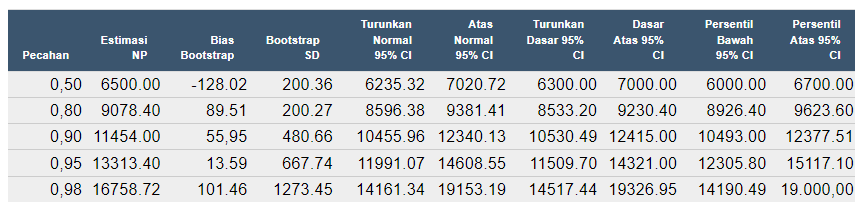
\includegraphics[width=1\linewidth]{images/6.2.3-1} 

}

\end{figure}

Misalnya, ketika pecahannya adalah 0,50, dapat melihat bahwa kuantil 2,5 bawah dan atas dari simulasi bootstrap adalah \(q_L= 6000\) dan \(q_U= 6700\). Ini membentuk interval kepercayaan bootstrap persentil. Dengan estimator nonparametrik \(6500\), ini menghasilkan batas bawah dan atas interval kepercayaan dasar masing-masing \(6300\) dan \(7000\).

\begin{Shaded}
\begin{Highlighting}[]
\NormalTok{CTE.boot }\OtherTok{\textless{}{-}} \ControlFlowTok{function}\NormalTok{(data, indices, RiskLevel)\{}
\NormalTok{  resample.data }\OtherTok{\textless{}{-}}\NormalTok{ data[indices,]}
\NormalTok{  X }\OtherTok{\textless{}{-}}\NormalTok{ resample.data}\SpecialCharTok{$}\NormalTok{AmountPaid}
\NormalTok{  cutoff }\OtherTok{\textless{}{-}} \FunctionTok{quantile}\NormalTok{(X, RiskLevel)}
\NormalTok{  CTE }\OtherTok{\textless{}{-}} \FunctionTok{sum}\NormalTok{(X}\SpecialCharTok{*}\NormalTok{(X }\SpecialCharTok{\textgreater{}}\NormalTok{ cutoff))}\SpecialCharTok{/}\FunctionTok{sum}\NormalTok{(X }\SpecialCharTok{\textgreater{}}\NormalTok{ cutoff)}
  \FunctionTok{return}\NormalTok{(CTE) }
\NormalTok{\}}

\FunctionTok{set.seed}\NormalTok{(}\DecValTok{2017}\NormalTok{)  }
\NormalTok{PercentVec }\OtherTok{\textless{}{-}} \FunctionTok{c}\NormalTok{(}\FloatTok{0.50}\NormalTok{, }\FloatTok{0.80}\NormalTok{, }\FloatTok{0.90}\NormalTok{, }\FloatTok{0.95}\NormalTok{, }\FloatTok{0.98}\NormalTok{)}
\NormalTok{OutBoot1 }\OtherTok{\textless{}{-}} \FunctionTok{matrix}\NormalTok{(}\DecValTok{0}\NormalTok{,}\DecValTok{5}\NormalTok{,}\DecValTok{10}\NormalTok{)}
  \ControlFlowTok{for}\NormalTok{ (i }\ControlFlowTok{in} \DecValTok{1}\SpecialCharTok{:}\FunctionTok{length}\NormalTok{(PercentVec)) \{}
\NormalTok{OutBoot1[i,}\DecValTok{1}\NormalTok{] }\OtherTok{\textless{}{-}}\NormalTok{ PercentVec[i]}
\NormalTok{results }\OtherTok{\textless{}{-}} \FunctionTok{boot}\NormalTok{(}\AttributeTok{data=}\NormalTok{BIDataUncensored, }\AttributeTok{statistic=}\NormalTok{CTE.boot, }\AttributeTok{R=}\DecValTok{1000}\NormalTok{, }\AttributeTok{RiskLevel=}\NormalTok{PercentVec[i])}
\NormalTok{OutBoot1[i,}\DecValTok{2}\NormalTok{] }\OtherTok{\textless{}{-}}\NormalTok{ results}\SpecialCharTok{$}\NormalTok{t0}
\NormalTok{OutBoot1[i,}\DecValTok{3}\NormalTok{] }\OtherTok{\textless{}{-}} \FunctionTok{mean}\NormalTok{(results}\SpecialCharTok{$}\NormalTok{t)}\SpecialCharTok{{-}}\NormalTok{results}\SpecialCharTok{$}\NormalTok{t0 }
\NormalTok{OutBoot1[i,}\DecValTok{4}\NormalTok{] }\OtherTok{\textless{}{-}} \FunctionTok{sd}\NormalTok{(results}\SpecialCharTok{$}\NormalTok{t) }
\NormalTok{temp }\OtherTok{\textless{}{-}} \FunctionTok{boot.ci}\NormalTok{(results, }\AttributeTok{type =} \FunctionTok{c}\NormalTok{(}\StringTok{"norm"}\NormalTok{, }\StringTok{"basic"}\NormalTok{, }\StringTok{"perc"}\NormalTok{))}
\NormalTok{OutBoot1[i,}\DecValTok{5}\NormalTok{] }\OtherTok{\textless{}{-}}\NormalTok{ temp}\SpecialCharTok{$}\NormalTok{normal[}\DecValTok{2}\NormalTok{]}
\NormalTok{OutBoot1[i,}\DecValTok{6}\NormalTok{] }\OtherTok{\textless{}{-}}\NormalTok{ temp}\SpecialCharTok{$}\NormalTok{normal[}\DecValTok{3}\NormalTok{]}
\NormalTok{OutBoot1[i,}\DecValTok{7}\NormalTok{] }\OtherTok{\textless{}{-}}\NormalTok{ temp}\SpecialCharTok{$}\NormalTok{basic[}\DecValTok{4}\NormalTok{]}
\NormalTok{OutBoot1[i,}\DecValTok{8}\NormalTok{] }\OtherTok{\textless{}{-}}\NormalTok{ temp}\SpecialCharTok{$}\NormalTok{basic[}\DecValTok{5}\NormalTok{]}
\NormalTok{OutBoot1[i,}\DecValTok{9}\NormalTok{] }\OtherTok{\textless{}{-}}\NormalTok{ temp}\SpecialCharTok{$}\NormalTok{percent[}\DecValTok{4}\NormalTok{]}
\NormalTok{OutBoot1[i,}\DecValTok{10}\NormalTok{] }\OtherTok{\textless{}{-}}\NormalTok{ temp}\SpecialCharTok{$}\NormalTok{percent[}\DecValTok{5}\NormalTok{]}
\NormalTok{  \}}
\end{Highlighting}
\end{Shaded}

\begin{figure}

{\centering 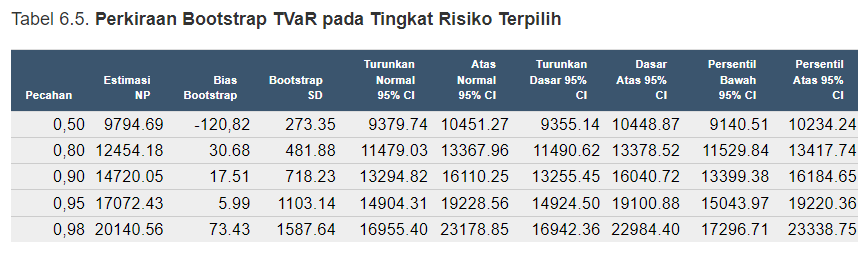
\includegraphics[width=1\linewidth]{images/6.2.3-2} 

}

\end{figure}

Tabel di atas menunjukkan kalkulasi serupa untuk tail value-at-risk. Dalam setiap kasus, dapat melihat bahwa deviasi standar bootstrap meningkat seiring dengan peningkatan fraksi. Hal ini karena ada lebih sedikit pengamatan untuk memperkirakan kuantil seiring meningkatnya fraksi, yang menyebabkan ketidaktepatan yang lebih besar. Interval kepercayaan juga menjadi lebih lebar. Menariknya, tampaknya tidak ada pola yang sama dalam estimasi bias tersebut.

\hypertarget{bootstrap-parametrik}{%
\subsection{(6.2.4) Bootstrap Parametrik}\label{bootstrap-parametrik}}

Gagasan dari bootstrap nonparametrik adalah untuk mengambil sampel ulang dengan menggambar variabel independen dari fungsi distribusi kumulatif empiris \(F_n\). Sebaliknya, dengan bootstrap parametrik, kami menarik variabel independen dari \(F_{\widehat{\theta}}\) di mana distribusi yang mendasarinya diasumsikan dalam keluarga parametrik \(\mathcal{F}=\{F_{\theta},\theta\in\Theta\}\) . Biasanya, parameter dari distribusi ini diperkirakan berdasarkan sampel dan dinotasikan sebagai \(\hat{\theta}\).

\texttt{contoh\ 6.2.4.} distribusi lognormal. Pertimbangkan lagi kumpulan datanya

\begin{Shaded}
\begin{Highlighting}[]
\NormalTok{sample\_x }\OtherTok{\textless{}{-}} \FunctionTok{c}\NormalTok{(}\FloatTok{2.46}\NormalTok{,}\FloatTok{2.80}\NormalTok{,}\FloatTok{3.28}\NormalTok{,}\FloatTok{3.86}\NormalTok{,}\FloatTok{2.85}\NormalTok{,}\FloatTok{3.67}\NormalTok{,}\FloatTok{3.37}\NormalTok{,}\FloatTok{3.40}\NormalTok{,}
              \FloatTok{5.22}\NormalTok{,}\FloatTok{2.55}\NormalTok{,}\FloatTok{2.79}\NormalTok{,}\FloatTok{4.50}\NormalTok{,}\FloatTok{3.37}\NormalTok{,}\FloatTok{2.88}\NormalTok{,}\FloatTok{1.44}\NormalTok{,}\FloatTok{2.56}\NormalTok{,}\FloatTok{2.00}\NormalTok{,}\FloatTok{2.07}\NormalTok{,}\FloatTok{2.19}\NormalTok{,}\FloatTok{1.77}\NormalTok{)}
\end{Highlighting}
\end{Shaded}

Bootstrap klasik (nonparametrik) didasarkan pada contoh berikut.

\begin{Shaded}
\begin{Highlighting}[]
\NormalTok{x }\OtherTok{\textless{}{-}} \FunctionTok{sample}\NormalTok{(sample\_x,}\AttributeTok{replace=}\ConstantTok{TRUE}\NormalTok{)}
\end{Highlighting}
\end{Shaded}

Sebagai gantinya, untuk bootstrap parametrik harus mengasumsikan bahwa distribusi dari \(x_i\) adalah dari kelompok tertentu. Sebagai contoh, kode berikut menggunakan distribusi lognormal.

\begin{Shaded}
\begin{Highlighting}[]
\FunctionTok{library}\NormalTok{(MASS)}
\NormalTok{fit }\OtherTok{\textless{}{-}} \FunctionTok{fitdistr}\NormalTok{(sample\_x, dlnorm, }\FunctionTok{list}\NormalTok{(}\AttributeTok{meanlog =} \DecValTok{1}\NormalTok{, }\AttributeTok{sdlog =} \DecValTok{1}\NormalTok{))}
\NormalTok{fit}
\end{Highlighting}
\end{Shaded}

\begin{figure}

{\centering 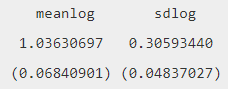
\includegraphics[width=1\linewidth]{images/6.2.4-1} 

}

\end{figure}

\begin{Shaded}
\begin{Highlighting}[]
\NormalTok{x }\OtherTok{\textless{}{-}} \FunctionTok{rlnorm}\NormalTok{(}\FunctionTok{length}\NormalTok{(sample\_x), }\AttributeTok{meanlog=}\NormalTok{fit}\SpecialCharTok{$}\NormalTok{estimate[}\DecValTok{1}\NormalTok{], }\AttributeTok{sdlog=}\NormalTok{fit}\SpecialCharTok{$}\NormalTok{estimate[}\DecValTok{2}\NormalTok{])}
\end{Highlighting}
\end{Shaded}

\begin{Shaded}
\begin{Highlighting}[]
\FunctionTok{set.seed}\NormalTok{(}\DecValTok{2074}\NormalTok{)}
\NormalTok{CV }\OtherTok{\textless{}{-}} \FunctionTok{matrix}\NormalTok{(}\ConstantTok{NA}\NormalTok{,}\FloatTok{1e5}\NormalTok{,}\DecValTok{2}\NormalTok{)}
\ControlFlowTok{for}\NormalTok{(s }\ControlFlowTok{in} \DecValTok{1}\SpecialCharTok{:}\FunctionTok{nrow}\NormalTok{(CV))\{}
\NormalTok{x1 }\OtherTok{\textless{}{-}} \FunctionTok{sample}\NormalTok{(sample\_x,}\AttributeTok{replace=}\ConstantTok{TRUE}\NormalTok{)}
\NormalTok{x2 }\OtherTok{\textless{}{-}} \FunctionTok{rlnorm}\NormalTok{(}\FunctionTok{length}\NormalTok{(sample\_x), }\AttributeTok{meanlog=}\NormalTok{fit}\SpecialCharTok{$}\NormalTok{estimate[}\DecValTok{1}\NormalTok{], }\AttributeTok{sdlog=}\NormalTok{fit}\SpecialCharTok{$}\NormalTok{estimate[}\DecValTok{2}\NormalTok{])}
\NormalTok{CV[s,] }\OtherTok{\textless{}{-}} \FunctionTok{c}\NormalTok{(}\FunctionTok{sd}\NormalTok{(x1)}\SpecialCharTok{/}\FunctionTok{mean}\NormalTok{(x1),}\FunctionTok{sd}\NormalTok{(x2)}\SpecialCharTok{/}\FunctionTok{mean}\NormalTok{(x2))}
\NormalTok{\}}
\end{Highlighting}
\end{Shaded}

\begin{Shaded}
\begin{Highlighting}[]
\FunctionTok{plot}\NormalTok{(}\FunctionTok{density}\NormalTok{(CV[,}\DecValTok{1}\NormalTok{]),}\AttributeTok{col=}\StringTok{"red"}\NormalTok{,}\AttributeTok{main=}\StringTok{""}\NormalTok{,}\AttributeTok{xlab=}\StringTok{"Coefficient of Variation"}\NormalTok{, }\AttributeTok{lty=}\DecValTok{1}\NormalTok{)}
\FunctionTok{lines}\NormalTok{(}\FunctionTok{density}\NormalTok{(CV[,}\DecValTok{2}\NormalTok{]),}\AttributeTok{col=}\StringTok{"blue"}\NormalTok{,}\AttributeTok{lty=}\DecValTok{2}\NormalTok{)}
\FunctionTok{abline}\NormalTok{(}\AttributeTok{v=}\FunctionTok{sd}\NormalTok{(sample\_x)}\SpecialCharTok{/}\FunctionTok{mean}\NormalTok{(sample\_x),}\AttributeTok{lty=}\DecValTok{3}\NormalTok{)}
\FunctionTok{legend}\NormalTok{(}\StringTok{"topright"}\NormalTok{,}\FunctionTok{c}\NormalTok{(}\StringTok{"nonparametric"}\NormalTok{,}\StringTok{"parametric(LN)"}\NormalTok{),}
       \AttributeTok{col=}\FunctionTok{c}\NormalTok{(}\StringTok{"red"}\NormalTok{,}\StringTok{"blue"}\NormalTok{),}\AttributeTok{lty=}\DecValTok{1}\SpecialCharTok{:}\DecValTok{2}\NormalTok{,}\AttributeTok{bty=}\StringTok{"n"}
\end{Highlighting}
\end{Shaded}

\begin{figure}

{\centering 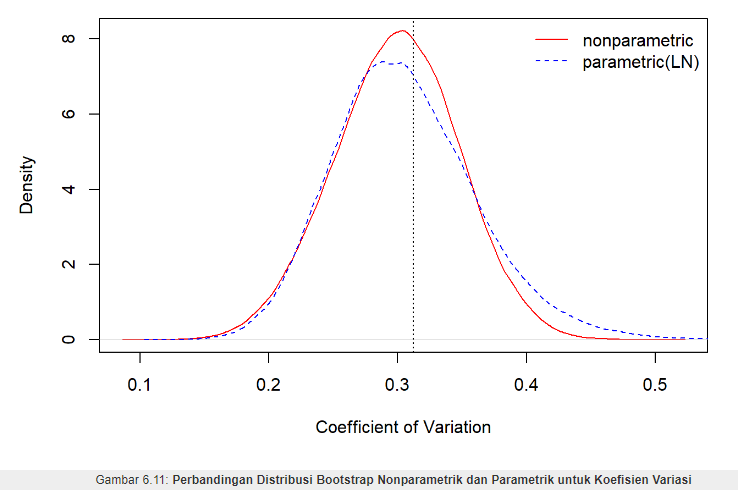
\includegraphics[width=1\linewidth]{images/6.2.3-3} 

}

\end{figure}

Grafik di atas membandingkan distribusi bootstrap untuk koefisien variasi, yang satu berdasarkan pendekatan nonparametrik dan yang lainnya berdasarkan pendekatan parametrik, dengan asumsi distribusi lognormal.

\texttt{Contoh\ 6.2.5.} Pengamatan yang Disensor Bootstrap.

Bootstrap parametrik menarik realisasi simulasi dari perkiraan parametrik dari fungsi distribusi. Dengan cara yang sama, sehingga dapat menggambar realisasi simulasi dari estimasi fungsi distribusi. Sebagai salah satu contoh, dengan mengambil dari estimasi yang dihaluskan dari fungsi distribusi yang diperkenalkan di Bagian 4.1.1.4 . Kasus khusus lainnya, yang dipertimbangkan di sini adalah menggambar estimasi dari estimator Kaplan-Meier yang dibahas di Bagian 4.3.2.2. Dengan cara ini, dapat ditangani pengamatan yang disensor.

Secara khusus, kembali ke data cedera tubuh pada Contoh 6.2.1 dan 6.2.3 tetapi sekarang menyertakan 17 klaim yang disensor oleh batasan kebijakan. Dalam Contoh 4.3.6 menggunakan kumpulan data lengkap ini untuk mengestimasi estimator Kaplan-Meier dari fungsi survival yang diperkenalkan di Bagian 4.3.2.2 . Tabel 6.6 menyajikan estimasi bootstrap kuantil dari estimator fungsi survival Kaplan-Meier. Ini termasuk perkiraan presisi bootstrap, bias dan standar deviasi, serta interval kepercayaan dasar 95\%.

\begin{Shaded}
\begin{Highlighting}[]
\CommentTok{\# Example from Derrig et al}
\FunctionTok{library}\NormalTok{(survival)                }\CommentTok{\# for Surv(), survfit()}
\NormalTok{BIData}\SpecialCharTok{$}\NormalTok{UnCensored }\OtherTok{\textless{}{-}} \DecValTok{1}\SpecialCharTok{*}\NormalTok{(BIData}\SpecialCharTok{$}\NormalTok{AmountPaid }\SpecialCharTok{\textless{}}\NormalTok{ BIData}\SpecialCharTok{$}\NormalTok{PolicyLimit)}
\DocumentationTok{\#\# KM estimate}
\NormalTok{KM0 }\OtherTok{\textless{}{-}} \FunctionTok{survfit}\NormalTok{(}\FunctionTok{Surv}\NormalTok{(AmountPaid, UnCensored) }\SpecialCharTok{\textasciitilde{}} \DecValTok{1}\NormalTok{,  }
               \AttributeTok{type=}\StringTok{"kaplan{-}meier"}\NormalTok{, }\AttributeTok{data=}\NormalTok{BIData)}

\FunctionTok{set.seed}\NormalTok{(}\DecValTok{2019}\NormalTok{)}
\NormalTok{PercentVec }\OtherTok{\textless{}{-}} \FunctionTok{c}\NormalTok{(}\FloatTok{0.50}\NormalTok{, }\FloatTok{0.80}\NormalTok{, }\FloatTok{0.90}\NormalTok{, }\FloatTok{0.95}\NormalTok{, }\FloatTok{0.98}\NormalTok{)}
\NormalTok{OutBoot1 }\OtherTok{\textless{}{-}} \FunctionTok{matrix}\NormalTok{(}\ConstantTok{NA}\NormalTok{,}\DecValTok{5}\NormalTok{,}\DecValTok{6}\NormalTok{)}
\NormalTok{KM.survobj }\OtherTok{\textless{}{-}} \FunctionTok{Surv}\NormalTok{(BIData}\SpecialCharTok{$}\NormalTok{AmountPaid, BIData}\SpecialCharTok{$}\NormalTok{UnCensored) }
\ControlFlowTok{for}\NormalTok{ (i }\ControlFlowTok{in} \DecValTok{1}\SpecialCharTok{:}\FunctionTok{length}\NormalTok{(PercentVec)) \{}
\NormalTok{OutBoot1[i,}\DecValTok{1}\NormalTok{] }\OtherTok{\textless{}{-}}\NormalTok{ PercentVec[i]}
\NormalTok{results }\OtherTok{\textless{}{-}} \FunctionTok{bootkm}\NormalTok{(KM.survobj, }\AttributeTok{q=}\DecValTok{1}\SpecialCharTok{{-}}\NormalTok{PercentVec[i], }\AttributeTok{B=}\DecValTok{1000}\NormalTok{, }\AttributeTok{pr =} \ConstantTok{FALSE}\NormalTok{)}
\ControlFlowTok{if}\NormalTok{ (i}\SpecialCharTok{==}\DecValTok{1}\NormalTok{)\{bootreal }\OtherTok{\textless{}{-}}\NormalTok{ results\}}
\NormalTok{OutBoot1[i,}\DecValTok{2}\NormalTok{] }\OtherTok{\textless{}{-}} \FunctionTok{quantile}\NormalTok{(KM0, PercentVec[i])}\SpecialCharTok{$}\NormalTok{quantile}
\NormalTok{OutBoot1[i,}\DecValTok{3}\NormalTok{] }\OtherTok{\textless{}{-}} \FunctionTok{mean}\NormalTok{(results)}\SpecialCharTok{{-}}\NormalTok{OutBoot1[i,}\DecValTok{2}\NormalTok{]}
\NormalTok{OutBoot1[i,}\DecValTok{4}\NormalTok{] }\OtherTok{\textless{}{-}} \FunctionTok{sd}\NormalTok{(results) }
\CommentTok{\# temp \textless{}{-} boot.ci(results, type = c("norm",  "basic","perc"))}
\NormalTok{OutBoot1[i,}\DecValTok{5}\NormalTok{] }\OtherTok{\textless{}{-}} \DecValTok{2}\SpecialCharTok{*}\NormalTok{OutBoot1[i,}\DecValTok{2}\NormalTok{]}\SpecialCharTok{{-}}\FunctionTok{quantile}\NormalTok{(results,.}\DecValTok{975}\NormalTok{, }\AttributeTok{type=}\DecValTok{6}\NormalTok{)}
\NormalTok{OutBoot1[i,}\DecValTok{6}\NormalTok{] }\OtherTok{\textless{}{-}} \DecValTok{2}\SpecialCharTok{*}\NormalTok{OutBoot1[i,}\DecValTok{2}\NormalTok{]}\SpecialCharTok{{-}}\FunctionTok{quantile}\NormalTok{(results,.}\DecValTok{025}\NormalTok{, }\AttributeTok{type=}\DecValTok{6}\NormalTok{)}
\NormalTok{\}}
\end{Highlighting}
\end{Shaded}

\begin{figure}

{\centering 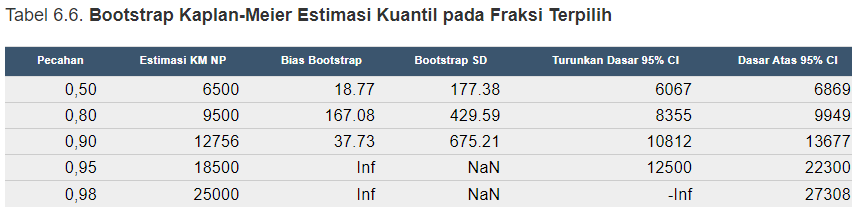
\includegraphics[width=1\linewidth]{images/6.2.3-4} 

}

\end{figure}

Hasil pada tabel di atas konsisten dengan hasil untuk subsampel tanpa sensor pada Tabel 6.4 . Pada tabel di atas tercatat kesulitan dalam memperkirakan kuantil pada pecahan besar karena penyensoran. Namun, untuk fraksi berukuran sedang (0,50, 0,80, dan 0,90), estimasi nonparametrik Kaplan-Meier (KM NP) dari kuantil konsisten dengan Tabel 6.4 . Standar Deviasi bootstrap lebih kecil pada 0,50 (sesuai dengan median) tetapi lebih besar pada level 0,80 dan 0,90. Analisis data tersensor yang dirangkum dalam tabel di atas menggunakan lebih banyak data daripada analisis subsampel tanpa sensor pada Tabel 6.4 , tetapi juga mengalami kesulitan dalam mengekstraksi informasi untuk kuantil besar.
=======
>>>>>>> f9a746c5b24126443ff5b71c4335db228507f5bc
\hypertarget{simulation-and-resampling}{%
\chapter{Simulation and Resampling}\label{simulation-and-resampling}}
>>>>>>> 1507448987ea466b9753eba8674625da5f907a7f

\hypertarget{premium-foundations}{%
\chapter{Premium Foundations}\label{premium-foundations}}

\hypertarget{pengenalan-ratemaking}{%
\chapter{7.1 Pengenalan Ratemaking}\label{pengenalan-ratemaking}}

Pada bagian ini, Anda akan belajar cara:

Menggambarkan ekspektasi sebagai metode dasar untuk menentukan premi asuransi
Menganalisis persamaan akuntansi untuk menghubungkan premi dengan kerugian, biaya, dan keuntungan
Merangkum strategi untuk memperluas penetapan harga untuk mencakup risiko heterogen dan tren dari waktu ke waktu.

Bab ini menjelaskan bagaimana menentukan harga yang tepat untuk produk asuransi, yang dikenal sebagai premi. Premi adalah jumlah uang yang dibebankan untuk perlindungan asuransi terhadap kejadian yang tidak pasti. Dalam asuransi, harga/premi ini dikenal sebagai tarif karena dinyatakan dalam unit standar, misalnya harga per seribu dolar pertanggungan atas rumah atau manfaat jika terjadi kematian.

Namun, keunikan asuransi adalah bahwa biaya perlindungan asuransi tidak diketahui pada saat penjualan kontrak. Biaya mungkin tidak terungkap selama berbulan-bulan atau bertahun-tahun, tergantung pada kejadian yang diasuransikan. Oleh karena itu, penetapan harga asuransi berbeda dengan pendekatan ekonomi pada umumnya.

Dalam pendekatan penetapan harga aktuaria tradisional, harga ditentukan sebagai fungsi dari biaya asuransi. Premi dianggap sebagai sumber pendapatan yang menyediakan pembayaran klaim, biaya kontrak, dan margin operasi, yang dapat dirumuskan dalam persamaan akuntansi:

\begin{equation}
\small{
\text{Premium = Loss + Expense + UW Profit} .
}
\end{equation}

Namun, ada pasar asuransi di mana harga aktuaria hanya memberikan masukan untuk harga pasar umum. Untuk memperkuat perbedaan ini, premi berbasis biaya aktuaria kadang-kadang dikenal sebagai harga teknis. Oleh karena itu, keputusan perusahaan seperti penetapan harga harus dievaluasi dengan mengacu pada dampaknya terhadap nilai pasar perusahaan. Tujuan ini lebih komprehensif daripada gagasan statis tentang maksimalisasi laba.

Istilah Biaya dapat dibagi menjadi biaya yang bervariasi berdasarkan premi, seperti komisi penjualan, dan yang tidak, seperti biaya bangunan dan gaji karyawan. Istilah Keuntungan UW adalah singkatan dari keuntungan underwriting dan dapat mencakup biaya modal. Persamaan ini berlaku untuk jumlah banyak kontrak, atau portofolio, dan digunakan untuk membantu menetapkan premi, seperti dengan menetapkan tujuan laba.

Istilah kerugian dalam persamaan tersebut didasarkan pada biaya yang diharapkan, karena sulit untuk memprediksi kerugian yang tepat untuk masing-masing kontrak. Namun, teks tersebut mengakui bahwa pendekatan ini mengasumsikan adanya ketidakpastian dan memperkenalkan prinsip-prinsip premi alternatif yang memasukkan ketidakpastian ke dalam penetapan harga. Bab ini juga memperluas pertimbangan penetapan harga ke kumpulan risiko yang heterogen dan membahas perkembangan dan tren pengalaman kerugian untuk mengembangkan tingkat suku bunga ke depan.

Terakhir, bab ini memperkenalkan metode untuk memilih premi dengan membandingkan metode pemeringkatan premi dengan kerugian dari portofolio yang ditahan dan memilih metode yang menghasilkan kecocokan terbaik dengan data yang ditahan. Bab ini juga mencakup suplemen teknis mengenai peraturan pemerintah tentang tarif asuransi.

\hypertarget{metode-penentuan-tarif-gabungan}{%
\chapter{7.2 Metode Penentuan Tarif Gabungan}\label{metode-penentuan-tarif-gabungan}}

Pada bagian ini, Anda akan belajar tentang:

\begin{itemize}
\tightlist
\item
  Definisi pure premium sebagai biaya kerugian serta dalam hal frekuensi dan keparahan.
\item
  Menghitung tarif yang diindikasikan menggunakan pure premiums, biaya, dan beban keuntungan.
\item
  Definisi rasio kerugian.
\item
  Menghitung perubahan tarif yang diindikasikan menggunakan rasio kerugian.
\item
  Membandingkan metode pure premium dan rasio kerugian untuk menentukan premi.
\end{itemize}

Dalam kasus ini, diasumsikan terdapat \(n\) kontrak asuransi dengan kerugian (losses) \(X1,...,Xn\). Kontrak-kontrak tersebut memiliki distribusi kerugian yang sama dan dianggap sebagai portofolio homogen yang terdiri dari kontrak-kontrak yang sama. Hal ini dapat diterapkan pada asuransi pribadi seperti asuransi mobil atau asuransi rumah di mana perusahaan asuransi menulis banyak kontrak pada risiko yang sangat mirip. Selain itu, asumsi tentang distribusi yang identik tidak terlalu membatasi karena dalam bagian selanjutnya akan diperkenalkan variabel paparan yang memungkinkan pengalaman dapat diskalakan agar dapat dibandingkan. Dalam kasus ini, diasumsikan bahwa \(X1,...,Xn\) adalah iid (independen dan identik terdistribusi).

\hypertarget{metode-penghitungan-premi-murni}{%
\section{7.2.1 Metode Penghitungan Premi Murni}\label{metode-penghitungan-premi-murni}}

Dalam metode ini, diperoleh estimasi kerugian yang diharapkan dengan menghitung rata-rata dari kerugian yang terjadi pada seluruh polis dalam suatu kumpulan (n polis).

\begin{equation}
\small{
\mathrm{E}(X) \approx \frac{\sum_{i=1}^n X_i}{n} = \frac{\text{Kerugian}}{\text{Eksposur}} = \text{Premi Murni}.
}
\end{equation}

Dalam kasus risiko homogen, di mana semua polis dianggap sama, jumlah polis n dapat digunakan sebagai ukuran eksposur. Namun, pada Bagian 7.4.1, konsep eksposur diperluas ketika polis tidak memiliki karakteristik yang sama.

Untuk mendapatkan premi murni, kita juga dapat menggunakan pendekatan frekuensi-keparahan. Dalam hal ini, premi murni dihitung sebagai hasil kali antara frekuensi klaim dan besar kerugian.

\begin{equation}
\small{
\text{Premi Murni} = \frac{\text{jumlah klaim}}{\text{Eksposur}} \times \frac{\text{Kerugian}}{\text{jumlah klaim}} = \text{frekuensi} \times \text{keparahan}.
}
\end{equation}

Ketika menggunakan metode premi murni, dapat digunakan baik rata-rata kerugian (biaya kerugian) maupun pendekatan frekuensi-keparahan untuk menentukan premi.

Untuk lebih mendekatkan diri pada aplikasi dalam praktik, sekarang kita kembali ke persamaan (7.1) yang menyertakan biaya. Persamaan (7.1) juga mengacu pada Laba UW untuk laba underwriting. Ketika diskalakan dengan premi, ini dikenal sebagai pembebanan laba. Karena klaim tidak pasti, perusahaan asuransi harus memiliki modal untuk memastikan bahwa semua klaim dibayar. Memegang modal ekstra ini adalah biaya menjalankan bisnis, investor di perusahaan perlu dikompensasi untuk ini, dengan demikian pemuatan ekstra.

Sekarang kita menguraikan Beban menjadi beban yang bervariasi berdasarkan premi, Variabel, beban yang tidak bervariasi,dan Premi Tetap, sehingga Beban = Variabel + Premi Tetap. Dengan menganggap biaya variabel dan laba sebagai bagian dari premi, kita mendefinisikan

\begin{equation}
\small{
V =  \frac{\text{Variable}}{\text{Premium}} ~~~ \text{and}~~~
Q = \frac{\text{UW Profit}}{\text{Premium}} ~.
}
\end{equation}

Dengan definisi dan persamaan (7.1) ini, kita dapat menulis

\begin{equation}
\small{
\begin{matrix}
\begin{array}{ll}
\text{Premium} &= \text{Losses + Fixed} + \text{Premium} \times \frac{\text{Variable + UW Profit}}{\text{Premium}}  \\
& = \text{Losses + Fixed} + \text{Premium} \times (V+Q) .
\end{array}
\end{matrix}
}
\end{equation}

Penyelesaian untuk hasil premi

\begin{equation}
\small{
\text{Premium} = \frac{\text{Losses + Fixed}}{1-V-Q} .
}
\end{equation}

Dibagi dengan eksposur, tarif dapat dihitung sebagai

\begin{equation}
\begin{matrix}
\begin{array}{ll}
\text{Rate} &= \frac{\text{Premium}}{\text{Exposure}} = \frac{\text{Losses/Exposure + Fixed/Exposure}}{1-V-Q} \\
&=   \frac{\text{Pure Premium + Fixed/Exposure}}{1-V-Q} ~.
\end{array}
\end{matrix}
\end{equation}

Dengan kata lain, ini adalah

\begin{equation}
\small{
\text{Rate} =\frac{\text{pure premium + fixed expense per exposure}}{\text{1 - variable expense factor - profit and contingencies factor}}  .
}
\end{equation}

\hypertarget{metode-rasio-kerugian}{%
\section{7.2.2 Metode Rasio Kerugian}\label{metode-rasio-kerugian}}

Rasio kerugian adalah rasio jumlah kerugian terhadap premi

\begin{equation}
\small{
\text{Loss Ratio} = \frac{\text{Loss}}{\text{Premium}} .
}
\end{equation}

Ketika menentukan premi, agak berlawanan dengan intuisi untuk menekankan rasio ini karena komponen premi dimasukkan ke dalam penyebut. Seperti yang akan kita lihat, metode rasio kerugian mengembangkan perubahan tingkat daripada tingkat; kita dapat menggunakan perubahan tingkat untuk memperbarui pengalaman masa lalu untuk mendapatkan tingkat saat ini. Untuk melakukan hal ini, perubahan tingkat terdiri dari rasio rasio kerugian pengalaman terhadap rasio kerugian target. Faktor penyesuaian ini kemudian diterapkan pada rate saat ini untuk mendapatkan rate yang baru.

Untuk melihat cara kerjanya dalam konteks yang sederhana, mari kita kembali ke persamaan (7.1) tetapi sekarang abaikan biaya untuk mendapatkan \$ Premi = Kerugian + Keuntungan UW \$. Membagi dengan premi menghasilkan

\begin{equation}
\small{
\frac{\text{UW Profit}}{\text{Premium}} = 1 - LR = 1 - \frac{\text{Loss}}{\text{Premium}} .
}
\end{equation}

Misalkan kita memiliki pemuatan laba ``target'' baru, katakanlah \(Q_{target}\) . Dengan asumsi bahwa kerugian, eksposur, dan hal-hal lain mengenai kontrak tetap sama, maka untuk mencapai target pemuatan laba yang baru, kita akan menyesuaikan premi. Gunakan ICF untuk faktor perubahan yang ditunjukkan yang didefinisikan melalui ekspresi

\begin{equation}
\small{
\frac{\text{New UW Profit}}{\text{Premium}} = Q_{target} =  1 - \frac{\text{Loss}}{ICF \times \text{Premium}}.
}
\end{equation}

Menyelesaikan untuk \(ICF\), kita mendapatkan

\}\begin{equation}
\small{
ICF =  \frac{\text{Loss}}{\text{Premium} \times (1-Q_{target})} = \frac{LR}{1-Q_{target}}.
}
\end{equation}

Jadi, sebagai contoh, jika kita memiliki rasio kerugian saat ini = 85\% dan target keuntungan \(Q_{target} = 0,20\), maka \(ICF = 0,85/0,80 = 1,0625\), yang berarti kita meningkatkan premi sebesar 6,25\%.

Sekarang mari kita lihat bagaimana hal ini bekerja dengan biaya dalam persamaan (7.1). Kita dapat menggunakan pengembangan yang sama seperti pada Bagian 7.2.1 dan mulai dengan persamaan (7.2), selesaikan pembebanan laba untuk mendapatkan

\begin{equation}
\small{
Q = 1 - \frac{\text{Loss+Fixed}}{\text{Premium}} - V .
}
\end{equation}

Kita menginterpretasikan kuantitas \(Rugi + Premi Tetap + V\) sebagai ``rasio biaya operasional''. Sekarang, tetapkan persentase keuntungan Q pada target dan sesuaikan premi melalui ``faktor perubahan yang ditunjukkan'' \$ ICF

\begin{equation}
\small{
Q_{target} = 1
-\frac{\text{Loss + Fixed}}{\text{Premium}\times ICF} - V .
}
\end{equation}

Menyelesaikan untuk hasil \$ ICF\$

\begin{equation}
{\small
\begin{array}{ll}
ICF &= \frac{\text{Loss + Fixed}}{\text{Premium} \times (1 - V - Q_{target})} \\
&= \frac{\text{Loss Ratio + Fixed Expense Ratio}}{1 - V - Q_{target}} .
\end{array}
}
\end{equation}

(edit sendiri kalo ga pas, kalimatnya di ganti juga gapapa)
tertanda -Garry

\hypertarget{risk-classification}{%
\chapter{Risk Classification}\label{risk-classification}}

\hypertarget{experience-rating-using-credibility-theory}{%
\chapter{Experience Rating Using Credibility Theory}\label{experience-rating-using-credibility-theory}}

\hypertarget{insurance-portfolio-management-including-reinsurance}{%
\chapter{Insurance Portfolio Management including Reinsurance}\label{insurance-portfolio-management-including-reinsurance}}

\hypertarget{loss-reserving}{%
\chapter{Loss Reserving}\label{loss-reserving}}

\hypertarget{experience-rating-using-bonus-malus}{%
\chapter{Experience Rating using Bonus-Malus}\label{experience-rating-using-bonus-malus}}

\hypertarget{aggregate-loss-models-1}{%
\chapter{Aggregate Loss Models}\label{aggregate-loss-models-1}}

\hypertarget{dependence-modeling}{%
\chapter{Dependence Modeling}\label{dependence-modeling}}

\hypertarget{appendix-a-review-of-statistical-inference}{%
\chapter{Appendix A: Review of Statistical Inference}\label{appendix-a-review-of-statistical-inference}}

\hypertarget{appendix-b-iterated-expectations}{%
\chapter{Appendix B: Iterated Expectations}\label{appendix-b-iterated-expectations}}

\hypertarget{appendix-c-maximum-likelihood-theory}{%
\chapter{Appendix C: Maximum Likelihood Theory}\label{appendix-c-maximum-likelihood-theory}}

\hypertarget{appendix-d-summary-of-distributions}{%
\chapter{Appendix D: Summary of Distributions}\label{appendix-d-summary-of-distributions}}

\hypertarget{appendix-e-conventions-for-notation}{%
\chapter{Appendix E: Conventions for Notation}\label{appendix-e-conventions-for-notation}}

\hypertarget{section}{%
\chapter*{}\label{section}}
\addcontentsline{toc}{chapter}{}

\end{document}
